\documentclass[11pt,oneside]{book}
\usepackage{fontspec}
\usepackage{xeCJK}
\setmainfont{Latin Modern Roman}
\setCJKmainfont[ItalicFont={Noto Serif CJK SC},BoldItalicFont={Noto Serif CJK SC Bold}]{Noto Serif CJK SC}
\setCJKsansfont{Noto Sans CJK SC}
\setCJKmonofont{Noto Sans Mono CJK SC}
\newfontfamily\proseunicodefont{DejaVu Serif}
\usepackage[margin=1in]{geometry}
\usepackage{microtype}
\usepackage{amsmath,amssymb,amsthm,mathtools,bm}
\usepackage{graphicx}
\usepackage{xcolor}
\usepackage{booktabs}
\usepackage{array}
\usepackage{longtable}
\usepackage{enumitem}
\usepackage{float}
\usepackage{caption}
\usepackage{hyperref}
\usepackage{fancyhdr}
\usepackage{tikz}
\usetikzlibrary{arrows.meta,positioning,calc,decorations.pathmorphing}

\hypersetup{
  colorlinks=true,
  linkcolor=blue!50!black,
  urlcolor=blue!50!black,
  citecolor=blue!50!black
}

\setlength{\parskip}{0.5em}
\setlength{\parindent}{0pt}
\setlist[itemize]{topsep=0.25em,itemsep=0.2em}
\setlist[enumerate]{topsep=0.25em,itemsep=0.2em}
\setlength{\headheight}{40pt}
\numberwithin{equation}{chapter}

\newtheorem{theorem}{定理}[chapter]
\newtheorem{proposition}[theorem]{命题}
\newtheorem{lemma}[theorem]{引理}
\newtheorem{corollary}[theorem]{推论}
\theoremstyle{definition}
\newtheorem{definition}[theorem]{定义}
\newtheorem{example}[theorem]{例}
\theoremstyle{remark}
\newtheorem{remark}[theorem]{注}

\providecommand{\ket}[1]{\left\lvert#1\right\rangle}
\providecommand{\bra}[1]{\left\langle#1\right\rvert}
\providecommand{\braket}[2]{\left\langle#1\,\middle|\,#2\right\rangle}
\providecommand{\expect}[1]{\left\langle#1\right\rangle}
\newcommand{\lectureoverview}[1]{\paragraph{概述。} #1}

\makeatletter
\newcommand{\course@headerfont}{\normalfont\small\itshape}
\newcommand{\course@pagefont}{\normalfont\small}
\newcommand{\course@headerraise}{14pt}
\newlength{\course@headerboxheight}
\setlength{\course@headerboxheight}{\dimexpr\headheight-\course@headerraise-9pt\relax}
\newcommand{\course@leftheadbox}[1]{%
  \raisebox{\course@headerraise}{%
    \parbox[t][\course@headerboxheight][t]{0.82\textwidth}{%
      \raggedright\course@headerfont\strut\MakeUppercase{#1}\strut%
    }%
  }%
}
\newcommand{\course@rightheadbox}[1]{%
  \raisebox{\course@headerraise}{%
    \parbox[t][\course@headerboxheight][t]{0.82\textwidth}{%
      \raggedleft\course@headerfont\strut\MakeUppercase{#1}\strut%
    }%
  }%
}
\renewcommand{\chaptermark}[1]{\markboth{\MakeUppercase{\chaptername\ \thechapter.\ #1}}{}}
\renewcommand{\sectionmark}[1]{\markright{\MakeUppercase{\thesection\hspace{0.4em}#1}}}
\fancyhf{}
\fancyhead[L]{\course@leftheadbox{\leftmark}}
\fancyhead[R]{\course@pagefont\thepage}
\renewcommand{\headrulewidth}{0.5pt}
\pagestyle{fancy}
\fancypagestyle{plain}{%
  \fancyhf{}
  \fancyhead[L]{\course@leftheadbox{\leftmark}}
  \fancyhead[R]{\course@pagefont\thepage}
  \renewcommand{\headrulewidth}{0.5pt}
}
\makeatother

% Reader-facing provenance for classroom exchanges and editorial additions.
\newenvironment{classroomqa}{%
  \par\medskip\noindent\begin{minipage}{\linewidth}\small\hrule\medskip
}{%
  \medskip\hrule\end{minipage}\par\medskip
}
\newcommand{\audiencequestion}[1]{\noindent\textbf{听众提问。} #1\par\smallskip}
\newcommand{\lecturerresponse}[1]{\noindent\textbf{回答。} #1\par}
\newcommand{\lecturetimestamp}[1]{\footnote{讲课时间： #1.}}
\newcommand{\lectureframe}[1]{\par\smallskip{\centering\footnotesize\itshape 讲课画面： #1.\par}}
\newcommand{\editorialnote}[1]{\footnote{编者说明： #1}}

\renewcommand{\contentsname}{目录}
\renewcommand{\chaptername}{章}
\renewcommand{\figurename}{图}
\renewcommand{\tablename}{表}
\renewcommand{\proofname}{证明}
\renewcommand{\bibname}{参考文献}
\emergencystretch=2em
\pdfstringdefDisableCommands{\def\proseunicodefont{}}

\geometry{paperwidth=177.6mm,paperheight=252mm,left=16mm,right=16mm,
 top=18mm,bottom=18mm,includeheadfoot,headheight=28pt,headsep=7mm,footskip=9mm}
\usepackage{scrextend}
\changefontsizes[17pt]{12pt}
\raggedbottom
\renewenvironment{classroomqa}{\par\medskip\begingroup}{\par\endgroup\medskip}
\fancyhf{}
\setlength{\headwidth}{\textwidth}
\fancyhead[L]{\parbox{\textwidth}{\raggedright\fontsize{9}{11}\selectfont\nouppercase{\leftmark}}}
\fancyfoot[C]{\small\thepage}
\renewcommand{\headrulewidth}{0.3pt}
\fancypagestyle{plain}{\fancyhf{}\fancyfoot[C]{\small\thepage}\renewcommand{\headrulewidth}{0pt}}

\hypersetup{
  pdftitle={Topics in String Theory},
  pdfauthor={Leonard Susskind},
  pdfsubject={Independently edited companion notes for the 2011 Winter lecture course},
  pdfcreator={LaTeX with hyperref}
}
\graphicspath{{../../../generated_course_notes/supplementary/cosmology_and_black_holes/2011_winter_topics_in_string_theory/figures/}{../../../generated_course_notes/supplementary/cosmology_and_black_holes/2011_winter_topics_in_string_theory/assets/}}
\begin{document}
\frontmatter
\hypersetup{pageanchor=false}
\begin{titlepage}
\thispagestyle{empty}
\begin{tikzpicture}[remember picture,overlay]
  \node[anchor=center,inner sep=0] at (current page.center) {%
    
\includegraphics[height=\paperheight,keepaspectratio]{../../../generated_course_notes/supplementary/cosmology_and_black_holes/2011_winter_topics_in_string_theory/assets/cover-art.png}%
  };
  \node[
    anchor=north west,
    align=left,
    text width=0.78\paperwidth,
    fill=white,
    fill opacity=0.9,
    rounded corners=8pt,
    inner xsep=10pt,
    inner ysep=8pt
  ] at ([xshift=0.08\paperwidth,yshift=-0.06\paperheight]current page.north west) {%
    {\fontsize{30}{33}\selectfont\bfseries\color{black!88} 弦理论专题\\[0.85em]}
    {\large\color{black!72} 中文版 / 2011 winter topics in string theory}
  };
  \node[
    anchor=south west,
    align=left,
    text width=0.68\paperwidth,
    fill=white,
    fill opacity=0.82,
    text opacity=1,
    rounded corners=6pt,
    inner sep=12pt
  ] at ([xshift=0.08\paperwidth,yshift=0.08\paperheight]current page.south west) {%
    {\normalsize\color{black!78} 原讲授：Leonard Susskind\\[0.35em]}
    {\small\color{black!72} 讲义辅助版本：\href{https://lazying.art}{LazyingArt LLC} / \href{https://github.com/lachlanchen/Video2Book}{Video2Book}}
  };
\end{tikzpicture}
\mbox{}
\end{titlepage}
\hypersetup{pageanchor=true}

\clearpage
\chapter*{关于本讲义}
本独立编辑的配套讲义依据 Leonard Susskind 的讲座整理而成。它们由机器转录、字幕以及选定的黑板画面重建，并与可获得的原始材料进行了核对。它们并非 Susskind 教授的原稿，也未经其审阅或认可。

本版本由 \href{https://lazying.art}{LazyingArt LLC} 使用开源 \href{https://github.com/lachlanchen/Video2Book}{Video2Book} 工具包制作。机器转录文本另行提供，可能包含识别错误。编辑性澄清和非平凡的重建均在脚注中标明。
\clearpage
\tableofcontents
\mainmatter
\chapter{第1讲：弦理论专题}

\lectureoverview{在\(1+1\)维中，通过玻色化、电--磁对偶、D膜、强耦合相变、涌现几何以及弦真空的组合学景观，对还原论的挑战变得更加尖锐。同一个物理系统可能允许截然不同的基本描述；哪一种描述看起来简单，取决于耦合和几何。}

\section{还原论、复杂性与简单性问题}

Susskind以一个刻意熟悉的哲学口号开场：大的东西由小的东西构成，小的东西由更小的东西构成。随后他补充了同一思想的更具雄心的版本，也就是对基础物理真正重要的那个版本：当人们深入更深的层次时，对象不仅应当变得更小，还应当变得更简单。他的比喻是，房子由砖块构成，而没有人会把房子误认为砖块。砖块更小，但它也更简单。

本讲的第一个动作，是用粒子物理的实际状况来面对这一预期。如果还原论确实在那种强的意义上带来不断增加的简单性，人们或许会期待当今的基本粒子物理已经接近经济。相反，Susskind强调，甚至在量子引力进入之前，账目就已经显得凌乱。在讲座中这些是粗略的计数，但粗略本身正是要点的一部分：
\begin{equation}
\begin{aligned}
N_{\mathrm{species}}&\sim 75,\\
N_{\mathrm{independent}}&\sim 10\text{--}20,\\
N_{\mathrm{parameters}}&\sim 20.
\end{aligned}
\end{equation}
即便如此，事情也还没有结束。标准模型不包含引力，不解释暗物质，不提供暴胀所需的额外结构，并且带有严重的精细调节问题。加入通常的修补机制只会增加计数。超对称就是讲座中的例子。在讲座当时，许多物理学家希望大型强子对撞机会揭示超伴子；Susskind强调，相应的扩展会引入一百多个额外参数，而不是立刻简化账目。他的示意性信息是
\begin{equation}
N_{\mathrm{parameters}}^{\mathrm{extended}} \sim 200.
\end{equation}
这些数字是刻意粗略且具有历史性的。它们服务于这样一个论点：更深的描述在其粒子清单和测量常数的层面上未必看起来更简单。

这一定量上的抱怨还不是Susskind的主要论点。它只是前奏。更深的断言，也是驱动本讲其余部分的断言，是现代量子场论和弦理论并不显然支持一种唯一的、与耦合无关的砖块与房子之分。接下来的例子被选来表明，``基本''这一说法本身的意义可能取决于哪些变量是高效的。

\section{玻色化：固定基本性的第一次破缺}

Susskind的第一个理论例子来自\(1+1\)维量子场论：一维空间，一维时间。他立刻声明，他不会详细推导这一等价性；要点不在于形式证明，而在于概念教训。

人们从费米子的场论出发。费米子场记为\(\psi\)。两个邻近的费米子可以形成一个玻色型复合体，相应的玻色子场记为\(\phi\)。乍看之下，层级似乎很直接：\(\psi\)是基本的，而\(\phi\)是复合的或有效的变量。在讲座中，玻色子正是这样被引入的，作为一个产生费米子束缚对的场。

然而，人们发现同一理论可以从相反的起点重写。人们可以从玻色子场\(\phi\)出发，于是费米子不再作为点状组分出现。相反，它作为玻色子场的一个扭结出现，这是一种延展的构型，其中\(\phi\)在两个渐近值之间平滑地插值。讲座中最小的数学内容是这一渐近结构：
\begin{equation}
\phi(x\to -\infty)=\phi_-,
\qquad
\phi(x\to +\infty)=\phi_+.
\end{equation}
一个方便的示意性代表是
\begin{equation}
\phi(x)\approx \frac{\phi_++\phi_-}{2}
+
\frac{\phi_+-\phi_-}{2}\tanh\!\left(\frac{x}{\ell}\right),
\end{equation}
其中\(\ell\)是过渡区域的宽度。

\editorialnote{双曲正切剖面是讲座中所画扭结的标准光滑代表，而不是在那里推导出的公式。精确的玻色化字典取决于模型；概念要点是费米子激发与玻色子场的拓扑孤子之间的交换。}

讲座中的皮带类比足够精确，值得保留。一条没有扭转的平直皮带，就是没有扭结的构型。如果把一端旋转\(2\pi\)，皮带在远处会回到相同的局部取向，但在中间它必须经过一段延展的扭转区域。那段扭转区域就是扭结。在玻色子描述中，费米子正是由这样一个延展对象来表示的。

一旦引入耦合，这一点就变得更加清晰。Susskind在这个例子中称之为\(G\)。这里要说的并不是两种描述之间有某种模糊的关联，而是两种描述的效率取决于参数区域：
\begin{align}
G \ll 1
&\Rightarrow
\ell\text{ small, tight kink; }\psi\text{ efficient},\\
G \gg 1
&\Rightarrow
\ell\text{ large, broad kink; }\phi\text{ efficient}.
\end{align}
对于小的\(G\)，扭结是紧致的，费米子看起来就像那个简单对象。随着\(G\)增大，扭结变宽，费米子变得不那么像点状。此时玻色子变量就变成更经济的变量。

\paragraph{示意性更新规则。}
\begin{enumerate}
\item 从由\(\psi\)描述的费米子理论出发。
\item 识别由\(\phi\)描述的玻色子复合体。
\item 把同一理论完全用\(\phi\)改写。
\item 在玻色子描述中，费米子作为宽度为\(\ell\)的扭结重新出现。
\item 对于\(G\ll 1\)，\(\ell\)很小，费米子描述最简单。
\item 对于更大的\(G\)，\(\ell\)增大，玻色子描述变得最简单。
\end{enumerate}

这是对固定的``房屋与砖块''图景的第一个明确反例。讲座的要点并不仅仅是复合对象存在，而是什么算作基本变量可以随耦合而改变。

\section{电荷、磁单极子与弱耦合和强耦合}

Susskind接下来问，在更熟悉的粒子物理中是否会出现类似的故事。例子是电荷与磁单极子。一个普通的带电粒子，例如电子，用这种语言来说就是一个电单极子：一个局域化的电场源。磁单极子则通过条形磁铁的类比引入。如果能够以某种方式把条形磁铁的一端分离出来，而不带那根看不见的连接棒，那么场线看起来就会完全像电荷的场线，只不过是磁的而不是电的。

相关的控制参数是精细结构常数\(\alpha\)。在讲座中，Susskind启发式地把它当作电荷的平方：
\begin{equation}
\alpha \sim e^2.
\end{equation}
他还给出了一个粗略的操作性解释：它衡量电子有多容易辐射，并用如下说法概括这一强度：一个加速的电子在相关意义上辐射大约``\(1/100\)''个光子。用讲座自己的粗略数值语言来说，
\begin{equation}
\alpha \approx 10^{-2}.
\end{equation}
这并不是要作为精确约定；它只是一种教学方式，用来编码电荷是弱的这一事实。

\editorialnote{弱--强关系在Dirac量子化中有精确的先例。在一种常见约定中，电荷与磁荷满足\(e g_m=2\pi n\)。因此，弱的电耦合对应于强的磁耦合，尽管精确的数值因子和受保护的质量关系取决于理论。}

当\(\alpha\ll 1\)时，电子是简单对象。它的电场很弱，它的真空极化云很稀薄，它看起来几乎像点状。磁单极子则相反：它的场极其巨大，它的周围被剧烈扭曲，它宽大、复杂且沉重。Susskind正是用这种弱--强的风格概括这一情形：
\begin{equation}
\begin{aligned}
\alpha \ll 1
&\Rightarrow \text{simple electron;}\\
&\phantom{\Rightarrow{}}\text{heavy, extended monopole},\\
\alpha \gg 1
&\Rightarrow \text{simple monopole;}\\
&\phantom{\Rightarrow{}}\text{heavy, structured electron}.
\end{aligned}
\end{equation}
讲座并没有推导单极子质量公式。它也不需要。要点是定性的。随着\(\alpha\)增大，电子的场增强，其结构增大，而单极子则缩小并变轻。远超过1之后，有用的描述发生了交换：单极子变得简单，而电子变得复杂。

这就是早先从玻色化得到的教训的场论版本。基本与复合之间的区分并不是绝对的。它取决于耦合。

\begin{classroomqa}
\audiencequestion{如果还原论不是可靠的指南，为什么物理学家还依赖微积分？微积分似乎把系统分成任意小的部分。\lecturetimestamp{00:21:21}}
\lecturerresponse{微积分断言的是光滑变化；它并不指认理论的基本对象。量子场在每一个距离尺度上涨落，产生无尽的层级，而不是一个最终的、光滑的层次，让人可以在那里一劳永逸地判定什么是基本的。}
\end{classroomqa}

对话继续进行，有人提出这种层级结构类似于分形。Susskind 接受了这个类比，随后将其进一步明确：量子场在每一个尺度上都会涨落，因此在经典意义上从来都不是光滑的。这种过度的变化正是量子场论在数学上困难的部分原因；普通微积分必须用于重整化后的量，而不是用于朴素光滑的微观场。

\section{弦、D-膜与弱--强对偶性的回归}

讲座中的下一个过渡是刻意朴素的。如果弦理论被认为是关于基本构成单元的理论，那么答案肯定很简单：构成单元就是弦。Susskind 公开陈述了这一预期，然后在讲座的下一部分中将其拆解。

\subsection{为什么弦不是故事的全部}

第一个复杂之处是 D-膜不可避免的存在。D\(p\)-膜是一个 \(p\) 维物体，弦可以在其上终止。字母 \(D\) 来自 Dirichlet 边界条件，但名称远不如其作用重要：这些物体是理论的一部分，不能被丢弃。它们不是可选的装饰。

最简单的例子是：
\begin{itemize}
\item 一个 D0-膜，它是点状的，
\item 一个 D1-膜，或 D-弦，它是弦状的，
\item 一个 F-弦，即普通的基本弦。
\end{itemize}
D0-膜是一个重的点状位置，任意数量的 F-弦都可以在其上终止。D1-膜是一个重的缆索状物体，比 F-弦粗得多，单位长度的质量也大得多，但同样是 F-弦可以终止的地方。在弱耦合下，讲座并没有将这些物体呈现为同等基本的替代选项。D-膜被引入为重的、有结构的、看起来像复合物的物体，而理论仍然迫使我们接受它们。

\editorialnote{讲座这一部分所使用的奇膜理论是 IIB 型弦理论。其稳定的 D-膜具有奇数空间维度，包括 D1-膜和 D3-膜。Susskind 推迟给出这些名称，因为当前的主题是对偶性模式，而不是分类学。}

\paragraph{记号。}
Susskind 在讲座的不同部分中 somewhat 宽松地使用 \(G\) 和 \(g\)。这里 \(G\) 保留给玻色化例子，而 \(g\) 表示弦耦合。

弦耦合 \(g\) 是操作性地定义的，而不是公理性地定义的。它是衡量一个涨落弦分裂并形成子弦的概率的参数。这就是为什么 Susskind 直接将其与 QED 中 \(\alpha\) 的作用进行比较。讲座还停下来将张力等同于单位长度的能量：
\begin{equation}
T=\frac{E}{L}=\frac{M}{L}.
\end{equation}

对于 F-弦和 D-弦，标准张力公式使弱--强比较变得明确：
\begin{equation}
T_{\mathrm{F1}}=\frac{1}{2\pi\alpha'},
\qquad
T_{\mathrm{D1}}=\frac{1}{2\pi\alpha' g_s},
\qquad
\frac{T_{\mathrm{D1}}}{T_{\mathrm{F1}}}=\frac{1}{g_s}.
\end{equation}
\editorialnote{这些张力公式提供了讲座中定性的缆索与细线比较背后的常规归一化。它们是编辑添加的；讲座只使用了与耦合的标度关系。}

\subsection{F-弦与 D-弦}

弱--强故事随后在弦的语言中重复自身。在小耦合下，F-弦是轻的、细的，并且接近基本物体最初的直观图像。D-弦是粗的、重的，并且充满了 F-弦结构。随着耦合增大，F-弦更容易分裂；子弦云在其周围增殖，它变得更重、更复杂。与此同时，D-弦越来越难以发射现在很重的 F-弦，因此其周围结构变薄，它变得更轻、更像线。因此讲座的弱--强映射是
\begin{align}
g \ll 1
&\Rightarrow
\begin{gathered}
\text{F-string light and thin;}\\
\text{D-string heavy and structured},
\end{gathered}\\
g \sim 1
&\Rightarrow
\text{F-string and D-string comparable},\\
g \gg 1
&\Rightarrow
\begin{gathered}
\text{D-string light and thin;}\\
\text{F-string heavy and structured}.
\end{gathered}
\end{align}
Susskind 评论说，在 \(g\sim 1\) 附近，这两种描述不再截然不同。超过这一点后，它们实际上交换了角色。这是电子--磁单极子互换的弦论版本，其公认名称是 S-对偶。

同样的交换可以在弦闭合成环之后继续追踪。在弱耦合下，一个小的 F-弦环是轻的类粒子激发，而相应的 D-弦环是重的且复杂的。在强耦合下，它们的角色反转：D-弦环成为轻的描述，而在由此产生的轻闭弦激发中包括引力子。讲座用这个例子坚持认为，即使是一个熟悉粒子的身份，也可能取决于使用对偶性的哪一侧。

讲座把这一点又向前推进了一步。在理想化的理论中，耦合不仅仅是一个可以用手拨动的数字；它表现得像一个场。示意性地，
\begin{equation}
g = g(x).
\end{equation}
因此，空间的不同区域可能偏好不同的对偶描述。在一个区域中，F弦是轻的变量；在另一个区域中，D弦是。在两者之间，没有什么特别简单。这就是为什么对Susskind来说，弦理论并没有恢复简单的还原论图景。它把这种模糊性激进化了。

\editorialnote{在微扰弦理论中，局部耦合由膨胀子设定，\(g_s(x)=e^{\Phi(x)}\)。因此，写下\(g=g(x)\)不仅仅是一个类比，尽管现实的紧化通常会产生一个势，从而约束这类变化。}

\begin{classroomqa}
\audiencequestion{如果耦合变化得足够大，以至于在另一个区域中D弦变得比F弦更轻，这种变化会影响可观测谱吗？\lecturetimestamp{00:34:15}}
\lecturerresponse{会。这正是所讨论的完全对称、数学上受控的模型不能直接等同于我们这个世界的原因之一。它的教益关乎自洽的量子理论能够做什么，而不是自然界的一个字面谱。}
\end{classroomqa}

\begin{classroomqa}
\audiencequestion{对于D2膜，是否存在类似的对偶描述？\lecturetimestamp{00:34:39}}
\lecturerresponse{存在，但它不是另一种类似D弦的交换。偶膜情形将导向膜解释和一个额外的空间维度，这就是下一个构造。}
\end{classroomqa}

\begin{classroomqa}
\audiencequestion{弦分裂的概率更大，是否就解释了内部复杂性的增加？\lecturetimestamp{00:34:53}}
\lecturerresponse{是的。为了使这一机制具体化，回到QED：一个电子发射光子，光子涨落为带电粒子对，而那些带电的线又再次辐射。增大耦合会使这一层级变得不那么稀薄。}
\end{classroomqa}

\subsection{以问题驱动的对量子电动力学的回归}

随后一名学生问，更大的分裂概率是否只是意味着``上游''有更复杂的结构。Susskind通过回到量子电动力学并再次画出电子的世界线来回答。这一回归很重要：它表明弦的故事并不是一个孤立的奇谈，而是同一个弱--强模式的另一个实例。

\begin{figure}[htbp]
\centering
\begin{tikzpicture}[scale=1.0]
\draw[->] (-1.2,0) -- (3.7,0) node[right] {space};
\draw[->] (0,-0.2) -- (0,4.3) node[above] {time};

\draw[line width=0.9pt] (0,0.2) -- (0,4.0);
\node[left] at (0,3.55) {\(e^{-}\)};

\draw[line width=0.8pt] (0,1.0) -- (0.18,1.08) -- (0.36,0.92) -- (0.54,1.10) -- (0.72,0.94) -- (0.90,1.12) -- (1.08,0.96) -- (1.26,1.14);
\draw[line width=0.8pt] (0,2.35) -- (-0.18,2.43) -- (-0.36,2.27) -- (-0.54,2.45) -- (-0.72,2.29) -- (-0.90,2.47);

\draw[line width=0.8pt] (1.26,1.14) -- (1.48,1.42);
\draw[line width=0.8pt] (1.26,1.14) -- (1.04,1.42);
\draw[line width=0.8pt] (1.48,1.42) -- (1.58,2.10);
\draw[line width=0.8pt] (1.04,1.42) -- (0.94,2.10);
\draw[line width=0.8pt] (0.94,2.10) -- (1.58,2.10);

\draw[line width=0.7pt] (1.58,1.78) -- (1.72,1.84) -- (1.86,1.72) -- (2.00,1.86);
\draw[line width=0.7pt] (0.94,1.78) -- (0.80,1.84) -- (0.66,1.72) -- (0.52,1.86);

\node at (2.35,1.95) {\(\gamma\)};
\node at (-1.15,2.75) {\(\gamma\)};
\end{tikzpicture}
\caption{讲座中使用的示意性QED层级：一个点电子发射光子，光子产生粒子对，而子代带电的线又再次辐射，从而在越来越短的尺度上产生结构。}
\end{figure}

讲座的要点是，即使是一个点电子，也伴随着一个过程层级：
\begin{enumerate}
\item 一个电子发射并吸收光子，
\item 一个光子可以产生一个电子--正电子对，
\item 子代带电的线本身也可以发射光子，
\item 这一层级继续延伸到更小的尺度。
\end{enumerate}
对于弱耦合，这团云是稀薄的，因此电子在实验室中看起来几乎像点状。对于更强的耦合，它会增殖，电子就变成一个具有结构的对象。于是，弦的故事被呈现为这一点的直接类比。

同一段后来的讨论也激发了Susskind的启发式能量记账。他坚持认为，相关的能量不仅仅是自由粒子贡献之和。还必须包括相互作用能：
\begin{equation}
E_{\mathrm{tot}} = E_e + E_\gamma + E_{\mathrm{int}}.
\end{equation}
这里\(E_{\mathrm{int}}\)是关键项。正是它使得缀饰电子的质量能够包括与其周围场和虚结构相关的能量。讲座并没有把这变成一次形式化的重整化自能推导。其要点是启发式的，但至关重要：对象的质量已经包括了支撑其周围复杂云所需的相互作用能。

\begin{classroomqa}
\audiencequestion{如果电子没有足够的自由能来产生一个实粒子对，那么虚光子和电子--正电子对的能量从何而来？\lecturetimestamp{00:37:01}}
\lecturerresponse{人们从来不是从一个裸电子开始，然后再附加上它的库仑场。被观测到的电子是一个缀饰态，其质量已经包括了场能和相互作用能。在QED中，总能量并不只是自由电子能量加上自由光子能量；相互作用项是不可或缺的。把中间粒子对称为虚的是有用的，但能量记账属于完整的相互作用态。}
\end{classroomqa}

\begin{classroomqa}
\audiencequestion{当高能探针揭示出这种结构时，究竟是探针创造了它，而不是发现了某种早已存在的东西吗？\lecturetimestamp{00:38:59}}
\lecturerresponse{这种解释上的区分可以争论。从操作层面看，能量足够高的散射具有可计算且非平凡的末态。在弱耦合下，大多数事件看起来仍然简单，而大约有 \(\alpha\) 大小的比例会显示出额外的辐射或粒子对。}
\end{classroomqa}

\begin{classroomqa}
\audiencequestion{当说 D1-膜比 F-弦更重时，它的张力是否也更大？\lecturetimestamp{00:39:37}}
\lecturerresponse{是的。对于延展的弦，这里的``质量''指的是单位长度的能量，而这正是张力。}
\end{classroomqa}

\begin{figure}[htbp]
\centering
\includegraphics[width=0.72\textwidth]{lecture_01_figure_02.png}
\lectureframe{00:38:22.500}

\vspace{1em}

\begin{tikzpicture}[scale=0.95]
\draw (-5.3,-2.4) rectangle (-1.0,2.1);
\draw (0.3,-2.4) rectangle (4.6,2.1);

\node at (-3.15,2.55) {$\alpha \ll 1$};
\node at (2.45,2.55) {$\alpha \gg 1$};

\draw[line width=0.9pt] (-3.15,-0.15) circle (0.22);
\draw[->,line width=0.8pt] (-3.15,0.07) -- (-3.15,1.35);
\draw[->,line width=0.8pt] (-2.98,-0.01) -- (-1.95,1.00);
\draw[->,line width=0.8pt] (-3.32,-0.01) -- (-4.35,1.00);
\draw[->,line width=0.8pt] (-2.95,-0.23) -- (-1.80,-0.95);
\draw[->,line width=0.8pt] (-3.35,-0.23) -- (-4.50,-0.95);

\draw[line width=1.0pt] (2.15,-1.8) .. controls (1.95,-0.6) and (1.95,0.8) .. (2.15,1.55);
\draw[line width=1.0pt] (2.75,-1.8) .. controls (2.95,-0.6) and (2.95,0.8) .. (2.75,1.55);
\draw[line width=0.8pt] (2.15,-0.85) -- (2.75,-0.85);
\draw[line width=0.8pt] (2.45,1.55) -- (2.45,1.95);
\end{tikzpicture}
\caption{在相互作用能量的讨论中，弱--强 QED 比较。该图分离出在 Susskind 附近可见的两个区域：一个稀薄的弱耦合云和一个增殖的强耦合云。}
\end{figure}

尽管弱--强比较此前已经引入，这张图之所以放在这里，是因为在讲座中 Susskind 在这个后来由提问驱动的时刻，在讨论相互作用能量和增殖结构时重新绘制了这一对比。

\section{偶膜理论与涌现的额外维度}

至此，讲座一直在讲述一个关于交换的强有力故事：费米子对玻色子、电子对磁单极子、F-弦对 D-弦。下一步更加令人惊讶。Susskind 转向弦理论的另一个版本，其中使用的是偶数维 D-膜，而不是奇数维的。这一区别很重要，因为在这个理论中没有可与 F-弦交换的 D-弦。人们有 D0-膜、D2-膜、D4-膜，等等。

因此，强耦合极限不能简单地把一种弦重新标记为另一种弦。根据讲座，会发生更奇怪的事情：一个额外的空间维度变得显明。Susskind 故意先以最戏剧化的形式陈述这一点 --- ``一个新维度实体化'' ---，然后立即将其转化为更谨慎的陈述：一个非常小的紧致方向膨胀到不再能被忽略。

这种记账本身就是要点的一部分，因此他对此稍作停顿：
\begin{equation}
\begin{aligned}
10\text{-dimensional string theory} &= 9\text{ space}+1\text{ time},\\
11\text{-dimensional theory} &= 10\text{ space}+1\text{ time}.
\end{aligned}
\end{equation}
讲座的主张是，偶膜理论的强耦合极限实际上是十一维的。

\editorialnote{偶膜理论就是 Type IIA 弦理论，其强耦合完备化是 M-理论。在标准单位中，涌现圆的半径和十一维普朗克长度按 \(R_{11}=g_s\ell_s\) 和 \(\ell_{11}=g_s^{1/3}\ell_s\) 标度。这些名称和公式明确给出了讲座几何叙述背后的现代词典。}

\subsection{花生酱三明治}

为了描绘紧致方向，Susskind 使用了``花生酱三明治''模型：两片无限薄的面包，中间是真实空间。特殊规则是，从一侧出去会回到另一侧。用讲座以图示而非形式方式描述的一种常规记号，可以写为
\begin{equation}
y \sim y + 2\pi R.
\end{equation}
如果 \(R\) 非常小，生活在三明治中的观察者实际上会把他们的世界描述为低维的。关键的强耦合更新则是
\begin{equation}
g\uparrow
\qquad \Longrightarrow \qquad
R_{\mathrm{compact}}\uparrow.
\end{equation}
这就是 Susskind 说一个新的空间维度出现时的意思：并不是空间从无中被创造出来，而是一个先前很小的紧致方向膨胀，并在有效理论中变得可见。

\begin{figure}[htbp]
\centering
\resizebox{\linewidth}{!}{%
\begin{tikzpicture}[scale=0.95]
\draw[line width=0.9pt] (-5,1.7) -- (5,1.7);
\draw[line width=0.9pt] (-5,-1.7) -- (5,-1.7);

\node[left] at (-5,1.7) {ceiling};
\node[left] at (-5,-1.7) {floor};

\draw[->,line width=0.8pt] (5.2,1.45) -- (5.2,-1.45);
\draw[->,line width=0.8pt] (5.5,-1.45) -- (5.5,1.45);
\node[right] at (5.55,0) {periodic};

\draw[line width=1.0pt] (-2.6,0.45) -- (2.2,0.45);
\draw[line width=1.0pt] (-2.6,-0.05) -- (2.2,-0.05);
\draw[line width=1.0pt] (-2.6,0.45) -- (-2.6,-0.05);
\draw[line width=1.0pt] (2.2,0.45) -- (2.2,-0.05);
\node at (-0.2,0.9) {floating D2-brane};

\draw[line width=1.0pt] (3.15,-1.7) -- (3.8,-1.7);
\draw[line width=1.0pt] (3.15,1.7) -- (3.8,1.7);
\draw[line width=1.0pt] (3.15,-1.7) -- (3.15,1.7);
\draw[line width=1.0pt] (3.8,-1.7) -- (3.8,1.7);
\node[right] at (3.95,0) {D2 ribbon};

\fill (-3.8,0) circle (0.07);
\node[below] at (-3.8,-0.05) {D0};
\end{tikzpicture}
}%
\caption{三明治紧致化。上下边界被周期性地认同；一个 D2-膜像地毯一样漂浮在它们之间，而另一个从地板延伸到天花板，当紧致方向很小时看起来像弦。}
\end{figure}

\subsection{D0-膜和 D2-膜会变成什么？}

讲座现在问 D0-膜和弦会发生什么。答案是不对称的。当 \(g\) 变大时，D0-膜变得越来越轻；在更高维解释中，它们加入携带新显明方向动量的粒子塔。因此，弱耦合图像中一个沉重而复杂的物体，在强耦合图像中变成了普通的轻激发。

质量关系式给出了这一等同：
\begin{equation}
M_{D0}(n)=\frac{n}{g_s\ell_s}
=\frac{n}{R_{11}}
=M_{\mathrm{KK}}(n).
\end{equation}
\editorialnote{Susskind 把 D0-膜称为十一维理论中的``引力子''。更确切地说，它们的束缚态是十一维超引力多重态的 Kaluza--Klein 动量模式，而该多重态的无质量部分包含引力子。这一区分既保留了讲座中的物理等同，又避免了字面上把单个粒子说得过头的表述。}

D2-膜解释了弦的命运。讲座中强调了两种构型：
\begin{enumerate}
\item 一张 D2-膜像花生酱中的地毯一样漂浮在地板和天花板之间；
\item 一张 D2-膜像丝带一样从地板拉伸到天花板，沿着可见方向延展。
\end{enumerate}
当三明治很薄时，这条丝带看起来实际上是二维的。它就是低能观测者所称的弦。随着紧致方向展开，同一个物体就变得毫无疑问地像膜了。由于它现在在竖直方向上包含更多物质，它变得很重，不再像弦。

\paragraph{转变的逻辑。}
\begin{enumerate}
\item 从一个非常薄的紧致方向开始，于是从地板到天花板的丝带实际上表现得像一根弦。
\item 增大 \(g\)，紧致方向随之膨胀。
\item D0-膜变得很轻，并被重新解释为高维理论中的 Kaluza--Klein 动量态。
\item 像弦一样的 D2 丝带变成明显延展的膜，并变得很重。
\end{enumerate}
这就是讲座从对偶性转向涌现几何的枢纽。强耦合并不只是把一个物体换成另一个物体；它改变了哪一种几何才是有效的。

Susskind 停下来思考这听起来有多么奇怪。所提出的等同关系网需要困难的数学一致性关系，其中一些最初以猜想的形式出现在物理学家面前，后来才由数学家确立。他的主张并不是每一个现实的弦真空都已被理解，而是对偶关系网本身经受住了异常严格的检验。

在这个理想化设定中，如果耦合逐处变化，那么有效几何也会随之变化。一个区域可能看起来几乎是十维的，其中有轻的弦和重的 D0-膜；另一个区域则可能展开为十一维描述，其中有重的包裹膜和轻的 Kaluza--Klein 模式。这种局部的语言变化是对偶关系网的一部分。

文字记录一度把这些关系称为``不等式''。在上下文中，本意是\emph{对偶性}：参数空间两端之间的关系。这一更正很重要，因为讲座的结论恰恰是：并不存在已知的唯一基本组分清单。弦、膜、粒子以及高维几何可以相互转化；要么关系网中没有任何成员是绝对基本的，要么某种更深层的组织方式仍然未知。

\section{D3-膜、包裹膜与对偶性的几何图像}

休息之后，Susskind 明确地把这个主题描述为一个由相互关联的理论和思想构成的``巨大关系网''。接下来的例子并不是新的孤立效应；它们是把先前的例子联系起来的桥梁。

\subsection{D3-膜的世界体积}

第一座桥梁使用 D3-膜。一张 D3-膜有三个空间维度，被限制在其中的观测者很容易把它误认为普通空间。膜可以弯曲和涨落，而终止于其上的弦可以连接、分裂和散射。对于只看到沿膜方向的观测者来说，每个端点看起来像一个粒子，而端点之间的相互作用看起来像普通的量子场论。

\begin{figure}[htbp]
\centering
\resizebox{\linewidth}{!}{%
\begin{tikzpicture}[scale=1.0]
\draw[fill=gray!15] (-4,-0.35) rectangle (4,0.35);
\node at (0,-0.75) {D3-brane};

\draw[line width=0.9pt] (-1.5,2.1) -- (-1.5,0.35);
\fill (-1.5,0.35) circle (0.07);
\node[left] at (-1.72,1.25) {F-string};
\node[below left] at (-1.5,0.32) {electric charge};

\draw[line width=1.5pt] (1.7,2.1) -- (1.7,0.35);
\fill (1.7,0.35) circle (0.09);
\node[right] at (1.95,1.25) {D-string};
\node[below right] at (1.7,0.32) {magnetic monopole};
\end{tikzpicture}
}%
\caption{D3-膜世界体积解释。F 弦的端点表现为电荷；D 弦的端点表现为磁单极子。}
\end{figure}

这是讲座中最令人满意的等同之一。终止于 D3-膜上的 F 弦在世界体积观测者看来是电荷。终止于同一张膜上的 D 弦则表现为磁单极子。换句话说，F 弦与 D 弦之间的对偶性，在 D3-膜世界体积上变成了普通场论的电--磁对偶性。先前只是类比的东西，现在成了一份明确的词典。

\editorialnote{对于一叠D3膜，低能世界体描述是四维\(\mathcal N=4\)超对称Yang--Mills理论。其电--磁对偶是IIB型S对偶的场论实现；单张膜给出讲座中图示所用的阿贝尔极限。}

\subsection{两个紧致方向与非对称缠绕}

Susskind随后回到高维几何，并紧致化不止一个而是两个小方向。由于无法在黑板上画出十一维，他将草图中未用到的七个大方向压缩为一个可见的水平方向，然后明确画出两个紧致方向。他坚持非对称地画出紧致化，因为若要使有效弦具有不同的张力，一个紧致方向必须比另一个更短。

\begin{figure}[htbp]
\centering
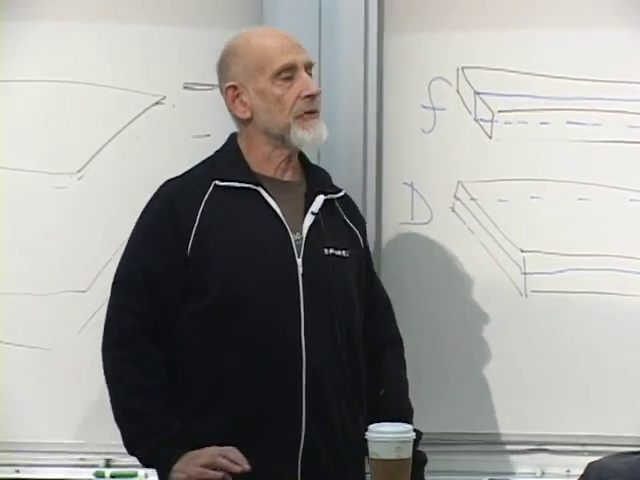
\includegraphics[width=0.78\textwidth]{lecture_01_figure_03.png}
\lectureframe{01:10:25.000}
\caption{两个缠绕膜的完整黑板状态。短与长的紧致循环产生右侧画出的类F弦与类D弦的带状结构。}
\end{figure}

一张膜可以缠绕任一紧致方向，并从非紧致方向看像一根弦。若\(R_1\)与\(R_2\)是两个圆的半径，则其有效张力为
\begin{equation}
\begin{aligned}
T_{(1)}&=2\pi R_1 T_{\mathrm{M2}},\\
T_{(2)}&=2\pi R_2 T_{\mathrm{M2}},\\
\frac{T_{(1)}}{T_{(2)}}&=\frac{R_1}{R_2}.
\end{aligned}
\end{equation}
因此不相等的圆尺寸产生不相等的弦张力。将较短的缠绕认定为轻的F弦、较长的认定为重的D弦，可以示意性地写出
\begin{equation}
g_s\sim \frac{R_{\mathrm{short}}}{R_{\mathrm{long}}},
\qquad
\frac{T_{\mathrm{D1}}}{T_{\mathrm{F1}}}\sim \frac{1}{g_s}.
\end{equation}

\begin{classroomqa}
\audiencequestion{这幅图像中的耦合能否理解为两个紧致维度之比？\lecturetimestamp{01:10:13}}
\lecturerresponse{可以。弱--强参数被几何化为一个纵横比。使一个方向变短会产生小耦合；交换两个方向则交换轻弦与重弦。}
\end{classroomqa}

\editorialnote{讲座暂时将这个比值称为\(\alpha\)，沿用了此前用于QED精细结构常数的符号。我们在此写作\(g_s\)，以保持两种含义彼此区分。在完整的M理论构造中，IIB型耦合被编码在紧致二维环面的复结构中；精确的分子取决于其循环如何标记。}

缠绕膜图像可以在不带有黑板绘图透视畸变的情况下加以概括：

\begin{figure}[htbp]
\centering
\begin{tikzpicture}[scale=1.0]
\draw[line width=0.9pt] (0,0) rectangle (5.2,2.2);
\node[below] at (2.6,-0.2) {\(R_1\)};
\node[right] at (5.4,1.1) {\(R_2\)};

\draw[->,line width=0.7pt] (5.45,1.9) -- (5.45,0.3);
\draw[->,line width=0.7pt] (5.7,0.3) -- (5.7,1.9);
\draw[->,line width=0.7pt] (0.4,-0.35) -- (4.8,-0.35);
\draw[->,line width=0.7pt] (4.8,-0.6) -- (0.4,-0.6);

\draw[line width=1.0pt] (1.1,0) -- (1.6,0) -- (1.6,2.2) -- (1.1,2.2) -- cycle;
\node at (1.35,2.55) {light};

\draw[line width=1.0pt] (0,1.45) -- (5.2,1.45);
\draw[line width=1.0pt] (0,1.00) -- (5.2,1.00);
\node at (4.55,1.95) {heavy};

\node at (1.35,-0.95) {F-string};
\node at (4.55,0.55) {D-string};
\end{tikzpicture}
\caption{两种缠绕膜构型从非紧致方向看都像弦，但不相等的紧致尺度使一根有效弦比另一根更轻。}
\end{figure}

这是早先对偶故事的几何版本。挤压一个方向同时拉伸另一个方向，会使一个缠绕对象更重而另一个更轻，因此F弦与D弦的角色可以互换。

\begin{classroomqa}
\audiencequestion{如果紧致方向是循环的，那么缠绕对象是否无限宽？\lecturetimestamp{01:10:41}}
\lecturerresponse{不是。紧致圆具有有限周长，即使可以反复绕行而不会到达边缘。剖开绘图的顶部与底部代表同一个点，正如区间的端点可以代表一个圆上的同一点。}
\end{classroomqa}

\begin{figure}[htbp]
\centering
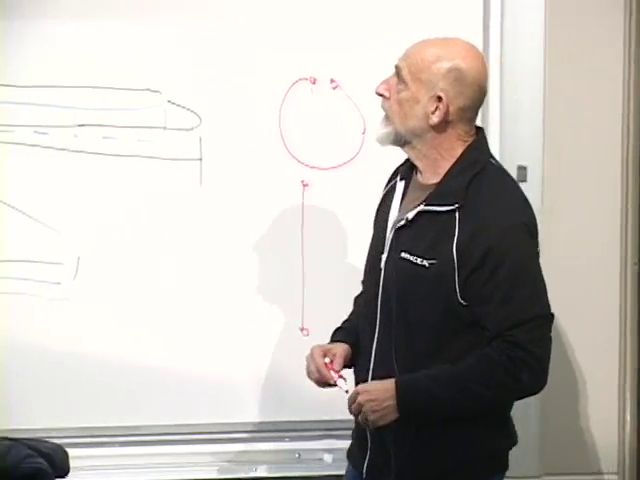
\includegraphics[width=0.78\textwidth]{lecture_01_figure_04.png}
\lectureframe{01:12:25.000}

\vspace{1em}

\begin{tikzpicture}[scale=0.95]
\draw[line width=0.9pt,->] (-3.7,0) arc[start angle=180,end angle=535,radius=0.95];
\node at (-2.75,0) {compact circle};
\draw[line width=0.9pt] (0.0,0) -- (4.8,0);
\fill (0.0,0) circle (0.06);
\fill (4.8,0) circle (0.06);
\draw[<->] (0.0,-0.45) -- (4.8,-0.45);
\node at (2.4,-0.75) {cut-open interval of length \(2\pi R\)};
\node[above] at (0.0,0.1) {same point};
\node[above] at (4.8,0.1) {same point};
\end{tikzpicture}
\caption{紧致圆及其剖开后的黑板表示。穿过一个端点会从另一个端点返回；若沿圆运动的同时也沿非紧致方向运动，则会描出一条螺旋线。}
\end{figure}

\begin{classroomqa}
\audiencequestion{为什么紧致路径是圆而不是螺旋线？\lecturetimestamp{01:12:23}}
\lecturerresponse{在非紧致方向的每个固定点处，紧致方向都是一个圆。只有当沿非紧致方向前进的同时又绕圆缠绕时，才会出现螺旋线。黑板上的区间只是把一个圆剖开，其两个端点被等同。}
\end{classroomqa}

\begin{classroomqa}
\audiencequestion{这种几何本身能否解释D膜在被近距离探测时如何看起来像一组F弦？\lecturetimestamp{01:12:49}}
\lecturerresponse{联系是存在的，但在这个初等图像中并不显然；要看出它需要更多几何工具。该图意在组织对偶，而不是推导每一个微观组成描述。}
\end{classroomqa}

\begin{classroomqa}
\audiencequestion{当在空间中移动或随时间演化时，长与短的紧致方向能否交换？\lecturetimestamp{01:13:35}}
\lecturerresponse{在理想化模型中两者皆可。压扁一个循环同时膨胀另一个循环，会交换哪根缠绕弦是轻的。这是``基本弦''只是一个名称的另一个原因：偏好的描述可以随区域或随时间而改变。}
\end{classroomqa}

\section{理想化、特殊对称点与景观}

讲座的最后一部分从优雅的对偶性例子退后一步，追问它们对真实世界说明了什么、又没有说明什么。

首先，Susskind 警告说，那些被精确控制的对偶性，是高度理想化的超对称理论的特征；在这些理论中，玻色子和费米子以完全匹配的质量出现。他将其类比为牛顿力学中的圆轨道：人们首先研究它们，是因为它们对称且数学上易于处理，而不是因为实际的行星运动可以被完美的圆穷尽。完全同样地，超对称弦理论之所以更容易分析，是因为它们比自然所显现的更为对称。

尽管如此，这种理想化仍具有启发性。一个完美的圆轨道并不是一个现实的行星系统，但它展示了在对称性较低的轨道中仍然存留的特征。同样地，超对称例子展示了量子力学、引力和微观结构能够相互协调的若干自洽方式。Susskind 刻意给出的尖锐表述是：那些易于处理的弦理论，字面上并不是关于我们世界的理论；它们的价值在于揭示了很可能在对称性较低、也更难以处理的情形中重新出现的现象。

\subsection{一个可产生许多结果的构造套件}

D-膜只是可用构造套件的一部分。讲座还提到了通量、轨形和定向轨形。人们首先选择一个紧致几何，然后选择哪些膜和通量占据它的循环。即便是简单的三明治结构，当插入一个漂浮的 D2-膜、两个或三个时，其低维物理也会发生变化。增加或减少这类成分会改变有效粒子、相互作用和参数。

假设，按照讲座的示意性计数，一个六维紧致空间大约有 \(500\) 个循环，而每个循环允许大约 \(10\) 种包裹膜、通量或相关结构的选择。那么构造的数目就像下式那样增长：
\begin{equation}
N_{\mathrm{vacua}} \sim 10^{500}.
\end{equation}
讲座的计数逻辑是初等的：
\begin{equation}
10 \times 10 \times \cdots \times 10 = 10^{500}
\end{equation}
其中有 \(500\) 个因子。DNA 类比以更熟悉的语域表达了同一点：
\begin{equation}
N_{\mathrm{DNA}}(500)=4^{500}.
\end{equation}
在 DNA 比较过程中，一位听众确认一条链上有四种选择：A、C、G 和 T。这一更正强化而非改变了论证。一份简短的局部选择清单，重复许多次，就会产生数量庞大的整体排列。确切的指数并不是重点，Susskind 称 \(10^{500}\) 是一个过时的低估；重点在于组合式的增殖。

这给出了对开头还原论期望的最终反转。复杂的粒子物理未必来自复杂的微观规则。它可能之所以出现，是因为我们的真空是许多简单成分的一种复杂排列，正如一个复杂的生物体可以由四种碱基构成的序列编码。

\begin{classroomqa}
\audiencequestion{在把由对偶性联系起来的等价描述等同之后，完整信息是否会只选出这些可能真空中的一个或少数几个，作为对我们世界的描述？\lecturetimestamp{01:26:11}}
\lecturerresponse{想必它会选出一个受限的集合，但许多不同的真空在可及能量下可能看起来极其相似。所引用的景观数目，其本意是在对偶描述被等同之后仍然很大，而不相关的高能细节可能起到像 ``垃圾 DNA 那样的作用。''}
\end{classroomqa}

\subsection{对称点与一般复杂性}

在景观之内存在特别对称的点。在几何图像中，一个等宽高比构型
\begin{equation}
R_1=R_2,
\end{equation}
使两种包裹描述同样简单。在电--磁类比中，这被示意性地表示为
\begin{equation}
m_{\mathrm{monopole}}=m_e.
\end{equation}

\begin{figure}[htbp]
\centering
\begin{tikzpicture}[scale=0.95]
\draw[line width=0.9pt] (-4.5,-1.0) rectangle (-2.5,1.0);
\draw[<->] (-4.5,-1.35) -- (-2.5,-1.35);
\draw[<->] (-2.15,-1.0) -- (-2.15,1.0);
\node at (-3.5,1.45) {symmetric point};
\node at (-3.5,-1.75) {$R_1=R_2$};

\draw[line width=0.9pt] (0.0,-0.55) rectangle (4.8,0.55);
\draw[<->] (0.0,-0.9) -- (4.8,-0.9);
\draw[<->] (5.15,-0.55) -- (5.15,0.55);
\node at (2.4,1.45) {lopsided point};
\node at (2.4,-1.3) {$R_1\ne R_2$};
\end{tikzpicture}
\caption{等宽高比的紧致化对称地对待两种包裹弦；而偏斜的紧致化使一种描述比另一种轻得多。}
\end{figure}

\begin{classroomqa}
\audiencequestion{景观中是否存在这样的真空：由于 F-弦和 D-弦描述重合，构造变得简单得多？\lecturetimestamp{01:27:21}}
\lecturerresponse{是的，存在特别对称的点。我们的世界似乎并不位于其中之一：熟悉的电粒子和磁单极子并不具有相等的质量。自然为何占据一个偏斜的点，尚不清楚。}
\end{classroomqa}

\editorialnote{电子--单极子质量相等，是一个受到适当保护的自对偶模型的示意性特征，而不是普通非超对称 QED 的预言。它表达的是讲座的对称点思想，而不是关于观测到的电子的断言。}

萨斯坎德随后回顾了通信理论中的一个类比。随机码可以极其出色，而最容易描述和解码的码则带有额外的数学结构，历史上表现反而不那么好。编码理论后来找到了极为有效的结构化构造，但这个类比依然成立：任何能被简洁命名或描述的东西，都占据着全部可能性空间中一个非常特殊、低复杂度的角落。同样，最容易计算的弦真空可能也是非典型的简单情形。

因此，恰当的问题可能会发生变化。与其要求给出每一个微观细节上的精确紧化，人们可以转而追问哪些特征在广泛的系综中是共同的或普遍的。萨斯坎德将此作为一个研究问题提出，而非已定的结论，并且拒绝以意识形态论证取代计算。

\subsection{宇宙学问题}

\begin{classroomqa}
\audiencequestion{一个周长极大的紧致方向与一个无限方向在观测上有区别吗？我们是否知道我们的三个大空间维度是无限的？\lecturetimestamp{01:30:03}}
\lecturerresponse{我们并不知道它们是无限的。一个闭合的三维球面可以在保持紧致的同时膨胀。对近平坦性的测量只给出曲率半径的下界，正如测量一片近乎平坦的田地可以限定地球的大小，却不能证明其表面是无限的。只有探测到曲率或整体认同，才能确定有限的尺度。}
\end{classroomqa}

\begin{classroomqa}
\audiencequestion{如果在理想化模型中耦合可以随空间变化，那么这种变化在现实世界中如何发生？\lecturetimestamp{01:32:43}}
\lecturerresponse{并不是像对称性示例中所用的那种不受限制的光滑变化。稍后将讨论的现实可能性，是通过具有不同有效定律的区域之间的离散跃迁来实现变化。这种跃迁是否发生是一个宇宙学问题。}
\end{classroomqa}

\editorialnote{这一回应应被理解为讲座对通量真空和畴跃迁的预告，而不是禁止一切光滑变化的标量场的一般定理。观测强烈限制无量纲耦合的变化，而稳定化机制则决定在给定模型中是否仍有连续的模可用。}

录音没有保留最后一位听众的提问。留存下来的回应说，所提出的现象对某些类型的黑洞可以发生，但不会发生在普通施瓦西黑洞的视界处，因为对自由下落的观测者而言，该视界局部上是一个普通的地方。由于问题无法可靠地复原，不再将更具体的论断归于这次交流。

\section{从砖块到描述之网}

认为物理学的更深层次必定更简单的希望已被证明是脆弱的。在\(1+1\)维玻色化中，同一理论既可以围绕费米子组织，也可以围绕玻色子组织，而费米子则作为扭结重新出现。在量子电动力学中，弱耦合与强耦合交换了电子与磁单极子的描述角色。在弦理论中，F弦与D弦重复了同样的模式，而在偶膜理论中，强耦合走得更远：一个紧致方向膨胀，D0膜变成Kaluza--Klein动量态，有效弦被重新解释为更高维几何中包裹的膜。因此，现代量子场论和弦理论并没有为``哪些是砖块，哪些是房屋？''这一问题提供唯一的、一劳永逸的答案。它们提供的是一张描述之网，每一种描述在各自的适用范围内都是高效的，同时还伴随着一个巨大的可能构造的景观，其普遍产物是复杂性而非简单性。

\chapter{几何、信息与黑洞面积定律}

\lectureoverview{所宣布的目的地是宇宙学，但通往它的最短道路始于回到狭义相对论。度规告诉我们时空的几何，而固有时为零的条件告诉我们光如何运动。我们将把这一条规则带入施瓦西几何，把视界与奇点区分开来，然后追问当黑洞辐射殆尽时信息会变成什么。答案始于普通的熵，终于贝肯斯坦的一比特论证：黑洞以视界面积而非体积为单位存储信息。}

苏斯金德暂时推迟了所承诺的对弦理论成败的清算。他说，时间已晚，实质内容比审计更有用。今晚的实质内容，是表述黑洞信息问题所需的最低限度的几何与热力学。

\section{关于光的一条规则}

狭义相对论把空间和时间当作一个几何对象。对于由\(dt,dx,dy,dz\)分隔的相邻事件，苏斯金德采用mostly-minus约定并写出
\begin{equation}
d\tau^2=dt^2-\frac{1}{c^2}\left(dx^2+dy^2+dz^2\right).
\end{equation}
时间部分与空间部分符号相反，这使闵可夫斯基几何区别于四维欧几里得几何。因子\(1/c^2\)只是协调单位；通过以相容的方式测量时间和距离，我们可以令\(c=1\)。

对于类时间隔\(d\tau^2>0\)，而\(d\tau\)是沿轨迹运动的时钟所记录的固有时。类空间隔则满足\(d\tau^2<0\)。今晚所需的情形恰好介于两者之间。光线沿\emph{零}轨迹运动，
\begin{equation}
d\tau^2=0.
\end{equation}
先限制为沿\(x\)轴的运动，得到
\begin{align}
0&=dt^2-\frac{dx^2}{c^2},\\
c\,dt&=\pm dx,\\
\frac{dx}{dt}&=\pm c.
\end{align}
这些符号描述向右和向左运动的光线。赋予\(c\)的数值在厘米被米或千米取代时会改变；不变的说法不是一个数，而是零条件。

广义相对论使度规复杂化，而不是使这条规则复杂化。以坐标\(x^\mu\)、\(\mu=0,1,2,3\)表示，
\begin{equation}
ds^2=g_{\mu\nu}(x)\,dx^\mu dx^\nu,
\end{equation}
其中重复指标求和，系数可以逐点变化。要找出局部允许的光的方向，令这个二次型为零。

\section{球坐标与施瓦西度规}

不旋转的黑洞是球对称的，因此笛卡尔坐标掩盖了有用的结构。令\(r\)度量径向距离，令\(\theta,\phi\)确定单位球面上的方向。其线元为
\begin{equation}
d\Omega^2=d\theta^2+\sin^2\theta\,d\phi^2.
\end{equation}
因此在半径为\(r\)的球面上，角位移贡献\(r^2d\Omega^2\)。球坐标下的平直时空为
\begin{equation}
d\tau^2=dt^2-\left(dr^2+r^2d\Omega^2\right),
\qquad (c=1).
\end{equation}

苏斯金德没有从爱因斯坦方程推导黑洞解。他把它写下来，并要求我们审视它。黑板明确地作出了预期的比较。

\begin{figure}[htbp]
\centering
\includegraphics[width=0.86\textwidth]{lecture_02_figure_02.png}
\caption{施瓦西形变之上的平直球面时空。重复出现的因子\(1-2GM/(c^2r)=1-R_s/r\)与径向草图同时可见。}
\lectureframe{00:19:12.520}
\end{figure}

对于质量为\(M\)的黑洞，定义施瓦西半径
\begin{equation}
R_s=\frac{2GM}{c^2}.
\end{equation}
外部线元为
\begin{equation}
d\tau^2=\left(1-\frac{R_s}{r}\right)dt^2
-\frac{dr^2/c^2}{1-R_s/r}
-\frac{r^2}{c^2}d\Omega^2.
\label{eq:schwarzschild-explicit-c}
\end{equation}
等价地，在令\(c=1\)之后，
\begin{equation}
ds^2=\left(1-\frac{2GM}{r}\right)dt^2
-\frac{dr^2}{1-2GM/r}-r^2d\Omega^2.
\label{eq:schwarzschild}
\end{equation}
在远处，\(R_s/r\ll1\)，平直球面度规回归。这个渐近检验比记住公式更重要，尽管苏斯金德推荐后者作为鸡尾酒会上的谈资。

\editorialnote{黑板在\(d\tau^2\)与\(ds^2\)之间交替，并且没有一致地显示每一个\(c\)因子。方程~\eqref{eq:schwarzschild-explicit-c}遵循讲座的时间坐标约定，其中\(t\)具有时间的量纲。带有\(x^0=ct\)的标准形式在代数上等价。}

\subsection{视界不是奇点}

在坐标中有两个半径看起来可疑。在自然单位下的\(r=R_s=2GM\)处，\(dt^2\)的系数为零，而\(dr^2\)的系数发散。在\(r=0\)处，曲率本身变为奇异。这些不是同一事件的两种版本：
\begin{equation}
\begin{aligned}
r=R_s &:\quad \text{horizon},\\
r=0 &:\quad \text{curvature singularity}.
\end{aligned}
\end{equation}

潮汐力给出了物理上的区分。引力场在延展物体上逐点变化：脚受到的拉力可能比头更强，拉伸身体，而横向方向被挤压。在视界处，这些潮汐力是有限的，而在质量足够大的黑洞的视界处，它们可以非常小。那里不必发生任何局部灾难性的事情。相反，在\(r=0\)处，潮汐力发散。\(r=R_s\)处令人警觉的系数标志着施瓦西坐标的缺陷；\(r=0\)处的奇点是物理的。

\editorialnote{曲率在\(r=R_s\)处的有限性可由Kretschmann标量\(R_{\mu\nu\rho\sigma}R^{\mu\nu\rho\sigma}=48G^2M^2/(c^4r^6)\)来检验，该标量在视界处有限，仅在\(r\to0\)时发散。这一不变量在讲座中并未写出，但它使潮汐力的区分变得精确。}

\section{视界附近的径向光}

现在回到那条规则。径向光线保持其角位置固定，因此\(d\Omega=0\)，而光线满足\(ds^2=0\)。在\(c=1\)单位下，方程~\eqref{eq:schwarzschild}给出
\begin{equation}
0=\left(1-\frac{2GM}{r}\right)dt^2
-\frac{dr^2}{1-2GM/r}.
\end{equation}
乘以\(1-2GM/r\)并取平方根得到两个分支，
\begin{align}
dr&=\pm\left(1-\frac{2GM}{r}\right)dt,\\
\frac{dr}{dt}&=\pm\left(1-\frac{2GM}{r}\right).
\label{eq:radial-null}
\end{align}
正号对应出射，负号对应入射。在远处，它们的坐标速度趋近于\(\pm1\)。在视界处，两者都满足\(\lvert dr/dt\rvert\to0\)：在Schwarzschild坐标时间中，出射光线似乎在那里静止不动，而入射光线则需要无限长的坐标时间才能到达。

\begin{figure}[htbp]
\centering
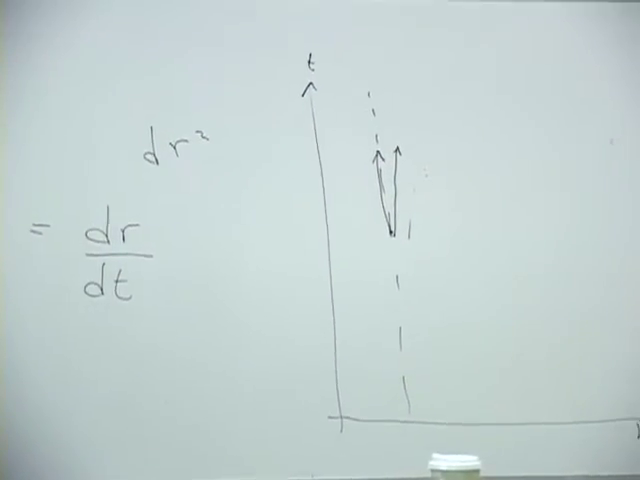
\includegraphics[width=0.82\textwidth]{lecture_02_figure_03.png}
\caption{完成的\(t\)-\(r\)黑板草图：当接近虚线视界时，径向零测地线变得几乎竖直。}
\lectureframe{00:30:25.000}
\end{figure}

\begin{figure}[htbp]
\centering
\begin{tikzpicture}[x=1.0cm,y=0.9cm]
\draw[->] (0,0) -- (6.6,0) node[right] {$r$};
\draw[->] (0,0) -- (0,6.2) node[above] {$t$};
\draw[dashed,thick] (2.0,0) -- (2.0,5.9) node[above] {$r=R_s$};
\draw[thick,->] (2.08,.4) .. controls (2.10,2.2) and (2.55,3.8) .. (5.8,5.7);
\draw[thick,->] (5.8,.5) .. controls (3.2,2.0) and (2.15,4.2) .. (2.03,5.7);
\node[align=center] at (4.7,4.4) {outgoing};
\node[align=center] at (4.5,1.2) {ingoing};
\end{tikzpicture}
\caption{黑板草图的坐标时间清理版本。表观减慢是关于Schwarzschild \(t\)的陈述，而不是关于光在局部未能以\(c\)运动的陈述。}
\end{figure}

在视界内部，未来光锥向内倾斜得如此厉害，以至于两个指向未来的径向分支都通向\(r\)减小的方向。任何源自那里的信号都无法逃逸到外部，而每一条指向未来的因果路径都到达奇点。

\begin{classroomqa}
\audiencequestion{如果光速是不变的，那么说光在视界附近减慢究竟是什么意思？\lecturetimestamp{00:31:44}}
\lecturerresponse{所展示的量是在特定坐标系中的\(dr/dt\)。当米被厘米取代时，数值速度就已经改变；在这里，有效的径向和时间标定随位置而变化。普遍的陈述是，每一条光线都遵循零测地线轨迹，\(ds^2=0\)。}
\end{classroomqa}
\editorialnote{自由下落的局部观测者测得真空中的光速为\(c\)；视界处Schwarzschild坐标速度的消失并不是局部可观测量。}

\begin{classroomqa}
\audiencequestion{无论光通过何种物质介质传播，同样的零速度陈述都成立吗？\lecturetimestamp{00:33:24}}
\lecturerresponse{不。现有的认识不再保留对此答案的解释。}
\end{classroomqa}
\editorialnote{零速度论断涉及真空时空中的传播。与物质的相互作用可以使波包具有较小的有效速度；那是介质的性质，而不是局部因果速度\(c\)的改变。}

\begin{classroomqa}
\audiencequestion{在同一個\(t\)-\(r\)图上，入射光线看起来是什么样子？\lecturetimestamp{00:33:32}}
\lecturerresponse{它是看起来反向的分支：从大的\(r\)出发，它向视界弯曲并渐近地接近它。它需要无限多的坐标时间\(t\)才能到达。}
\end{classroomqa}
\editorialnote{下落的观测者在有限的固有时内到达并穿过视界；只有Schwarzschild \(t\)发散。}

\section{为什么蒸发会产生问题}

视界值得更多的研究：它如何形成，下落的观测者看到什么，以及那里是否发生任何局部异常的事情。Susskind推迟了这些问题，直接跳到量子力学。从外部看，物质及其所有可区分的信息被挤压得越来越靠近视界，变得不可获取。仅此一点未必会摧毁信息；它可能只是将其隐藏起来。

Hawking的结果使问题变得尖锐。一个稳定的经典黑洞看起来像可以想象的最乏味的物体：球形、黑暗、无法发送信息。但``黑''有两种含义。它可以意味着不发射任何东西，也可以意味着发射热黑体辐射。量子黑洞是在第二种意义上黑的。它有温度，会发光，并损失能量。由于
\begin{equation}
E=Mc^2,
\qquad
R_s=\frac{2GM}{c^2},
\end{equation}
辐射会同时减小其质量和视界半径。如果蒸发最终移除了黑洞，那么似乎留在其视界处的信息会变成什么？它可能被摧毁，被困在微小的遗迹中，或被编码在出射辐射中。这些可能性之间的张力就是信息问题，而弦理论后来将有助于使它的解决变得更加清晰。

今晚不尝试对弯曲时空中的量子场进行计算。相反，Susskind遵循Bekenstein更简单的路线：首先将熵理解为信息，然后计算黑洞能隐藏多少信息。

\section{存在但被隐藏的信息}

设想把一个盒子划分成足够小的格子，使得每个格子要么被占据，要么为空。每个格子对应一个答案的二进制串---one answer per cell---把该位形与所有其他允许的位形区分开来。更现实的物质需要对粒子种类和其他自由度提出问题，但原理不变：信息由指定状态所需的最少是--否问题数来衡量。

\begin{classroomqa}
\audiencequestion{这只是对一个静态系统的描述吗？\lecturetimestamp{00:45:49}}
\lecturerresponse{这是瞬时的描述，即在一个时刻。动力学随后把该状态映射到另一个状态。}
\end{classroomqa}

下一个原理更为深刻：闭合系统的演化不会把两个不同的微观状态合并为一个。如果两个位形现在不同，它们演化后的位形在原则上仍可区分。经典哈密顿演化是可逆的，量子演化是幺正的。\editorialnote{耗散型有效方程之所以能抹去区别，只是因为未被观测的环境自由度被省略了；完整的闭合状态仍保留它们。}

浴缸把损失与不可及之间的区别具体化。两股水滴流可以编码两段不同的摩尔斯电码文本。水静下来之后，两个浴缸看起来一样。可见的涟漪已经消失，但完整的微观测量仍会发现不同的分子位形。信息已经扩散到太小、太多而无法追踪的自由度中。

熵就是这种隐藏的信息。相对于我们能提出的宏观问题---温度、总能量、成分、水位---许多微观区别仍然可能但不可及。用讲座中数比特的语言，
\begin{equation}
S=\hbox{number of hidden bits}.
\end{equation}
精确的统计公式是\(S=k_B\ln\Omega\)，但定性的定义对黑洞论证已经足够。

\section{温度作为隐藏一个比特的代价}

温度测量起来很熟悉，定义起来却出人意料地间接。Susskind选择熵和能量作为原始概念。假设一个计算机比特被重置到标准值。物理装置仍然存在，但它先前零态和一态之间的区别从计算机中消失了。它不可能从完整世界中消失；它被转移到环境中的微观自由度，使环境轻微升温。这就是Landauer原理。

如果一个熵单位是一个比特，温度以能量单位度量，讲座写出
\begin{align}
\Delta S&=1,\\
\Delta E&=T\,\Delta S,\\
dE&=T\,dS.
\label{eq:first-law}
\end{align}

\begin{figure}[htbp]
\centering
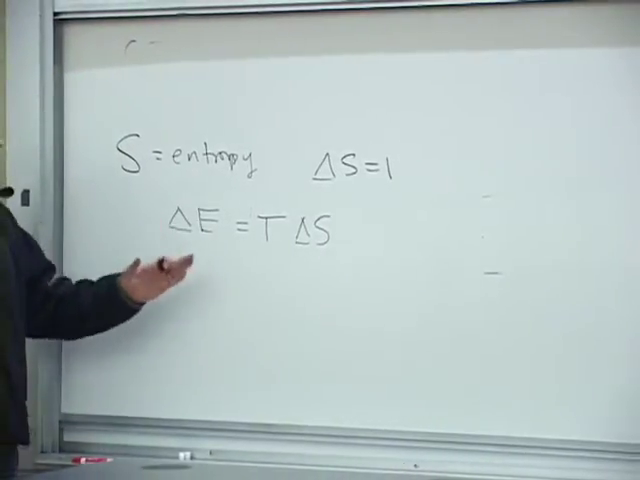
\includegraphics[width=0.84\textwidth]{lecture_02_figure_04.png}
\caption{黑板上的信息论热力学：\(S\)是熵，一个隐藏比特有\(\Delta S=1\)，其最小能量代价写作\(\Delta E=T\Delta S\)。}
\lectureframe{00:58:40.000}
\end{figure}

\editorialnote{在常规单位下，一个二进制比特的可逆擦除代价是\(k_BT\ln2\)。方程~\eqref{eq:first-law}使用\(k_B=1\)，并把讲座的熵单位视为一个比特，同时略去相关的\(\ln2\)。这些约定不影响随后的标度论证。}

听众的估计给出：把大约\(100\)吉字节擦除到一杯水中，引起的最低温升接近\(10^{-15}\)度。Susskind接受这一要点而非确切数字：在室温下，一个比特携带极小的最小能量，而真实计算机耗散得多得多，因为擦除并非可逆地进行。

\begin{classroomqa}
\audiencequestion{硬盘的例子只是类比，还是擦除致热是一条真实的定律？\lecturetimestamp{01:00:02}}
\lecturerresponse{它是一条真实的物理约束，即Landauer规则。重置一个存储单元把旧的区别从计算机中移除，因此该信息必须被带入环境。普通操作的效率远低于理想最小值，因为它们还驱动电路、移动电荷并产生无关的热。}
\end{classroomqa}

\begin{classroomqa}
\audiencequestion{在更高温度下隐藏一个比特要花费更多能量吗？\lecturetimestamp{01:02:07}}
\lecturerresponse{是的。关系\(dE=T\,dS\)正是这样说的：对于相同的熵转移，更热的热浴需要更大的能量转移。人们同样可以把这种每隐藏比特的能量关系视为温度的定义。}
\end{classroomqa}

\begin{classroomqa}
\audiencequestion{如果覆盖一个先前存储的比特，那个旧信息已经丢失了吗？\lecturetimestamp{01:02:43}}
\lecturerresponse{它已经离开计算机，但并未从闭合物理系统中消失。被覆盖的区别已经散布到环境中，在那里它贡献不可及的信息，因而贡献熵。}
\end{classroomqa}

将热力学熵等同于缺失的微观信息，这一思想可追溯到玻尔兹曼；香农在二十世纪给出了与之对应的信息论语言。苏斯金德指出，在他和听众中的一些人在1950年代所接触的热力学课程中，这种解释奇怪地缺席了。计算机科学使这一联系更难被忽视，但并未创造其物理内容。

\section{将一比特放入黑洞}

现在我们可以概念性地逐比特构建一个黑洞，就像浴缸可以逐滴注满一样。问题在于微分层面：当额外一比特被隐藏时，视界增长了多少？从质量为\(M\)、半径为\(R_s\)的黑洞出发，然后送入最简单的物体，其唯一可恢复的区别仅在于是否被吸收。

\begin{classroomqa}
\audiencequestion{信息进入黑洞难道不需要无限坐标时间吗？\lecturetimestamp{01:08:07}}
\lecturerresponse{它在视界附近被指数压缩，在很短的实用时间内对外部不可用，尽管施瓦茨席尔德坐标时间将实际穿越赋予无限值。因此对于外部记账而言，它可以被视为存储在视界上。}
\end{classroomqa}

光子是一个自然的候选者，但一般的光子携带的信息不止一比特。其偏振可以编码一个二元选择。一个高度局域化的到达点提供了许多进一步的是--否问题：上半球还是下半球，左半还是右半，等等。量子力学将局域化限制在约一个波长，因此抑制位置信息的方法是使用黑洞仍能吸收的最长波长。

\begin{classroomqa}
\audiencequestion{真的存在一个光子无法进入的上限波长吗？\lecturetimestamp{01:12:15}}
\lecturerresponse{是的。远大于黑洞的波主要被散射而非吸收。有用的临界选择是波长与视界半径相当：足够长以抹去进入点，又足够短以具有可观的吸收概率。}
\end{classroomqa}

\begin{classroomqa}
\audiencequestion{光子到达的方向本身是否增加了信息？\lecturetimestamp{01:13:28}}
\lecturerresponse{对于与整个视界同量级的波长，场在黑洞上的变化如此缓慢，以至于到达方向无法以精细精度分辨。这就是为什么长波长极限近似为单个是--否数据，而非一个锐利定位的撞击。}
\end{classroomqa}

因此，在量级上选择
\begin{equation}
\lambda\sim R_s=\frac{2GM}{c^2}.
\label{eq:one-bit-wave}
\end{equation}
光子运动学给出
\begin{equation}
E=cp,
\qquad
p=\hbar k=\frac{h}{\lambda},
\qquad
\Delta E\sim\frac{\hbar c}{R_s}.
\label{eq:one-bit-energy}
\end{equation}
这里\(k=2\pi/\lambda\)和\(h=2\pi\hbar\)。讲座刻意忽略了\(2\pi\)，以及量级为一的吸收因子。

\begin{classroomqa}
\audiencequestion{动量应该写成\(\hbar/\lambda\)，还是\(h/\lambda\)？\lecturetimestamp{01:16:00}}
\lecturerresponse{以\(\lambda\)为普通波长时，精确关系是\(p=h/\lambda=2\pi\hbar/\lambda\)；以波数\(k=2\pi/\lambda\)表示时，则是\(p=\hbar k\)。当前的估计只保留量级，因此因子\(2\pi\)被有意舍弃。}
\end{classroomqa}

隐藏一比特的能量代价是温度标度。方程~\eqref{eq:one-bit-wave}和~\eqref{eq:one-bit-energy}因此给出
\begin{equation}
k_BT_H\sim\frac{\hbar c}{R_s}
\sim\frac{\hbar c^3}{GM}.
\end{equation}
精确的霍金结果是
\begin{equation}
k_BT_H=\frac{\hbar c^3}{8\pi GM}.
\end{equation}
基本论证得到了对\(M,G,c,\hbar\)的依赖关系，但未得到系数。

\section{一比特占据一个普朗克尺度斑块}

同一个光子告诉我们视界如何增长。其能量使质量改变
\begin{equation}
\Delta M=\frac{\Delta E}{c^2}
\sim\frac{\hbar}{cR_s}.
\end{equation}
由于\(R_s=2GM/c^2\)，
\begin{equation}
\Delta R_s=\frac{2G}{c^2}\Delta M
\sim\frac{G\hbar}{c^3R_s},
\end{equation}
其中所有量级为一的因子再次被抑制。乘以\(R_s\)，
\begin{equation}
R_s\Delta R_s\sim\frac{G\hbar}{c^3}.
\end{equation}
因为\(A=4\pi R_s^2\)，其微分为\(dA=8\pi R_s\,dR_s\)。因此
\begin{equation}
\Delta A\sim\frac{G\hbar}{c^3}=\ell_P^2,
\qquad
\ell_P=\sqrt{\frac{G\hbar}{c^3}}.
\label{eq:planck-patch}
\end{equation}

\begin{figure}[htbp]
\centering
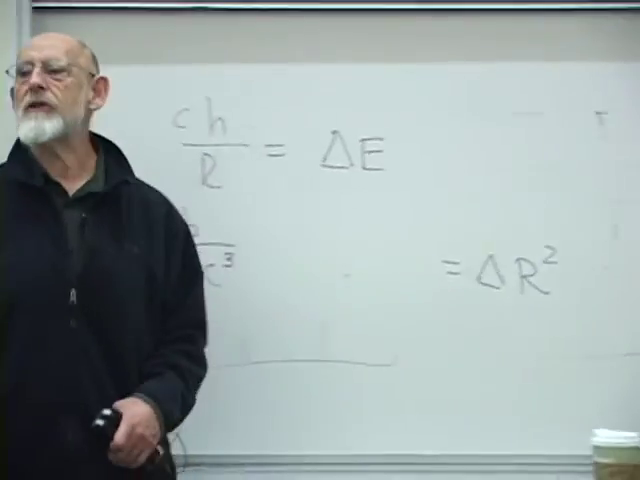
\includegraphics[width=0.84\textwidth]{lecture_02_figure_05.png}
\caption{黑板上完成的标度论证：一比特能量\(\Delta E\sim\hbar c/R_s\)导致半径平方、因而面积的增量约为\(G\hbar/c^3\)。}
\lectureframe{01:22:40.000}
\end{figure}

在现场计算过程中，\(c\)的因子在中途被恢复，一位听众发现了施瓦茨席尔德半径中缺失的\(c^{-2}\)。正是这一修正产生了方程~\eqref{eq:planck-patch}中的\(c^{-3}\)。

\begin{classroomqa}
\audiencequestion{仅在计算的一部分中恢复\(c\)，是否丢失了它的两个幂次？\lecturetimestamp{01:21:18}}
\lecturerresponse{是的。量纲关系是\(R_s=2GM/c^2\)，而非简单的\(2GM\)。恢复该因子使面积标度为\(G\hbar/c^3\)。}
\end{classroomqa}

利用\(G\simeq6.7\times10^{-11}\,\mathrm{m^3\,kg^{-1}\,s^{-2}}\)、\(\hbar\simeq1.05\times10^{-34}\,\mathrm{J\,s}\)和\(c^3\simeq2.7\times10^{25}\,\mathrm{m^3\,s^{-3}}\)，
\begin{equation}
\ell_P^2\simeq2.6\times10^{-70}\,\mathrm{m^2},
\qquad
\ell_P\simeq1.6\times10^{-35}\,\mathrm{m}.
\end{equation}
讲座中口头说出的幂次在黑板上进行估计时有所游移；物理结论是稳定的。这一尺度远低于直接实验分辨率。

令人难忘的图景是：不可穿透的比特带着尖锐的棱角，在视界上堆积，并彼此挤开。每个新比特大约占据一个普朗克面积的斑块。这是对面积记账的一种比喻，并不是说字面意义上的方形瓷砖构成了视界。

\begin{classroomqa}
\audiencequestion{如果第一个光子仍在接近时，另一个光子扩大了视界，那么旧光子难道不会落入新视界之内吗？\lecturetimestamp{01:26:39}}
\lecturerresponse{简单的静态图景不够精确，无法解决这个问题。动态时空中的事件视界必须全局地定义，其位置随着物质到达而改变。在此处所用的外部描述中，信息仍与不断增长的视界相关联。对该视界的精确定义将推迟给出。}
\end{classroomqa}

\begin{classroomqa}
\audiencequestion{当加入巨大质量时，例如两个黑洞碰撞时，会出现同样的问题吗？\lecturetimestamp{01:27:03}}
\lecturerresponse{是的；那时动态特征就无法忽视了。讲座将完整的并合几何推迟到视界被更仔细地定义之后。}
\end{classroomqa}

\begin{classroomqa}
\audiencequestion{普朗克面积是只在平坦斑块上定义的，而不是在球面视界上定义的吗？\lecturetimestamp{01:27:30}}
\lecturerresponse{它是球面上的一个面积尺度，并不要求视界是平坦的。对于这种计数而言，平面与球面的区分并不重要。}
\end{classroomqa}
\editorialnote{当视界曲率半径远大于\(\ell_P\)时，每个普朗克尺度的邻域局部上几乎都是平坦的。}

对于一个直径八公里的黑洞，边缘光子相应地是波长约为该尺度的长射电波。一个面向听众的类比将这种与尺寸无关的面积增量，比作给绕篮球或绕地球的绳子增加相同的额外周长：在每种情况下，由固定增加的周长所产生的径向间隙都相同。精确几何有所不同，但两个例子都分离出了一种与物体原有尺寸无关的变化。

\section{面积定律}

一次增加一个比特，会使视界面积改变一个普适的微观量。因此，能够被隐藏的比特数必须正比于\(A/\ell_P^2\)，而不是正比于体积。贝肯斯坦推断出了这种正比关系；霍金的计算确定了其系数：
\begin{equation}
S_{\mathrm{BH}}=\frac{k_B A c^3}{4G\hbar}
=\frac{k_B A}{4\ell_P^2}.
\label{eq:bh-entropy}
\end{equation}
如果用二进制比特而不是热力学单位来计数熵，则将\(S_{\mathrm{BH}}/k_B\)除以\(\ln2\)。

\begin{figure}[htbp]
\centering
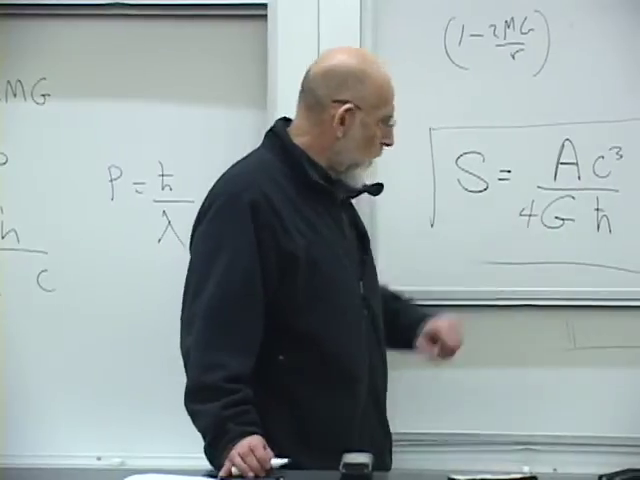
\includegraphics[width=0.84\textwidth]{lecture_02_figure_06.png}
\caption{最终写在黑板上的公式，包括霍金的因子\(1/4\)：在讲座的熵单位中为\(S\propto Ac^3/(4G\hbar)\)。}
\lectureframe{01:31:02.000}
\end{figure}

因此，黑洞比大小相当的普通系统具有更多的熵，而且多出极大的幅度。然而，这个答案仍然小于朴素体积计数可能暗示的结果。独立信息受一个表面测度所界定。这种反转---一个三维的引力区域，由按二维边界标度的信息来描述---正是全息原理的种子。

\begin{classroomqa}
\audiencequestion{熵公式中的因子\(1/4\)从何而来？\lecturetimestamp{01:30:30}}
\lecturerresponse{贝肯斯坦的论证确定了它对面积和基本常数的依赖关系，但留下了一个未知系数；他的估计产生了诸如二的 logarithm 之类的可能性。霍金的量子场计算将该系数精确确定为\(1/4\)。}
\end{classroomqa}

\(\hbar\)的位置包含了最后的惊奇。人们可能期望量子熵正比于\(\hbar\)，并在经典极限下消失。相反，\(\hbar\)出现在分母中。当\(\hbar\to0\)时，波可以以任意小的能量代价携带任意精细的信息，因此熵容量发散。量子化并没有给一个原本经典的洞加上微小的熵；它阻止了信息容量变为无限。

\begin{classroomqa}
\audiencequestion{为什么\(\hbar\)，其单位是角动量，也决定了普通动量与波长之间的关系？\lecturetimestamp{01:33:23}}
\lecturerresponse{\(\hbar\)具有作用量的单位，等价于动量乘以距离。由于\(p\lambda\)具有相同的单位，量子关系可以写成\(p\sim\hbar/\lambda\)，最多相差\(2\pi\)的约定。角动量\(\mathbf r\times\mathbf p\)出于同样的原因具有相同的量纲。}
\end{classroomqa}

讲座到此为止，并非因为主题已经穷尽，而是因为这是一个恰当的边界。几何学已经告诉我们视界为何隐藏信息；热力学已经告诉我们如何计数被隐藏的信息；量子力学则提供了每比特所对应的有限面积。下一个问题不再是黑洞是否具有微观状态，而是这些状态如何编码并最终归还落入其中的东西。

\chapter{平坦坐标中的视界与蒸发的热力学}

\lectureoverview{Schwarzschild 度规在视界处似乎变得奇异，尽管自由下落的观测者在那里不应注意到任何异常。我们通过将近视界度规转换为双曲极坐标下的平坦 Minkowski 空间来解决这一矛盾。同一几何随后将 Alice 的坠落描述与 Bob 的加速外部描述区分开来。后半部分展开熵与温度，推导 Hawking 的逆质量温度与 \(M^3\) 蒸发定律，并以追问信息守恒对引力的微观理论提出什么要求作结。}

\section{\texorpdfstring{\(r=2GM\)}{r=2GM}处的疑难}

从一个非常大的黑洞开始。其视界的曲率可以小到使一个穿过它的观测者在任何适度的实验室尺度区域内看到几乎空无一物的平坦时空。没有墙被撞上，也没有局部警报宣告穿越。然而 Schwarzschild 度规似乎说，恰好在那个半径处发生了某种奇异的事情。本讲前半部分的目的就是使这两个陈述相容。

我们采用 mostly-plus 号差约定。在平坦时空中，
\begin{equation}
ds^2=-dt^2+dx^2+dy^2+dz^2,
\end{equation}
因此类时世界线有 \(ds^2<0\)，固有时满足 \(d\tau^2=-ds^2\)。这是上一讲所用约定整体符号的反转；没有任何可观测量依赖于这一选择。

取 \(c=1\)，Schwarzschild 线元为
\begin{equation}
\begin{aligned}
ds^2={}&-\left(1-\frac{2GM}{r}\right)dt^2
+\frac{dr^2}{1-\frac{2GM}{r}}
+r^2d\Omega_2^2,\\
d\Omega_2^2={}&d\theta^2+\sin^2\theta\,d\phi^2 .
\end{aligned}
\label{eq:l03-schwarzschild}
\end{equation}
Schwarzschild 半径为 \(R_s=2GM\)，或当恢复 \(c\) 时为 \(R_s=2GM/c^2\)。在远处，\(r\gg R_s\)，两个径向系数都趋近其平坦空间值。然而在 \(r=R_s\) 处，\(dt^2\) 的系数为零，而 \(dr^2\) 的系数发散。这看起来颇具戏剧性。问题在于几何本身具有戏剧性，还是仅仅坐标如此。

\section{坐标的两条教训}

\subsection{极坐标的无害起源}

在普通欧几里得平面上，
\begin{equation}
ds^2=dx^2+dy^2.
\end{equation}
引入极坐标
\begin{equation}
x=\rho\cos\theta,
\qquad
y=\rho\sin\theta .
\end{equation}
微小位移的径向长度为 \(d\rho\)，横向长度为 \(\rho\,d\theta\)，因此
\begin{equation}
ds^2=d\rho^2+\rho^2d\theta^2.
\label{eq:l03-polar}
\end{equation}
在 \(\rho=0\) 处，角向系数为零。这并不使平面的中心奇异。它只是说，在那里 \(\theta\) 的每一个值都命名同一个点。因此，一个奇特的度规系数可能诊断的是一个奇特的坐标系，而非奇特的物理。

\subsection{双曲极坐标}

现在把欧几里得平面替换为 \(1+1\) 维 Minkowski 时空，
\begin{equation}
ds^2=-dT^2+dX^2.
\end{equation}
在右手楔形区 \(X>|T|\) 中，定义
\begin{equation}
X=\rho\cosh\omega,
\qquad
T=\rho\sinh\omega,
\qquad \rho>0 .
\label{eq:l03-rindler-transform}
\end{equation}
普通的恒等式 \(\cos^2\theta+\sin^2\theta=1\) 被替换为
\begin{equation}
\cosh^2\omega-\sinh^2\omega=1.
\end{equation}
因此，常 \(\rho\) 线是双曲线
\begin{equation}
X^2-T^2=\rho^2.
\end{equation}
与周期性的角 \(\theta\) 不同，类快度坐标 \(\omega\) 从 \(-\infty\) 延伸到 \(+\infty\)。在大的正 \(\omega\) 处，\(\cosh\omega\) 与 \(\sinh\omega\) 变得几乎相等，双曲线趋近未来零射线 \(X=T\)。

对式~\eqref{eq:l03-rindler-transform}求导给出
\begin{align}
dX&=\cosh\omega\,d\rho+\rho\sinh\omega\,d\omega,\\
dT&=\sinh\omega\,d\rho+\rho\cosh\omega\,d\omega .
\end{align}
交叉项相消，留下
\begin{equation}
ds^2=-\rho^2d\omega^2+d\rho^2.
\label{eq:l03-rindler-metric}
\end{equation}

\begin{figure}[htbp]
\centering
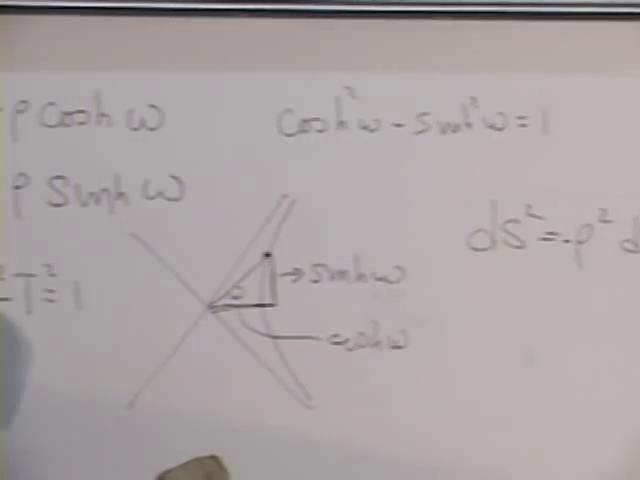
\includegraphics[width=0.72\textwidth]{lecture_03_figure_02.png}
\caption{完成后的双曲坐标板书：\(X=\rho\cosh\omega\)、\(T=\rho\sinh\omega\)、单位双曲线构造，以及形式为 \(ds^2=-\rho^2d\omega^2+d\rho^2\) 的平坦度规。}
\lectureframe{00:16:55.000}
\end{figure}

式~\eqref{eq:l03-rindler-metric}仍然描述完全平坦的时空。其时间系数在 \(\rho=0\) 处为零，正如式~\eqref{eq:l03-polar}的角向系数在原点处为零一样。坐标图在那里退化；时空并不退化。

\section{放大 Schwarzschild 视界}

回到式~\eqref{eq:l03-schwarzschild}的径向-时间部分：
\begin{align}
ds^2
&=-\frac{r-2GM}{r}\,dt^2
+\frac{r}{r-2GM}\,dr^2 .
\label{eq:l03-rewritten-schwarzschild}
\end{align}
我们现在只考察 \(r=2GM\) 的一个狭窄邻域。在变化缓慢的因子中，\(r\) 可以用 \(2GM\) 替换。因子 \(r-2GM\) 必须保留，因为它在视界处为零并改变符号。因此
\begin{equation}
ds^2\approx
-\frac{r-2GM}{2GM}\,dt^2
+\frac{2GM}{r-2GM}\,dr^2 .
\label{eq:l03-near-horizon-r}
\end{equation}

选择一个新的径向坐标 \(\rho\)，使第二项简单地成为 \(d\rho^2\)：
\begin{equation}
d\rho^2=\frac{2GM}{r-2GM}\,dr^2.
\end{equation}
在视界外，取正平方根并从 \(r=2GM\) 积分给出
\begin{align}
d\rho&=\sqrt{\frac{2GM}{r-2GM}}\,dr,\\
\rho&=2\sqrt{2GM}\sqrt{r-2GM},\\
\rho^2&=8GM(r-2GM),
\qquad
r-2GM=\frac{\rho^2}{8GM}.
\label{eq:l03-rho-r}
\end{align}
代入式~\eqref{eq:l03-near-horizon-r}得到
\begin{equation}
ds^2\approx
-\frac{\rho^2}{16G^2M^2}\,dt^2+d\rho^2.
\end{equation}
最后重新标度 Schwarzschild 时间，
\begin{equation}
\omega=\frac{t}{4GM},
\qquad
d\omega^2=\frac{dt^2}{16G^2M^2},
\label{eq:l03-omega}
\end{equation}
并得到
\begin{equation}
\boxed{ds^2\approx-\rho^2d\omega^2+d\rho^2.}
\label{eq:l03-near-horizon-rindler}
\end{equation}

\begin{figure}[htbp]
\centering
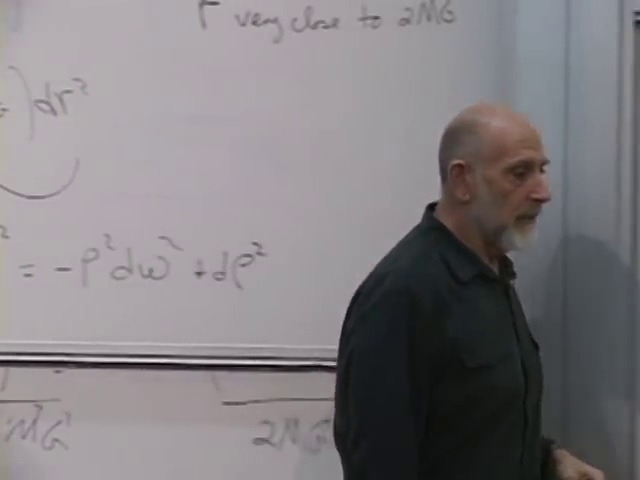
\includegraphics[width=0.70\textwidth]{lecture_03_figure_03.png}
\caption{时间重新标度后的板书：近视界 Schwarzschild 度规已变成与平坦 Minkowski 时空相同的双曲极坐标度规。}
\lectureframe{00:31:35.000}
\end{figure}

当所考察的邻域向视界收缩时，该近似会无限地改善。它证明了我们想要的局部陈述：对于一个足够大的洞，视界就是写在非凡坐标系中的普通时空。对于有限质量的施瓦西洞，曲率并非字面意义上的零，但它在视界处是有限的，并且可以通过增大\(M\)使它在视界处任意小。\editorialnote{局部曲率标度的量级为\(R_s^{-2}\)。林德勒度规是局部近视界展开中的领头项，而不是声称整个施瓦西几何全局平坦。}

\begin{classroomqa}
\audiencequestion{对于\(r<2GM\)，方程~\eqref{eq:l03-rho-r}使这个外部\(\rho\)成为虚数。这是否标志着物理问题？\lecturetimestamp{00:32:30}}
\lecturerresponse{它以不同的形式再现了同样的坐标失效。当前的坐标图是为外部楔形构造的；要延伸穿过视界需要另一个坐标图。这个特定\(\rho\)的失效并不是视界处的物理事件。}
\end{classroomqa}

\begin{classroomqa}
\audiencequestion{在近视界改写中，近似后的线如何从前面的精确线得出？\lecturetimestamp{00:39:21}}
\lecturerresponse{只有\(r\)中缓慢变化的出现被设为等于\(2GM\)。小差值\(r-2GM\)被保留不变。这就是该近似，并且当\(r\)趋近\(2GM\)时它变得越来越精确。}
\end{classroomqa}

\section{坐标的含义}

该变换确认
\begin{equation}
\rho=0\quad\Longleftrightarrow\quad r=2GM.
\end{equation}
外部\(r>2GM\)是右林德勒楔形\(X>|T|\)。恒定\(\rho\)双曲线代表保持在固定施瓦西半径处的观测者。在该楔形中任何地方发出的出射光线都会穿过每一条更大的\(\rho\)世界线，因此外部观测者可以向外通信。未来零边界之外的点无法将光信号发送回右楔形。那条零边界就是视界。

\begin{classroomqa}
\audiencequestion{这里展示的双曲坐标片是否总是描述视界之外的区域？\lecturetimestamp{00:35:22}}
\lecturerresponse{是的。在此构造中\(r>2GM\)给出\(\rho^2>0\)并将事件置于右外部楔形中。零边缘\(\rho=0\)是视界；当前坐标不会作为实外部坐标继续延伸到它之外。}
\end{classroomqa}

\begin{classroomqa}
\audiencequestion{恒定\(\rho\)双曲线代表一个时间还是一个距离？\lecturetimestamp{00:37:21}}
\lecturerresponse{在近视界近似中，它代表到视界的一个固定固有距离，因此也代表一个固定的施瓦西半径。沿双曲线的运动就是驻扎在那里的观测者的时间流逝。}
\end{classroomqa}

沿固定\(\rho\)轨迹，方程~\eqref{eq:l03-rindler-metric}给出
\begin{equation}
d\tau=\rho\,d\omega.
\label{eq:l03-proper-time-rindler}
\end{equation}
因此\(\omega\)本身并不是观测者的固有时间。它是双曲线族共有的角时间；每个观测者将它乘以该观测者的\(\rho\)，正如普通角度乘以圆的半径得到弧长一样。

\begin{classroomqa}
\audiencequestion{\(\omega\)是加速观测者的固有时间吗？\lecturetimestamp{00:51:45}}
\lecturerresponse{几乎是的。在固定\(\rho\)处，固有时间增量为\(\rho\,d\omega\)。\(\rho\)这个因子是必不可少的。}
\end{classroomqa}

\begin{figure}[htbp]
\centering
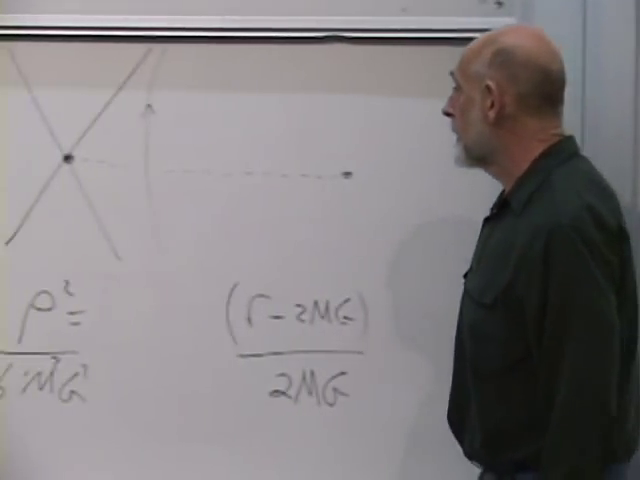
\includegraphics[width=0.72\textwidth]{lecture_03_figure_04.png}
\caption{近视界因果图板：交叉的零边界、外部楔形中的恒定半径双曲线，以及\(\rho\)与\(r-2GM\)之间的坐标关系。}
\lectureframe{00:34:35.000}
\end{figure}

\begin{figure}[htbp]
\centering
\begin{tikzpicture}[scale=1.04,>=Latex]
  \draw[->] (-0.3,0) -- (4.6,0) node[right] {\(X\)};
  \draw[->] (0,-3.2) -- (0,3.2) node[above] {\(T\)};
  \draw[very thick,blue!55!black] (0,0) -- (3,3);
  \draw[very thick,blue!55!black] (0,0) -- (3,-3);
  \node[blue!55!black,rotate=45] at (0.72,1.02) {future horizon};
  \draw[thick,domain=-1.45:1.45,samples=80] plot ({0.75*cosh(\x)},{0.75*sinh(\x)});
  \draw[thick,domain=-1.25:1.25,samples=80] plot ({1.25*cosh(\x)},{1.25*sinh(\x)});
  \draw[very thick,domain=-1.05:1.05,samples=80] plot ({2.0*cosh(\x)},{2.0*sinh(\x)});
  \node at (3.64,2.18) {Bob: \(\rho=\mathrm{const.}\)};
  \draw[very thick,red!65!black,->] (1.2,-2.9) -- (1.2,2.9);
  \node[red!65!black] at (1.58,-1.75) {Alice};
  \fill[red!65!black] (1.2,1.2) circle (1.7pt);
  \draw[dashed,->] (1.2,0) -- (2.27,1.07);
  \node[align=left] at (3.18,0.80) {\small pre-crossing\\[-0.2em]\small light signal};
\end{tikzpicture}
\caption{图板的排版配套图。鲍勃沿一条加速的恒定\(\rho\)双曲线运动；爱丽丝沿一条穿过未来视界的局部惯性线运动。零边界限制了鲍勃的因果可达范围，但并未成为爱丽丝的局部障碍。}
\end{figure}

\section{爱丽丝下落，鲍勃悬停}

让鲍勃保持与视界的固定距离，而爱丽丝松开他的手并下落。鲍勃的世界线是一条双曲线，因此是加速的。爱丽丝的局部世界线近似为直线。她在有限固有时间内穿过零边界，并且不会遇到任何局部不连续性。

因果描述是不对称的。Alice 穿越之后，来自她的光无法到达 Bob，而 Bob 发出的光在一段时间内仍能到达 Alice。Bob 接收到 Alice 在其有限下落入过程中越来越早阶段发出的信号。它们的到达时间间隔越拉越长，频率红移，强度衰减。在 Schwarzschild 时间中，他永远看不到穿越本身；Alice 看起来渐近地趋近并压扁在地平线上。并不是她的鼻子被压扁而后脑勺保持正常：来自每一部分的信号都被压缩进同一个极限层。

\begin{classroomqa}
\audiencequestion{Alice 穿越后能看到 Bob，是因为 Bob 的光子朝她向内传播吗？\lecturetimestamp{00:42:48}}
\lecturerresponse{是的。单向因果关系正是要点：Bob 的向内信号可以进入，而 Alice 后来的向外信号无法逃回 Bob。}
\end{classroomqa}

\begin{classroomqa}
\audiencequestion{如果 Alice 的脚先穿越而她的眼睛仍在外侧，她会暂时看不见自己的脚吗？\lecturetimestamp{00:43:03}}
\lecturerresponse{在普通下落过程中不会出现视觉上的中断。光从脚到眼睛总需要时间；等到相关信号到达时，她的眼睛也已经穿越了。只有猛烈地试图让她的头保持在外侧而脚继续向内，才会造成一种不同且具有破坏性的情形。}
\end{classroomqa}

保持位置是非惯性选择。Bob 需要火箭，正如站在地板上的人需要地板向上的力来避免自由下落。Bob 悬停得越靠近地平线，所需的固有加速度越大；在局部 Rindler 近似中，其大小为 \(a=1/\rho\)，单位为 \(c=1\)。\editorialnote{恢复单位后，对局部 Rindler 观察者给出 \(a=c^2/\rho\)。一个严格静态的 Schwarzschild 观察者的固有加速度在趋近地平线时发散。}

\begin{classroomqa}
\audiencequestion{我们站在报告厅里时是在加速吗？\lecturetimestamp{00:45:40}}
\lecturerresponse{是的，相对于自由下落参考系而言。地板支撑着我们；没有地板，或者没有喷气背包，我们就会下落。}
\end{classroomqa}

\begin{classroomqa}
\audiencequestion{Bob 最终能看到 Alice 位于地平线一个 Planck 长度之内吗？此后会发生什么？\lecturetimestamp{00:49:24}}
\lecturerresponse{正是在那里，经典几何描述不再充分。Planck 长度包含 \(\hbar\)，因此回答 Bob 在那里能分辨什么需要量子力学。}
\end{classroomqa}

\begin{classroomqa}
\audiencequestion{等半径曲线似乎以类似直角的坐标拐角与地平线相交。那里能取导数吗？\lecturetimestamp{00:51:12}}
\lecturerresponse{在这个点上，该坐标图确实发生了某种奇异的事情，但局部物理没有。覆盖其他楔区的坐标图会消除这个人为拐角。对于当前的外部讨论，Rindler 图像已经包含了所需的因果事实。}
\end{classroomqa}

因此，不指明观察者就问 Alice 是否\emph{真的}穿越了，是没有帮助的。Alice 的时钟在有限固有时间内到达地平线。Bob 接收到的信号序列从不包含穿越事件。物理学问的是每个观察者测量到什么，以及他们的记录如何比较。

\begin{classroomqa}
\audiencequestion{确切的陈述是 Bob 只能看到 Alice 未来的一有限部分，尽管他自己的观测时间无界吗？\lecturetimestamp{00:53:33}}
\lecturerresponse{是的。Alice 为她下落中可见的那部分分配了有限的固有时间。在理想化的永恒几何中，Bob 永远接收到其越来越延迟且红移的信号，但他看不到她在地平线穿越之后继续变老。}
\end{classroomqa}

\section{加速视界已经足够}

这一因果结构中没有任何东西需要黑洞。一个永远匀加速的火箭在平直时空中沿 Rindler 双曲线运动，并具有一个零边界，超过它任何信号都无法追上该火箭。对该观察者而言存在一个加速视界，尽管惯性观察者把同一区域视为普通的 Minkowski 空间。

\begin{classroomqa}
\audiencequestion{这一现象是黑洞特有的，还是对任何视界都会发生？\lecturetimestamp{00:55:25}}
\lecturerresponse{同一现象对匀加速观察者也会发生。这样的观察者有一个加速视界，看不到其外的事件。局部地看，黑洞视界与那种情形在物理上没有不同。}
\end{classroomqa}

这就是等效原理在起作用：先理解匀加速，然后在引力场中辨认出相同的局部结构。事后看来，甚至在黑洞被接受之前，人们本可以从加速视界预见到引力视界。爱因斯坦本人并不接受黑洞的物理形成，尽管正是他提供了其几何所由之导出的理论。视界对自由下落的观测者是乏味的，而对坚持留在外面的观测者则意义重大。这是两种有效描述之间的张力，尚不是悖论。

\section{回到热与熵}

休息之后，戴上热力学的帽子。在先前的构造中，黑洞像浴缸一样被一滴一滴地填满，只不过每一滴都是携带大约一个比特的光子。每个比特使视界面积增加一个普朗克面积量级的量。精确的熵为
\begin{equation}
S_{\mathrm{BH}}=\frac{k_B A}{4\ell_P^2}.
\end{equation}
讲座开玩笑说，如果普朗克当初以不同方式定义他的长度，因子\(1/4\)本可以避免。严肃的要点是，量纲分析确定了尺度，但没有确定数值系数；霍金的计算确定了系数。\editorialnote{普朗克长度有一个标准定义\(\ell_P=\sqrt{G\hbar/c^3}\)。一旦固定了这一约定和通常的热力学熵，因子\(1/4\)就是物理的；关于重新定义它的说法只是关于约定的课堂玩笑。}

温度感觉起来很基本，因为手指和温度计直接记录它。熵往往感觉更神秘。讲座颠倒了这一等级：熵和能量被当作基本变量，而温度则从熵变化时能量必须改变多少导出：
\begin{equation}
dE=T\,dS.
\end{equation}
在讲座的一个比特单位中，\(\Delta S=1\)，因此与增加或擦除一个比特相关的最小能量被称为\(T\)。粗心地擦除---用逻辑上相当于大锤的方式---可以耗散任意更多的能量。该定义关注的是当缺失的信息被转移到微观环境自由度中时可能的最小耗散。在常规单位中，一个二进制比特携带\(\Delta S=k_B\ln2\)，而可逆擦除至少耗散\(k_BT\ln2\)。\editorialnote{这就是讲座选择以基于能量的自然单位来测量熵和温度所压制的兰道尔归一化。}

\subsection{单光子估计}

选择一个波长与史瓦西半径相当的光子：
\begin{equation}
\lambda\sim R_s=\frac{2GM}{c^2}.
\end{equation}
在区分\(h\)与\(\hbar\)的\(2\pi\)约定下，其能量为
\begin{equation}
\Delta E\sim \frac{\hbar c}{\lambda}.
\end{equation}
这就是所增加比特的能量代价，所以
\begin{equation}
k_BT_H\sim\frac{\hbar c}{R_s}
\sim\frac{\hbar c^3}{GM}.
\label{eq:l03-hawking-scale}
\end{equation}
启发式论证无法确定诸如\(2\)和\(\pi\)这样的因子。精确的霍金结果是
\begin{equation}
\boxed{k_BT_H=\frac{\hbar c^3}{8\pi GM}.}
\label{eq:l03-hawking-exact}
\end{equation}

\begin{figure}[htbp]
\centering
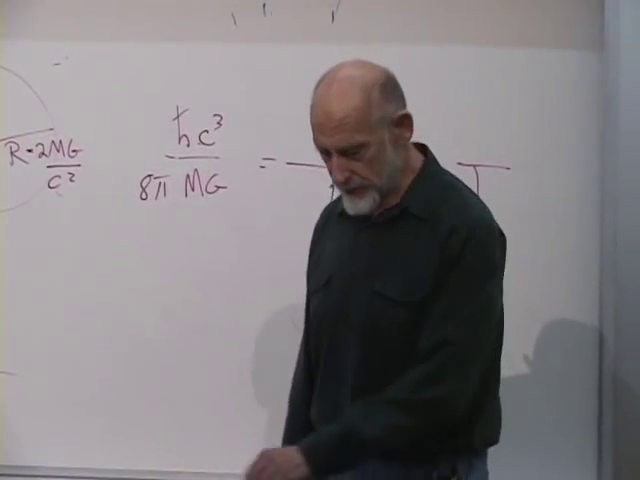
\includegraphics[width=0.72\textwidth]{lecture_03_figure_05.png}
\caption{完成的温度板书：\(R_s=2GM/c^2\)、一个比特尺度\(\hbar c/R_s\)，以及精确的\(8\pi\)霍金归一化。}
\lectureframe{01:07:48.000}
\end{figure}

两个事实立刻可见。第一，温度随\(\hbar\)而消失，所以它是一种量子效应。第二，
\begin{equation}
T_H\propto\frac{1}{M}.
\end{equation}
大黑洞是冷的。对于一个太阳质量，
\begin{equation}
T_H\approx6\times10^{-8}\ {\rm K},
\end{equation}
这与讲座的\(10^{-8}\,\mathrm{K}\)估计处于同一量级，并远低于约\(2.7\,\mathrm{K}\)的宇宙微波背景温度。

\subsection{负热容}

把这样的黑洞放入更暖的环境中。它吸收能量，质量增加，而方程~\eqref{eq:l03-hawking-exact}表明它变得更冷。于是它更容易继续吸收。把它放入更冷的环境中，则反向的失控开始：它辐射，失去质量，变得更热，并辐射得更快。形式上，
\begin{equation}
C_{\mathrm{BH}}
=\frac{dE}{dT_H}
=c^2\frac{dM}{dT_H}
<0.
\end{equation}

\begin{classroomqa}
\audiencequestion{这就是负比热的意思吗？\lecturetimestamp{01:14:08}}
\lecturerresponse{正是。一个自引力系统可以在失去能量时升温。恒星做类似的事情：当它辐射时，降低的压力使它收缩，而引力压缩提高其温度。}
\end{classroomqa}

孤立黑洞并不因此就是非物理的。在当今宇宙中，恒星级黑洞比其周围更冷，并主要吸收。随着宇宙膨胀和背景冷却，平衡最终可能反转，蒸发可能占主导。与有效无限热浴的简单平衡是不稳定的。\editorialnote{边界条件很重要。黑洞可以在有限反射腔中稳定下来，或者对于适当的大黑洞，在反德西特时空中稳定下来；这里描述的不稳定性是渐近平直、普通热浴的情形。}

\section{蒸发定律}

对于标度推导，设想手边没有参考书，选择使所记住的方程最为简洁的单位：
\begin{equation}
c=\hbar=G=k_B=1.
\end{equation}
这些就是普朗克单位。讲座中给出的特征尺度为
\begin{equation}
\ell_P\sim10^{-35}\ {\rm m},
\qquad
t_P\sim10^{-43}\ {\rm s},
\qquad
m_P\sim10^{-8}\ {\rm kg}.
\end{equation}
普朗克质量大致相当于一粒可见的尘埃，而普朗克长度和时间则极其微小。由于\(c=1\)，\(t_P\)不过是\(\ell_P\)的光穿越时间。

把黑洞视为黑体，即一个热辐射体，而不是一个必须保持完全黑暗的物体。它可以发射电磁辐射，原则上还可以发射其他可用的粒子种类，包括引力子。辐射功率与发射面积成正比，因为辐射是通过表面离开的。斯特藩--玻尔兹曼标度关系为
\begin{equation}
L=-\frac{dE}{dt}\sim A T^4.
\end{equation}
在普朗克单位下，\(E=M\)，\(R_s\sim M\)，\(A\sim R_s^2\sim M^2\)，\(T\sim R_s^{-1}\sim M^{-1}\)。因此
\begin{align}
-\frac{dM}{dt}
&\sim R_s^2\left(\frac{1}{R_s}\right)^4
\sim\frac{1}{R_s^2}
\sim\frac{1}{M^2},\\
-M^2\frac{dM}{dt}&\sim1,\\
-\frac{d(M^3)}{dt}&\sim1.
\label{eq:l03-evap-scaling}
\end{align}
忽略量级为1的系数，寿命为
\begin{equation}
\boxed{t_{\mathrm{evap}}\sim M^3.}
\label{eq:l03-lifetime}
\end{equation}

\begin{figure}[htbp]
\centering
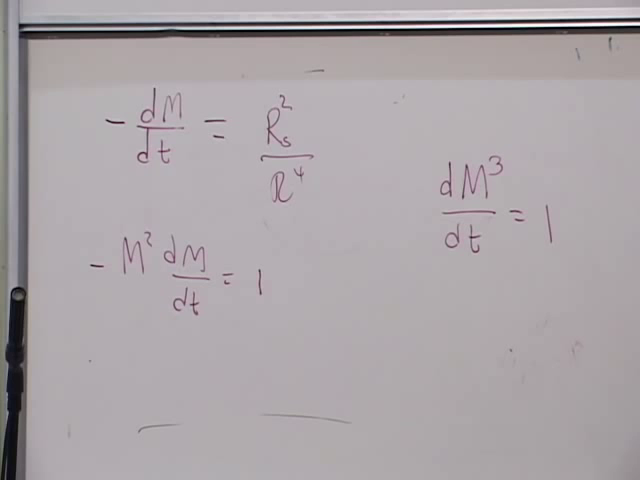
\includegraphics[width=0.72\textwidth]{lecture_03_figure_06.png}
\caption{畅通无阻的蒸发图景：光度给出\(-dM/dt\sim1/M^2\)，因此\(M^3\)均匀减小，寿命与初始质量的立方成正比。}
\lectureframe{01:23:20.000}
\end{figure}

这种示意性的斯特藩--玻尔兹曼处理忽略了灰体因子和粒子种类的数目。对于最简单的无质量发射近似下的中性、不转动黑洞，恢复常数后得到
\begin{equation}
t_{\mathrm{evap}}
=\frac{5120\pi G^2M_0^3}{\hbar c^4}.
\label{eq:l03-exact-lifetime}
\end{equation}
这个系数是编者补充的；讲座只推导稳健的\(M_0^3\)依赖关系。

\subsection{太阳、山岳与千克尺度}

太阳的质量为\(M_\odot\sim10^{30}\,\mathrm{kg}\sim10^{38}m_P\)。取立方并乘以一个普朗克时间，得到讲座中有意粗略的推导链
\begin{equation}
t_{\mathrm{evap}}\sim10^{114}t_P
\sim10^{71}\ {\rm s}
\sim10^{64}\ {\rm yr}.
\end{equation}
两种估计都比宇宙大约\(10^{10}\)年的年龄长得不可思议。恢复方程~\eqref{eq:l03-exact-lifetime}中的系数后，标准的太阳质量估计值提高到约\(2\times10^{67}\)年。\editorialnote{这一差异是意料之中的：黑板上的计算丢弃了所有数值常数，并将普朗克尺度按10的幂次取整。其目的是展示质量立方标度关系，而非精确的寿命天文学。}

接下来课堂上尝试了一个\emph{山岳质量}的黑洞。他们确定了粗略的课堂数值\(M\sim10^{10}\,\mathrm{kg}\)，因此\(M\sim10^{18}m_P\)，并得到
\begin{equation}
t_{\mathrm{evap}}\sim10^{54}t_P
\sim10^{11}\ {\rm s}
\sim10^4\ {\rm yr}.
\end{equation}
这保留了黑板上实际进行的算术。用来引出该质量的言语几何描述---大约\(100\,\mathrm{km}^3\)的岩石---实际上会重得多，而精确的寿命系数也会显著改变结果。\editorialnote{在普通岩石密度下，\(100\,\mathrm{km}^3\)的量级为\(10^{14}\,\mathrm{kg}\)，而非\(10^{10}\,\mathrm{kg}\)。对于\(10^{10}\,\mathrm{kg}\)，方程~\eqref{eq:l03-exact-lifetime}给出的寿命量级为\(10^6\)年。这些修正并不改变讲座的教训：寿命随质量的立方下降。}

\begin{classroomqa}
\audiencequestion{质量只有一千克的黑洞会极其微小吗？\lecturetimestamp{01:29:14}}
\lecturerresponse{是的。由于半径与质量成正比，而一个太阳质量对应几千米，所以一千克的黑洞的施瓦西半径约为\(10^{-27}\,\mathrm{m}\)。这样的黑洞也会极其炽热且寿命极短。}
\end{classroomqa}

\begin{classroomqa}
\audiencequestion{这些蒸发估计是否假设环境温度为零？\lecturetimestamp{01:29:53}}
\lecturerresponse{它们适用于周围环境比黑洞更冷、因而净能量向外流动的情形。更热的环境反而会向黑洞供给能量。霍金温度与当前背景温度相匹配的质量留作练习。}
\end{classroomqa}

为了便于定位，令\(T_H=2.7\,\mathrm{K}\)，得到\(M\)的量级为\(10^{22}\,\mathrm{kg}\)，施瓦西半径的量级为\(10^{-4}\,\mathrm{m}\)。\editorialnote{这是对讲座中所提练习的解答；它不属于口头推导的一部分。}

\section{度规之下必须有什么？}

\begin{classroomqa}
\audiencequestion{是什么机制使光子从黑洞中出来？\lecturetimestamp{01:30:53}}
\lecturerresponse{在给出辐射的微观机制之前，必须先确定负责熵的自由度。热力学论证约束了必须存在什么，但尚未明确展示那些变量。}
\end{classroomqa}

类比是流体力学。流体动力学描述光滑的密度场和速度场，而不追踪每一个分子。然而熵揭示出，许多隐藏的微观组态构成了同一个光滑状态的基础。同样地，经典广义相对论描述光滑的度规，却不暴露黑洞熵所计数的众多微观自由度。面积定律和霍金辐射是线索，表明爱因斯坦的理论是一种有效的宏观描述。

\begin{classroomqa}
\audiencequestion{如果黑洞辐射能量，这是否等同于说它辐射信息，从而在增长过程中被吞入的信息会在蒸发过程中返回？\lecturetimestamp{01:33:27}}
\lecturerresponse{这正是要求所在：如果完整的演化守恒信息，那么出射辐射最终必须能够区分形成该黑洞的各种可能状态。这仍须与物质穿过视界的因果图像相协调。}
\end{classroomqa}

仅凭能量通量不足以确定信息。一个完全热化的密度矩阵可以携带能量，却遗忘详细的初始状态。在幺正描述中，所需的信息编码于发射量子之间的精细关联之中。\editorialnote{这一区分明确揭示了信息问题的现代形式。它使讲座中提出的问题更加尖锐，而非改变该问题。}

\section{信息守恒作为结构性原理}

\begin{classroomqa}
\audiencequestion{信息守恒真的是一条基本原理吗？\lecturetimestamp{01:34:13}}
\lecturerresponse{它属于最根本的原理之列。如果不同的初始状态能够演化到完全相同的末态，那么定律就会抹去自身的过去。通常的守恒定律不仅依赖于对称性，还依赖于可逆的哈密顿量或幺正形式的演化。}
\end{classroomqa}

如讲座中那样，设想一条虚构的基本定律，它只是让每一块滑动的橡皮都停下来。不同的初始速度最终都终结于同一状态。末态的橡皮不再能区分它的历史：信息已被摧毁。动量和机械能也一并消失。真实的摩擦在微观层面并不会如此；动量和能量会传入桌面、空气和热自由度之中。

即便是一个完全均匀的无限大桌面，也会具有平移对称性，然而那条虚构的阻尼定律仍能使橡皮停下。因此，仅凭平移对称性并不足以从这样一条非哈密顿规则导出动量守恒。诺特定理假定了一个作用量原理以及与之相关的可逆动力学。用这里使用的语言来说，对称性加上保信息的动力学才给出守恒定律。

\begin{classroomqa}
\audiencequestion{信息守恒比因果性更根本吗？\lecturetimestamp{01:37:00}}
\lecturerresponse{它们是处于相当的基础层面上的不同原理。因果性必须首先被精确陈述---例如，信号不能逆着传播到允许的因果结构之外---但这两个原理都不能简单地取代另一个。}
\end{classroomqa}

\begin{classroomqa}
\audiencequestion{哈密顿力学中讨论的相空间面积保持，是这一思想的经典版本吗？\lecturetimestamp{01:37:38}}
\lecturerresponse{是的。刘维尔定理说，哈密顿流保持相空间体积。一团可能的初始状态不能坍缩到更小的体积中并抹去区分。在量子力学中，相应的陈述是幺正性：内积，从而正交状态之间的区分，都得到保持。}
\end{classroomqa}

经典地，
\begin{equation}
\frac{d}{dt}\,\mathrm{Vol}_{\Gamma}=0,
\end{equation}
对于由哈密顿流输运的相空间区域。量子力学地，
\begin{equation}
\begin{aligned}
\ket{\psi(t)}&=U(t)\ket{\psi(0)},\\
U^\dagger U&=I,\\
\braket{\psi(t)}{\phi(t)}
&=\braket{\psi(0)}{\phi(0)}.
\end{aligned}
\end{equation}
这些是“微观区分在时间演化中得以存留”这一主张的精确形式。

\section{熵依赖于哪个方向？}

最后的交流回到信息论熵。给定微观备选情形的概率\(p_i\)，
\begin{equation}
S=-k_B\sum_i p_i\ln p_i
\label{eq:l03-shannon}
\end{equation}
以热力学单位表示，或者去掉\(k_B\)后得到无量纲的香农熵。

\begin{figure}[htbp]
\centering
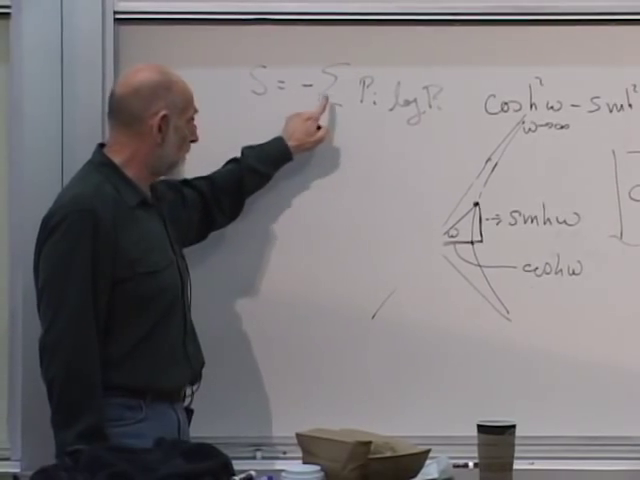
\includegraphics[width=0.72\textwidth]{lecture_03_figure_07.png}
\caption{结尾的板书公式\(S=-\sum_i p_i\log p_i\)，书写时区分了概率分布与由它计算出的单个熵值。}
\lectureframe{01:40:32.000}
\end{figure}

\begin{classroomqa}
\audiencequestion{是最大化熵定义了概率分布，而不是概率定义了熵吗？\lecturetimestamp{01:38:33}}
\lecturerresponse{一个概率分布通过式~\eqref{eq:l03-shannon}确定一个熵值；一个数无法重构所有的\(p_i\)。只有在归一化以及其他约束，例如固定的平均能量，也已被给出之后，最大化熵才能选出一个分布。}
\end{classroomqa}

这一区分使讲座恰好在正确的前沿结束。光滑几何引出了视界；视界引出了热力学；热力学暴露了隐藏的自由度；而信息守恒现在要求这些自由度在演化时不抹去进入黑洞的那些区分。机制尚未给出。相反，几何与记账已经清楚表明，任何成功的微观理论都必须解释什么。

\chapter{黑洞、白洞与整体因果图}

\lectureoverview{视界在局部是普通的，在整体上却是决定性的。我们从近视界施瓦西度规出发，借助欧几里得雪茄的类比向外推进，然后追问爱丽丝和鲍勃实际上能看到什么。奇点以及时间反演的白洞区域把这一局部图像扩展为永恒的施瓦西时空。彭罗斯紧致化使因果结构变得有限而可读。最后一步则从永恒解转向由坍缩形成的黑洞，其中牛顿球壳定理和伯克霍夫定理提供了需要拼接起来的各个部分。}

\section{从视界到无穷远}

在足够大的施瓦西视界附近，曲率在一个小实验室范围内是弱的，径向-时间几何近似为平坦的。方便的径向变量不是施瓦西坐标\(r\)，而是沿等时空间切片从视界向外测量的固有距离\(\rho\)：
\begin{equation}
\rho=0 \quad\Longleftrightarrow\quad r=2GM .
\label{eq:l04-rho-horizon}
\end{equation}
方便的时间坐标是无量纲量
\begin{equation}
\omega=\frac{t}{4GM},
\label{eq:l04-omega}
\end{equation}
其中\(c=1\)。因此，\(\omega\)是以两倍施瓦西半径为单位的施瓦西时间。

在mostly-plus约定下，近视界径向-时间度规为
\begin{equation}
ds^2\approx-\rho^2d\omega^2+d\rho^2.
\label{eq:l04-rindler}
\end{equation}
角向二维球面已被略去，因为当前的论证只涉及时间和径向距离。

\begin{figure}[htbp]
\centering
\includegraphics[width=0.72\textwidth]{lecture_04_figure_02.png}
\caption{近视界度规与重新标度的施瓦西时间。}
\lectureframe{00:05:46.800}
\end{figure}

方程~\eqref{eq:l04-rindler}与闵可夫斯基时空的关系，正如极坐标与欧几里得平面的关系。对于
\begin{equation}
T=\rho\sinh\omega,
\qquad
X=\rho\cosh\omega,
\end{equation}
可得
\begin{equation}
-dT^2+dX^2=-\rho^2d\omega^2+d\rho^2.
\end{equation}
常数\(\rho\)的线是双曲线\(X^2-T^2=\rho^2\)，而\(\omega\)从遥远的过去延伸到遥远的未来。两条零线\(X=\pm T\)在约化图的分叉点相交。在四维中，该点代表一个二维球面，而未来和过去的零面构成分叉的基灵视界。\editorialnote{只把交点称为分叉视界，在径向图中是有用的简略说法。更确切地说，两支视界分支相交于一个分叉二维球面。}

\subsection{远处区域}

施瓦西度规的径向-时间部分为
\begin{equation}
ds^2
=-\left(1-\frac{2GM}{r}\right)dt^2
+\frac{dr^2}{1-\frac{2GM}{r}}.
\label{eq:l04-schwarzschild}
\end{equation}
远离黑洞处，\(r\gg2GM\)，度规趋近于
\begin{equation}
ds^2\approx-dt^2+dr^2.
\end{equation}
在那里，\(r\)与\(\rho\)只相差一个无关紧要的加性修正，因此取\(dt=4GM\,d\omega\)，
\begin{equation}
ds^2\approx-(4GM)^2d\omega^2+d\rho^2.
\label{eq:l04-far}
\end{equation}
径向系数在两个极限下都很简单。发生变化的是时间系数：
\begin{equation}
ds^2\approx
\begin{cases}
-\rho^2d\omega^2+d\rho^2, & \rho\ll GM,\\[3pt]
-(4GM)^2d\omega^2+d\rho^2, & \rho\gg GM.
\end{cases}
\label{eq:l04-two-limits}
\end{equation}
沿悬停轨迹，\(d\rho=0\)。靠近视界处，
\begin{equation}
d\tau=\rho\,d\omega,
\end{equation}
而在远处\(d\tau\approx4GM\,d\omega=dt\)。对于外部时间坐标的固定增量，越靠近视界被保持的时钟所经历的固有时间越少。

\subsection{雪茄}

时空难以想象，因此把类时方向替换为普通的角方向。写
\begin{equation}
\begin{aligned}
d\ell^2&=F(\rho)^2d\theta^2+d\rho^2,\\
F(\rho)&\sim
\begin{cases}
\rho, & \rho\to0,\\
4GM, & \rho\to\infty.
\end{cases}
\end{aligned}
\label{eq:l04-cigar}
\end{equation}
在\(\rho=0\)附近，这就是极坐标中的平面。在远处，周长不再随半径增长：
\begin{equation}
C_\infty=\int_0^{2\pi}4GM\,d\theta=8\pi GM.
\label{eq:l04-cigar-circumference}
\end{equation}
因此该曲面在一端圆滑收拢，在另一端趋近于圆柱面。它看起来像一支雪茄。

\begin{figure}[htbp]
\centering
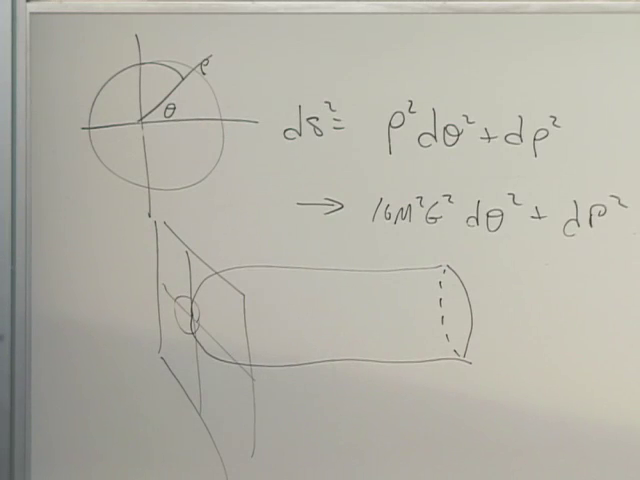
\includegraphics[width=0.74\textwidth]{lecture_04_figure_03.png}
\caption{欧几里得类比：一个极坐标尖端连接到一个周长为\(8\pi GM\)的渐近圆柱面。}
\lectureframe{00:14:05.000}
\end{figure}

质量越大，渐近处的围长越大，尖端附近的弯曲越平缓。小黑洞对应弯曲得很紧的雪茄；大黑洞则有一个宽阔、弯曲很弱的尖端。这是方程~\eqref{eq:l04-two-limits}中插值的图像，而不是洛伦兹黑洞本身的嵌入。\editorialnote{精确的几何对象是通过将施瓦西时间延拓到虚时间而得到的。于是尖端处的光滑性把欧几里得时间周期固定为\(8\pi GM\)，这同一个尺度后来决定了霍金温度。本讲在此只使用视觉类比。}

\section{从因果角度解读视界}

在黑洞外部，\(\rho>0\)，静止观测者沿一条常数\(\rho\)的双曲线运动。在远处，只需适度的加速度就能抵抗引力；靠近视界处，所需的固有加速度无界增长。一旦某条世界线穿过未来零边界，来自它的任何未来指向的因果信号都无法到达外部。

\begin{classroomqa}
\audiencequestion{在这个图上，光线是直线吗？\lecturetimestamp{00:20:21}}
\lecturerresponse{径向光线画在\(45^\circ\)处，除非另有约定。入射光线穿过视界；而已经在内部的出射光线无法再穿回外部。}
\end{classroomqa}

\begin{classroomqa}
\audiencequestion{入射光线会停留在视界上吗？\lecturetimestamp{00:21:12}}
\lecturerresponse{不会。向内瞄准的光线会穿过未来视界并继续进入黑洞内部。只有视界生成元本身才停留在零边界上。}
\end{classroomqa}

\subsection{Bob观察Alice}

让Bob在外部固定半径处悬停，而Alice向内下落。Bob只有通过接收来自Alice的向外传播的光才能看到她。假设她按照自己的时钟周期性地挥手。在她下落过程中较晚发出的信号需要越来越长的Schwarzschild时间才能到达Bob，而他每单位时间接收到的波越来越少。在穿过视界之后发出的任何信号都无法返回他那里。

Rindler坐标揭示了极限行为。定义出射零坐标
\begin{equation}
U=T-X=-\rho e^{-\omega}.
\end{equation}
趋近未来视界意味着\(U\to0^{-}\)，这要求在固定的外部\(\rho\)下\(\omega\to+\infty\)。因此，对Alice而言有限的穿越事件被推到了无限的外部时间。相继的波峰以指数增长的间隔到达，因此其频率被指数红移。\editorialnote{这一零坐标计算给出了课堂上定性描述的红移的数学形式。它只使用了局部Rindler近似。}

起初Bob接收到可见光，然后是红外线，接着是波长极大的无线电波。有用的陈述并不是Alice作为一张永久可见的照片停留在视界上。她变得更暗、更红，最终无法探测。

\begin{classroomqa}
\audiencequestion{Bob会看到Alice冻结在视界外某个确切位置吗？\lecturetimestamp{00:26:31}}
\lecturerresponse{在经典的外部坐标描述中，在越来越晚的时间接收到的图像来自越来越靠近视界的事件。极限图像冻结在那里，但其辐射被红移到实际上消失。量子黑洞物理尚未进入这一叙述。}
\end{classroomqa}

\begin{classroomqa}
\audiencequestion{当Alice逐渐消失时，她看起来也被压缩了吗？\lecturetimestamp{00:28:34}}
\lecturerresponse{是的。相对运动在外部描述中产生纵向Lorentz收缩。这里重要的观测效应仍然是红移：她的内部振荡显得更慢，接收到的波长增大。}
\end{classroomqa}

\subsection{Alice观察Bob}

Alice的固有时在视界处保持规则。她在穿过之后继续接收来自Bob的向内传播的信号，因为这些信号遵循与她相同的因果方向。一旦她进入内部，就无法回复外部。视界是单向的，而不是从两侧对称地遇到的墙。

\begin{classroomqa}
\audiencequestion{Alice穿过视界下落时，会看到Bob的光发生蓝移吗？\lecturetimestamp{00:30:29}}
\lecturerresponse{在所使用的图像中，她看到Bob在退行，其信号向红端移动；在她的穿越处没有奇异现象发生。精确的频率移动取决于两条世界线以及Bob何时发出信号，因此不变性的陈述是：在规则视界处她测得的频率保持有限。}
\end{classroomqa}

\begin{classroomqa}
\audiencequestion{同样的因果限制适用于引力子吗？\lecturetimestamp{00:31:15}}
\lecturerresponse{它适用于真正的引力辐射，正如它适用于光子一样。从未来视界后方发出的任何辐射扰动都无法到达Bob。}
\end{classroomqa}

\begin{classroomqa}
\audiencequestion{当Alice落入时，她的能量会增加黑洞的质量和半径吗？\lecturetimestamp{00:31:43}}
\lecturerresponse{是的。一旦她的能量被纳入黑洞，其质量上升，其Schwarzschild半径\(R_s=2GM\)也随之上升。动力学形成问题将使这一陈述几何化。}
\end{classroomqa}

\subsection{为什么外部仍然有引力}

黑洞是暗的，但并非没有引力。静态引力场不是从内部不断逃逸的壳上引力子流。它是已经建立起来的外部几何。如果源发生变化，场的变化会以因果方式传播；远处的观察者不可能在光信号能够到达之前探测到该变化。

\begin{classroomqa}
\audiencequestion{如果引力子无法逃逸，为什么黑洞仍然施加引力？\lecturetimestamp{00:32:04}}
\lecturerresponse{静态场已经存在于外部。人们可以宽松地用虚引力子来描述它，但那些不是从内部携带新信息的可探测粒子。受光速限制的是场的变化，包括引力辐射。}
\end{classroomqa}

\begin{classroomqa}
\audiencequestion{虚拟引力子如何能与场的变化以光速传播这一说法相协调？\lecturetimestamp{00:34:02}}
\lecturerresponse{虚拟量子是微扰计算中的记账要素，而不是具有可测量轨迹的携带信号的粒子。规范不变的扰动和信息按因果方式传播。静态电磁场与电磁辐射之间也出现同样的区分。}
\end{classroomqa}

因此，关于虚拟引力子可以超过光速的课堂说法不应被理解为超光速通信。\editorialnote{离壳的虚拟粒子不必满足在壳色散关系，但它们不是可观测量，也不能用来传递信息。在广义相对论中，清晰的描述更为简单：静态的外部度规存在，而引力场的变化具有因果传播。}

\section{爱丽丝还能看到她的脚吗？}

让爱丽丝脚朝下下落。她的脚先于她的头穿过视界。当她向下看时，她永远不会看到脚的世界线上同时发生的事件；光需要时间传播，所以她看到的是稍早一些的事件上的脚。在她的头穿过之前和之后，都存在这样一系列连续过去的事件。仅仅因为她身体的一部分已经越过\(r=2GM\)，局部并不会发生任何不连续的事情。

危险的实验是在脚已经进入之后反转方向。为了让头留在外面，爱丽丝必须向外加速。她的脚已经越过了未来视界，无法沿着外部悬停的轨迹运动。在加速参考系中，两者之间的间隔无界增长，而一个物质体无法跨越那条因果边界保持刚性。她要么与她的脚一起自由下落，要么在试图将自己其余部分保持在外部时被撕裂。

这种拉伸并不是大视界处发散的潮汐力。它是要求一个延展物体遵循互不相容的世界线所带来的后果。\editorialnote{足够大的史瓦西视界具有很小的潮汐曲率。这个思想实验中的病态来自所尝试的加速和刚性约束，而不是来自视界处的局部曲率奇点。}

\section{奇点在未来}

回到方程~\eqref{eq:l04-schwarzschild}。在外部，
\begin{equation}
1-\frac{2GM}{r}>0,
\end{equation}
所以在史瓦西坐标中\(t\)是类时的，而\(r\)是类空的。在内部，
\begin{equation}
1-\frac{2GM}{r}<0,
\end{equation}
这些坐标的角色反转：减小的\(r\)是一个类时方向。这并不意味着空间在视界处物理上变成了时间。它意味着史瓦西图在那里退化，并且其标签在内部具有不同的因果性质。

真正的奇点在
\begin{equation}
r=0.
\end{equation}
它并不是一条代表某个可以避开的地点的竖直世界线。它是一个类空的未来边界。一旦爱丽丝进入黑洞区域，每一条未来指向的类时或类光路径都在那里终结。曲率不变量
\begin{equation}
R_{\mu\nu\rho\sigma}R^{\mu\nu\rho\sigma}
=\frac{48G^2M^2}{r^6}
\label{eq:l04-kretschmann}
\end{equation}
在\(r\to0\)时发散，而在\(r=2GM\)处则是有限的。\editorialnote{方程~\eqref{eq:l04-kretschmann}是标准的史瓦西克雷奇曼标量。它使讲座中在几何上区分的规则视界与曲率奇点之间的区别成为不变量。}

\section{时间反演与白洞}

史瓦西度规与\(t\)无关，而\(dt^2\)在\(t\mapsto-t\)下不变。因此它的最大延拓在时间反演下是对称的。除了未来奇点和未来视界之外，这个数学解还包含一个过去奇点和一个过去视界。

将爱丽丝的下落进行时间反演。她现在从过去奇点中出现，向外穿过过去视界，并出现在鲍勃的外部。那个区域被称为白洞。它不是从未来黑洞内部逃出的路径：未来视界和过去视界是不同的类光边界。

\begin{classroomqa}
\audiencequestion{如果爱丽丝不能向外穿过黑洞视界，那么反演后的爱丽丝怎么能出来？\lecturetimestamp{00:50:24}}
\lecturerresponse{她并不是向外穿过未来视界。她向外穿过的是过去视界，正好是普通落入的时间反演。未来黑洞区域仍然没有向外的因果路径。}
\end{classroomqa}

\begin{classroomqa}
\audiencequestion{在白洞图像中，鲍勃的整个历史也必须被反向运行吗？\lecturetimestamp{00:52:15}}
\lecturerresponse{不。延拓几何允许这样一种历史：鲍勃留在外部，而爱丽丝从过去视界中出现。这个疑难不在于数学上的一致性；而在于过去奇点所代表的非同寻常的初始条件。}
\end{classroomqa}

\begin{figure}[htbp]
\centering
\includegraphics[width=0.72\textwidth]{lecture_04_figure_04.png}
\caption{讨论过程中逐步绘制的因果草图：交叉的视界、未来与过去的奇点曲线，以及观察者的轨迹。}
\lectureframe{01:00:19.818}
\end{figure}

\begin{figure}[htbp]
\centering
\begin{tikzpicture}[scale=0.92]
\draw[blue!75!black,thick] (-3,-3) -- (3,3);
\draw[blue!75!black,thick] (-3,3) -- (3,-3);
\draw[very thick,decorate,decoration={snake,amplitude=1.4pt,segment length=7pt}]
  (-2.55,2.75) .. controls (-1.45,1.35) and (1.45,1.35) .. (2.55,2.75);
\draw[very thick,decorate,decoration={snake,amplitude=1.4pt,segment length=7pt}]
  (-2.55,-2.75) .. controls (-1.45,-1.35) and (1.45,-1.35) .. (2.55,-2.75);
\draw (0.75,-2.75) .. controls (1.55,-1.15) and (1.55,1.15) .. (0.75,2.75);
\draw (1.55,-2.75) .. controls (2.35,-1.15) and (2.35,1.15) .. (1.55,2.75);
\draw[red!75!black,very thick] (2.6,-2.0) .. controls (1.65,-0.9) and (0.75,0.2) .. (0.2,1.55);
\fill (0,0) circle (1.5pt);
\node[above,font=\small] at (0,1.95) {future singularity};
\node[below,font=\small] at (0,-1.95) {past singularity};
\node[right] at (2.10,0.65) {exterior};
\node[left] at (-2.10,0.65) {second exterior};
\node[font=\scriptsize] at (-0.35,1.15) {black hole};
\node[font=\scriptsize] at (-0.35,-1.15) {white hole};
\node[font=\small,anchor=east] (bifurcation-label) at (-0.35,-0.15) {bifurcation};
\draw[->,thin] (bifurcation-label.east) -- (0,0);
\end{tikzpicture}
\caption{经过整理的未紧致化因果图。零测地视界在分叉面上相交；类空奇点位于未来与过去的楔形区域内。}
\end{figure}

\subsection{可能并不等于典型}

微观力学在极好的近似下具有时间反演不变性，然而宏观历史却有一个优先的方向。炸弹很容易爆炸；散落的碎片几乎从不会重新聚拢来把它重建起来。球很容易从一个不稳定的顶点滚下；一个随机抛出的球几乎从不会恰好停在那里。摆成三角形的台球很容易散开，而散开的球不会自发地排列成球架。冰块在热水中融化，而水几乎从不会吐出一个新组装好的冰块。

区别在于熵。低熵宏观态只占据相空间中极小的区域；高熵宏观态则包含数量巨大的微观排列。方程允许反向的轨迹，但要制备其初始微观态需要极其精确的关联。

\begin{classroomqa}
\audiencequestion{难道每一个精确的散射构型不都与精确的时间反演构型同样不可能吗？\lecturetimestamp{00:56:55}}
\lecturerresponse{对于逐个指定的微观态而言，是的。当我们比较宏观态时，不对称性才出现。一个散射的排列所包含的微观态远多于一个精确组装好的三角形，因此几乎每一个与第一种描述相容的微观态在宏观上仍然是无序的。}
\end{classroomqa}

一个发射出完全组织化的Alice的白洞，就是这种降低熵的历史在引力上的版本。可逆方程允许它，但它需要一个极其特殊的过去。视界本身携带熵和隐藏的微观信息，因此一个Alice大小的涨落并非逻辑上被禁止；它只是被压倒性地抑制了。

\begin{classroomqa}
\audiencequestion{这样的涨落是量子力学的还是热学的？\lecturetimestamp{00:59:48}}
\lecturerresponse{两种都可以有贡献。在普通的热系统中，主导的语言是热涨落；对于黑洞，量子效应与热效应交织在一起。无论哪种情况，核心的抑制都是熵性的。}
\end{classroomqa}

\section{固有距离与Penrose紧致化}

在绘制整体时空之前，我们应当把径向的术语精确化。固有时是时钟沿类时世界线所测量的量。固有距离是一系列局域米尺沿选定的类空曲线所测量的量。对于Schwarzschild的常\(t\)切片，
\begin{equation}
d\rho=\frac{dr}{\sqrt{1-2GM/r}}.
\label{eq:l04-proper-distance}
\end{equation}
因此\(r\)是一个面积坐标，而不是从视界出发的直接米尺距离。

现在从径向平直时空开始。只保留\(t\)和\(\rho\ge0\)。线\(\rho=0\)是空间原点，一条进入原点的径向光线在相反的一侧物理上继续向外传播，这在约化半平面中表现为一次反射。

Penrose图把\(t\)和\(\rho\)的所有有限与无限取值映射到一个有限区域，同时保持零方向。它的两条规则是：
\begin{enumerate}
\item 把整个时空紧致化到一个有限区域；
\item 保持径向光线在\(45^\circ\)。
\end{enumerate}
长度和普通角度被扭曲；因果关系则不然。

\begin{figure}[htbp]
\centering
\includegraphics[width=0.70\textwidth]{lecture_04_figure_06.png}
\caption{径向Minkowski时空的完整紧致化网格。无限时间位于左上和左下的端点，无限半径被压缩到右侧的尖端。}
\lectureframe{01:14:44.040}
\end{figure}

\begin{figure}[htbp]
\centering
\begin{tikzpicture}[scale=0.92]
\coordinate (im) at (0,-3);
\coordinate (ip) at (0,3);
\coordinate (iz) at (3,0);
\draw[very thick] (im) -- (ip) -- (iz) -- cycle;
\draw[gray] (0,-2.1) .. controls (0.8,-1.15) and (1.8,-0.35) .. (2.65,0);
\draw[gray] (0,-1.05) .. controls (0.9,-0.6) and (1.9,-0.15) .. (2.65,0);
\draw[gray] (0,0) -- (2.65,0);
\draw[gray] (0,1.05) .. controls (0.9,0.6) and (1.9,0.15) .. (2.65,0);
\draw[gray] (0,2.1) .. controls (0.8,1.15) and (1.8,0.35) .. (2.65,0);
\draw[gray] (0.65,-2.55) .. controls (1.0,-0.9) and (1.0,0.9) .. (0.65,2.55);
\draw[gray] (1.25,-1.75) .. controls (1.7,-0.7) and (1.7,0.7) .. (1.25,1.75);
\draw[gray] (1.95,-1.05) .. controls (2.25,-0.4) and (2.25,0.4) .. (1.95,1.05);
\draw[red!75!black,thick] (1.5,-1.5) -- (0,0) -- (1.5,1.5);
\node[left] at (ip) {\(i^+\)};
\node[left] at (im) {\(i^-\)};
\node[right] at (iz) {\(i^0\)};
\node[above right] at (1.35,1.65) {\(\mathcal{I}^+\)};
\node[below right] at (1.35,-1.65) {\(\mathcal{I}^-\)};
\node[left] at (0,0) {\(\rho=0\)};
\end{tikzpicture}
\caption{有限三角形中的径向Minkowski时空。红色光线从\(\mathcal{I}^-\)进入，到达原点，并从\(\mathcal{I}^+\)离开。}
\label{fig:l04-flat-penrose}
\end{figure}

这些端点具有不同的因果含义：
\begin{equation}
\begin{aligned}
i^-&:\ \text{past timelike infinity},\\
i^+&:\ \text{future timelike infinity},\\
i^0&:\ \text{spatial infinity},\\
\mathcal{I}^-&:\ \text{past null infinity},\\
\mathcal{I}^+&:\ \text{future null infinity}.
\end{aligned}
\end{equation}
符号\(\mathcal{I}^{-}\)和\(\mathcal{I}^{+}\)读作scri minus和scri plus。

\begin{classroomqa}
\audiencequestion{光线是否应当穿过每个被扭曲的网格单元的角点，从而略微弯曲？\lecturetimestamp{01:11:08}}
\lecturerresponse{如果完整地画出坐标网格，其交点会与零曲线一致。关键的构造是共形的：径向零方向保持在\(45^\circ\)，尽管常\(t\)和常\(\rho\)的网格线会弯曲并变得密集。}
\end{classroomqa}

\begin{classroomqa}
\audiencequestion{如果光线没有射向原点，该如何绘制它？\lecturetimestamp{01:11:45}}
\lecturerresponse{它会到达一个非零的最近接近距离，然后向外返回。一旦保留了角向运动，其投影的径向路径就不必是一条单一的直线\(45^\circ\)。}
\end{classroomqa}

\begin{classroomqa}
\audiencequestion{那么为什么那条光线不在\(45^\circ\)处？\lecturetimestamp{01:12:49}}
\lecturerresponse{\(45^\circ\)规则是针对径向光线陈述的。携带角动量的零测地线将其部分运动用于角方向，因此它在\(t\)-\(\rho\)平面上的投影不是径向的。}
\end{classroomqa}

\section{永恒史瓦西图}

紧致化后的图有四个区域。其两侧的菱形是渐近平直的外部区域。上方的三角形是黑洞内部，终止于未来类空奇点。下方的三角形是白洞区域，起始于过去类空奇点。这些区域共同构成了最大延拓的史瓦西几何。

\begin{figure}[htbp]
\centering
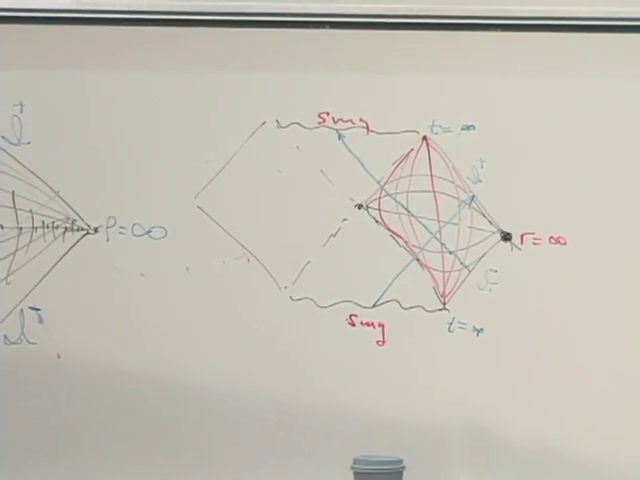
\includegraphics[width=0.74\textwidth]{lecture_04_figure_07.png}
\caption{黑板上画出的完整永恒史瓦西彭罗斯图，标有奇点、视界、零测地线以及一个渐近边界。}
\lectureframe{01:21:30.000}
\end{figure}

\begin{figure}[htbp]
\centering
\begin{tikzpicture}[scale=0.90]
\coordinate (C) at (0,0);
\coordinate (TL) at (-2,2);
\coordinate (TR) at (2,2);
\coordinate (BL) at (-2,-2);
\coordinate (BR) at (2,-2);
\coordinate (L) at (-4.0,0);
\coordinate (R) at (4.0,0);
\draw[very thick] (TL) -- (TR);
\draw[very thick] (BL) -- (BR);
\draw[thick] (C) -- (TL) (C) -- (TR) (C) -- (BL) (C) -- (BR);
\draw[thick] (TL) -- (L) -- (BL);
\draw[thick] (TR) -- (R) -- (BR);
\draw[red!75!black,very thick] (3,-1) -- (1,1) -- (0,2);
\node[above] at (0,2) {\(r=0\), future singularity};
\node[below] at (0,-2) {\(r=0\), past singularity};
\node[font=\small] at (0,1.15) {black hole};
\node[font=\small] at (0,-1.15) {white hole};
\node at (2.4,0.45) {Bob's exterior};
\node at (-2.4,0.45) {second exterior};
\node[right] at (R) {\(i^0_R\)};
\node[left] at (L) {\(i^0_L\)};
\fill (C) circle (1.5pt);
\end{tikzpicture}
\caption{永恒史瓦西的四个区域。一条入射径向光线穿过未来视界并终止于\(r=0\)。}
\label{fig:l04-eternal}
\end{figure}

一条来自\(\mathcal{I}^-\)的入射径向光线穿过未来视界并终止于奇点。上方三角形中的每一条因果曲线都有同样的命运。第二个外部区域常被描述为爱因斯坦--罗森桥的另一端开口，但它不可穿越：任何从一个外部区域到另一个外部区域的因果旅行尝试都会进入黑洞区域并到达奇点。

\begin{classroomqa}
\audiencequestion{两个外部世界是否由虫洞连接，能否通过它发送信号？\lecturetimestamp{01:22:21}}
\lecturerresponse{永恒几何在适当的空间切片上包含一个爱因斯坦--罗森桥，但没有因果信号能从一个外部区域穿越到另一个外部区域。桥收缩得太快；甚至进入视界的光也会终止于未来奇点。}
\end{classroomqa}

这张图描述的是一个自始至终存在的洞。真实的的天体物理黑洞由坍缩物质形成。它们的因果图没有过去的白洞奇点，也没有第二个渐近外部区域。要构造那种几何，我们需要理解球壳。

\section{通过坍缩制备黑洞}

想象一个由入射粒子组成的弥散球壳。它们可以是光子：能量产生引力，因此足够集中的辐射脉冲可以形成黑洞。坍缩之前，中心区域类似于空的平直时空；在足够能量被压缩之后，外部区域类似于史瓦西。任务是在移动的球壳两侧衔接这些区域。

\subsection{牛顿球壳定理}

对于总质量为\(M\)的球对称牛顿球壳，引力的高斯定律为
\begin{equation}
\oint \mathbf{g}\cdot d\mathbf{A}=-4\pi G M_{\mathrm{enc}}.
\label{eq:l04-gauss-gravity}
\end{equation}
球对称性使得\(\mathbf{g}=g(r)\hat{\mathbf r}\)，因此
\begin{equation}
g(r)=
\begin{cases}
0, & r<R_{\mathrm{shell}},\\[4pt]
-\dfrac{GM}{r^2}, & r>R_{\mathrm{shell}}.
\end{cases}
\label{eq:l04-shell-field}
\end{equation}
在内部，没有质量被包围，引力场消失。在外部，球壳的作用完全等同于位于中心的点质量\(M\)。内部的势是常数而非零，但不再存在局部牛顿力。\editorialnote{课堂上给出的场线论证被高斯定律精确地捕捉。零场与常数势之间的区别在比较相对论中的时钟归一化时很重要。}

只要总质量守恒，当一个完美球对称的球壳收缩时，该结论仍然成立。只有内部解与外部解之间边界的位置发生变化。

\subsection{伯克霍夫定理}

相对论对应物是伯克霍夫定理：每一个球对称真空区域局部地是史瓦西族的一部分。对于中心没有质量的球壳，
\begin{align}
ds^2_{\mathrm{inside}}&=-dT^2+dR^2+R^2d\Omega_2^2,\\
ds^2_{\mathrm{outside}}&=
-\left(1-\frac{2GM}{r}\right)dt^2
\nonumber\\
&\quad+\frac{dr^2}{1-2GM/r}
+r^2d\Omega_2^2.
\label{eq:l04-birkhoff-pieces}
\end{align}

\begin{figure}[htbp]
\centering
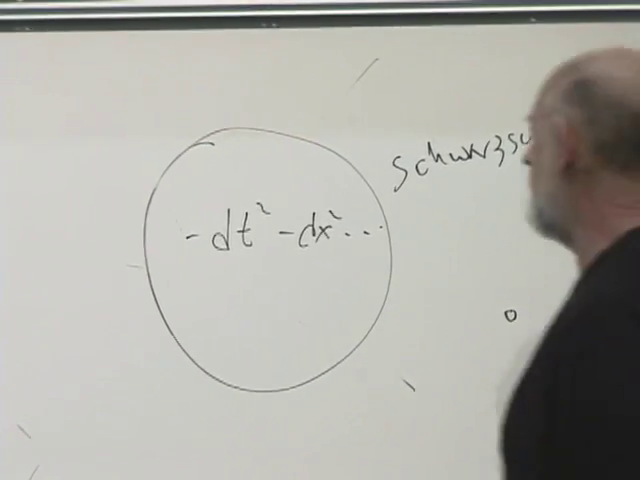
\includegraphics[width=0.74\textwidth]{lecture_04_figure_08.png}
\caption{球壳衔接图：圆内为平直时空，圆外为史瓦西解。}
\lectureframe{01:34:15.000}
\end{figure}

\begin{classroomqa}
\audiencequestion{在广义相对论中，球壳外部出现什么度规？\lecturetimestamp{01:33:17}}
\lecturerresponse{史瓦西度规，其质量参数等于球壳的总守恒质量。空的中心区域局部地是闵可夫斯基时空。}
\end{classroomqa}

\begin{classroomqa}
\audiencequestion{如果壳层收缩，为什么质量参数不改变？\lecturetimestamp{01:34:33}}
\lecturerresponse{因为总能量守恒。壳层的半径以及动能或束缚能贡献可能改变，但对于孤立球对称系统，守恒的外部质量是固定的。运动壳层改变的是平坦区域与施瓦西区域相连接的位置。}
\end{classroomqa}

内部平坦并不意味着内部时钟必然与无穷远处的时钟具有相同的归一化。跨壳层匹配可以将内部时间坐标乘以一个常数，而运动壳层需要相应的连接条件。\editorialnote{伯克霍夫定理在局部固定每个真空区域。它们坐标之间的整体关系由跨壳层匹配诱导度规和外曲率确定。这些细节被推迟，正如坍缩构造被推迟到下一讲一样。}

我们现在拥有形成所需的两个部分：收缩壳层内部的闵可夫斯基时空和其外部的施瓦西时空。当壳层向内运动时，它们的界面描绘出一个世界管。沿着该世界管穿过原本的施瓦西半径，将用规则的坍缩前区域取代图~\ref{fig:l04-eternal}中非物理的过去半部分，并揭示真实黑洞的事件视界从何处开始。

\chapter{构建黑洞与近视界之谜}

\lectureoverview{我们将用三块材料来构建一个黑洞：平直时空的因果图、施瓦西图，以及球壳的伯克霍夫定理。这一构建表明，事件视界是一个整体边界，并且可以起始于一个局部仍然平直的区域。随后我们从因果几何转向熵与霍金温度。置于视界附近的温度计会变得任意热，而自由下落的观测者却预期不会发生局部灾难。最后的论证追问：外部实验在不制造它本应探测的扰动的前提下，究竟能确立什么。}

\section{处于空空间温度下的黑洞}

本来应该有一份作业：构建一个黑洞并把它带到课堂上展示讲解。没有人有黑洞可以展示，但通过 Wolfram 找到的一个计算提供了一个更温和的开场问题。什么样的半径和质量会使一个黑洞的霍金温度接近宇宙微波背景的 \(3\,\mathrm{K}\) 温度？

\begin{classroomqa}
\audiencequestion{网站上计算了什么？\lecturetimestamp{00:00:39}}
\lecturerresponse{一个温度约为 \(3\,\mathrm{K}\) 的黑洞的半径。重点不在于精确计算，而在于对物理尺度的估计。}
\end{classroomqa}

这样的黑洞会暂时与其周围环境具有相同的温度，但这种平衡是不稳定的。施瓦西黑洞具有负热容。如果它变得比热浴稍热，它就会辐射，失去质量，并变得更热。如果它变得稍冷，它就会吸收，获得质量，并变得更冷。\editorialnote{这就是课堂上故意宽松的措辞背后精确的稳定性论证。正则热浴无法为孤立的施瓦西黑洞提供稳定的平衡。}

估计从 \(3\,\mathrm{K}\) 辐射的特征波长开始。

\begin{classroomqa}
\audiencequestion{约三开尔文的辐射对应什么波长？\lecturetimestamp{00:02:03}}
\lecturerresponse{教室里有人提出一厘米、\(21\) 厘米，甚至 \(10\) 米，最后才确定在微波波段。对于论证有用的数量级答案约为一厘米，小到足以开微波炉和面包盒的玩笑。}
\end{classroomqa}

典型的霍金量子的波长与施瓦西半径相当，相差数值因子：
\begin{equation}
\lambda_{\mathrm{H}}\sim R_s,
\qquad
R_s=\frac{2GM}{c^2}.
\label{eq:l05-scale}
\end{equation}
取课堂值 \(\lambda_{\mathrm H}\sim1\,\mathrm{cm}\) 得到 \(R_s\sim1\,\mathrm{cm}\)。由于一个太阳质量的黑洞半径只有几公里，而 \(R_s\) 正比于 \(M\)，相应的质量大致为
\begin{equation}
M\sim10^{-5}M_\odot,
\label{eq:l05-rough-mass}
\end{equation}
这属于行星尺度。这就是为什么讲座得出一个类似地球的估计。

\begin{classroomqa}
\audiencequestion{这与 Wolfram 的数值结果一致吗？\lecturetimestamp{00:05:53}}
\lecturerresponse{报告的结果更接近月球的质量。与粗略估计相比这听起来很小，但无论哪个答案都说明了预期的要点：这个物体不是能装进口袋的东西。}
\end{classroomqa}

保留常数可以解释这一差异。由
\begin{equation}
T_H=\frac{\hbar c}{4\pi k_B R_s},
\end{equation}
在 \(T_H=3\,\mathrm{K}\) 时可得，
\begin{equation}
R_s\simeq6.1\times10^{-5}\,\mathrm{m},
\qquad
M\simeq4.1\times10^{22}\,\mathrm{kg}.
\label{eq:l05-three-kelvin}
\end{equation}
这是月球而非地球的质量。微波波长、因子 \(4\pi\)，以及选择哪个黑体波长作为典型值，共同造成了快速估计与数值之间的差距。\editorialnote{方程~\eqref{eq:l05-three-kelvin}恢复了讲座在量纲估计中省略的数值因子。估计本身被保留，因为它是课堂上使用的路径。}

算术已经完成了它的使命。我们现在想要在数学上和想象中构建一个黑洞。完整的场方程对于当前目的来说太难了。图像将提供基本事实。

\section{第一个工作部件：平直时空}

使用以观测者为中心的极坐标并抑制角度。约化坐标为 \((t,r)\)，其中 \(r\geq0\)。这个约化图中的一个点不是四维时空中的一个点；除 \(r=0\) 外，它代表整个二维球面 \(S^2\)。

径向光线以 \(45^\circ\) 运动。入射光线到达原点，出射光线沿另一零方向离开原点。通过共形变换，无限半平面可以被压缩成有限的彭罗斯楔形。该变换不是唯一的。其本质性质是无穷远被带到有限边界，并且径向零方向保持在 \(45^\circ\)。用黑板上的话说，我们把图压扁了。

\begin{figure}[htbp]
\centering
\includegraphics[width=0.68\textwidth]{lecture_05_figure_02.png}
\caption{紧致化径向闵可夫斯基时空的上半部分。竖直边为\(r=0\)，而曲线族向紧致化无穷远处聚集。}
\lectureframe{00:11:41.560}
\end{figure}

\begin{figure}[htbp]
\centering
\begin{tikzpicture}[scale=0.94]
\coordinate (O) at (0,0);
\coordinate (P) at (0,3.8);
\coordinate (I) at (6.2,1.9);
\draw[very thick] (O)--(P)--(I)--cycle;
\foreach \y in {0.45,0.90,1.35,1.80,2.25,2.70,3.15} {
  \draw[gray!75] (0,\y) .. controls (2.0,\y-0.18) and (4.4,1.9) .. (I);
}
\draw[gray!75] (0.65,0.37) .. controls (1.55,1.20) and (1.55,2.60) .. (0.65,3.43);
\draw[gray!75] (1.30,0.74) .. controls (2.25,1.30) and (2.25,2.50) .. (1.30,3.06);
\draw[gray!75] (2.05,1.08) .. controls (3.00,1.46) and (3.00,2.34) .. (2.05,2.72);
\draw[gray!75] (3.00,1.36) .. controls (3.85,1.62) and (3.85,2.18) .. (3.00,2.44);
\node[left] at (0,1.9) {\(r=0\)};
\node[above] at (P) {\(i^+\)};
\node[right] at (I) {\(i^0\)};
\end{tikzpicture}
\caption{上半楔形区域的清晰版本。这些曲线是定性的等\(r\)线和等\(t\)线族，并非精确的坐标网格。}
\label{fig:l05-flat-wedge}
\end{figure}

固定\(r\)的世界线在紧致化前是竖直的，随后弯曲并在未来类时无穷远附近聚集。等\(t\)切片同样向空间无穷远聚集。这种聚集是坐标效应，而非物质的物理压缩。

\(45^\circ\)规则直接适用于径向光。具有角动量的光线可能不经过原点，而是到达一个非零的最近距离后向外返回。远离原点时，其投影运动看起来几乎是径向的；只有在最近距离附近，约化的\((t,r)\)轨迹才明显弯曲。至此，第一部分工作完成。

\section{第二部分工作：永恒施瓦茨席尔德}

最大延拓的施瓦茨席尔德解有两个外部菱形区域、一个未来黑洞区域和一个过去白洞区域。其上、下波浪形边界分别是未来奇点和过去奇点。对于由坍缩形成的黑洞，这一结构的大部分很快就会被丢弃，但普通的右侧外部区域正是我们所需的部分。

\begin{figure}[htbp]
\centering
\includegraphics[width=0.72\textwidth]{lecture_05_figure_03.png}
\caption{永恒施瓦茨席尔德图，右侧为普通外部区域及其示意性坐标网格。}
\lectureframe{00:16:55.975}
\end{figure}

\begin{figure}[htbp]
\centering
\begin{tikzpicture}[scale=0.88]
\coordinate (C) at (0,0);
\coordinate (TL) at (-2.0,2.0);
\coordinate (L) at (-4.0,0);
\coordinate (BL) at (-2.0,-2.0);
\coordinate (TR) at (2.0,2.0);
\coordinate (R) at (4.0,0);
\coordinate (BR) at (2.0,-2.0);
\draw[thick] (C)--(TL)--(L)--(BL)--(C);
\draw[thick] (C)--(TR)--(R)--(BR)--(C);
\draw[very thick,decorate,decoration={snake,amplitude=1.2pt,segment length=7pt}] (TL)--(TR);
\draw[very thick,decorate,decoration={snake,amplitude=1.2pt,segment length=7pt}] (BL)--(BR);
\draw[gray!75] (TR) .. controls (2.15,0.8) and (2.15,-0.8) .. (BR);
\draw[gray!75] (TR) .. controls (2.65,0.9) and (2.65,-0.9) .. (BR);
\draw[gray!75] (TR) .. controls (3.20,0.7) and (3.20,-0.7) .. (BR);
\draw[gray!75] (0.15,0.95) .. controls (1.5,0.82) and (2.9,0.40) .. (R);
\draw[gray!75] (0.10,0.35) .. controls (1.5,0.34) and (2.9,0.18) .. (R);
\draw[gray!75] (0.10,-0.35) .. controls (1.5,-0.34) and (2.9,-0.18) .. (R);
\fill (C) circle (1.6pt);
\node[above] at (TR) {\(i^+\)};
\node[below] at (BR) {\(i^-\)};
\node[right] at (R) {\(i^0,\ r=\infty\)};
\node[above] at (0,2.25) {\(r=0\), future singularity};
\node[below] at (0,-2.25) {\(r=0\), past singularity};
\node[rotate=45,above,font=\small] at (1.0,1.0) {\(r=2GM\)};
\node[font=\small] at (2.70,0.75) {\(r=6GM\)};
\node[font=\small] at (3.15,-0.75) {\(r=100GM\)};
\end{tikzpicture}
\caption{右侧外部区域在大半径处类似于平坦楔形。当\(c=1\)时，其内部零边为\(r=2GM\)；其他标注的半径是示意性示例。}
\label{fig:l05-eternal-schwarzschild}
\end{figure}

远离黑洞处，外部区域越来越像紧致化的平坦空间。诸如\(r=6GM\)和\(r=100GM\)这样的线趋近于普通等半径世界线的行为。外部区域的内边界位于
\begin{equation}
r=2GM
\end{equation}
单位为\(c=1\)。

在中心附近，与平坦空间的比较失效。闵可夫斯基空间中的径向光线到达\(r=0\)后从相反的物理侧重新出现。施瓦茨席尔德内部指向未来的光线不会反弹。它终止于\(r=0\)处的类空奇点。这一因果差异正是坍缩构造必须保持的。

\section{让我们把各部分拼接起来的定理}

缺失的要素首先出现在牛顿引力中。对于球对称质量分布，高斯定律给出
\begin{equation}
\oint\mathbf g\cdot d\mathbf A=-4\pi G M_{\mathrm{enc}},
\end{equation}
因此
\begin{equation}
\mathbf g(r)=-\frac{G M_{\mathrm{enc}}(r)}{r^2}\,\hat{\mathbf r}.
\label{eq:l05-shell-theorem}
\end{equation}
半径\(r\)的球面之外的物质对该处不贡献净场。对于总质量为\(M\)的空心球壳，
\begin{equation}
\mathbf g=
\begin{cases}
0, & r<R_{\mathrm{shell}},\\[3pt]
-\dfrac{GM}{r^2}\hat{\mathbf r}, & r>R_{\mathrm{shell}}.
\end{cases}
\end{equation}

伯克霍夫定理是相对论性的替代。每个球对称真空区域局部上都是具有恒定质量参数的施瓦茨席尔德区域。球形壳层的空内部质量参数为零，局部上是闵可夫斯基的；外部质量参数为\(M\)，是施瓦茨席尔德的：
\begin{equation}
\begin{aligned}
M_{\mathrm{enc}}&=0 && \text{inside the shell},\\
M_{\mathrm{enc}}&=M && \text{outside the shell}.
\end{aligned}
\label{eq:l05-birkhoff}
\end{equation}
当壳层运动时，该陈述仍然有用，因为两侧的真空区域保持球对称。

\editorialnote{内部平坦是一个局部陈述。即使内部曲率消失，静态壳层也可以改变内部时间坐标的归一化。对于运动或零壳层，两个真空度规必须在壳层处匹配；理想化构造是薄壳连接，与入射Vaidya几何密切相关。这些限定条件都不改变此处使用的因果剪贴论证。}

对于实验室图像，想象一个球面密布着同步激光器，如同大型惯性约束装置中那样，全部同时向内发射。在理想化中不存在仪器，只有一个完美球形的光壳层。壳层携带能量\(E\)，因此外部质量参数为
\begin{equation}
M=\frac{E}{c^2},
\end{equation}
或在自然单位下简写为\(E=M\)。由于壳层以光速运动，它在约化图上是一条入射零线。该线上的每个点代表整个球面波前，而非单个光子轨迹。

\section{缝合坍缩时空}

从平坦时空开始，画出入射零壳层。壳层内部是正确的：伯克霍夫定理表明它是平坦的。壳层外部是错误的，因为外部必须已经通过其施瓦茨席尔德几何知道壳层的总质量。

现在在永恒施瓦茨席尔德图中画出同一个壳层。在那里，壳层外部的区域是正确的。对于从普通真空中开始的坍缩而言，白洞、第二个外部区域以及黑洞内部不适当的部分都是错误的，因此把它们擦掉。

\begin{figure}[htbp]
\centering
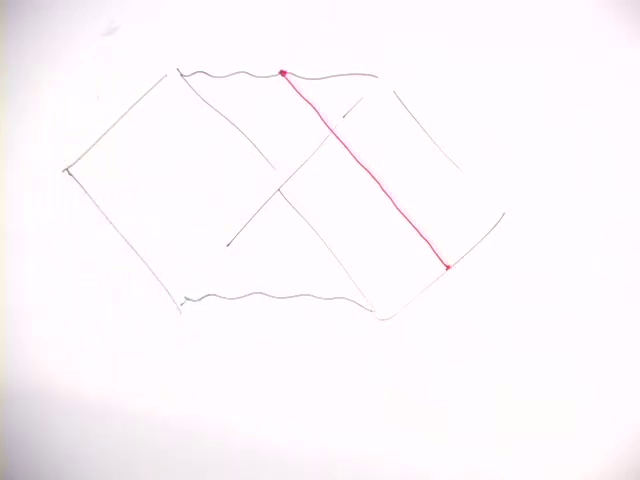
\includegraphics[width=0.72\textwidth]{lecture_05_figure_05.png}
\caption{零质量壳层，以红色表示，画在施瓦茨席尔德图上，同时正确的部分被分离出来。}
\lectureframe{00:32:00.000}
\end{figure}

壳层在平坦部分到达\(r=0\)。在施瓦茨席尔德部分，它到达未来奇点的起点。这两个是同一个端点。沿壳层把平坦内部与施瓦茨席尔德外部粘合起来，就得到黑洞形成的最简单时空。

\begin{classroomqa}
\audiencequestion{在左上方的连接点处，平坦空间的端点真的与施瓦茨席尔德一侧的点相同吗？\lecturetimestamp{00:34:50}}
\lecturerresponse{是的。平坦空间中的壳层收缩到\(r=0\)，而施瓦茨席尔德奇点也在\(r=0\)。被等同起来的这两个点具有相同的几何意义：二维球面已经收缩到零尺度。}
\end{classroomqa}

\begin{figure}[htbp]
\centering
\begin{tikzpicture}[scale=0.96]
\coordinate (A) at (0,-2.8);
\coordinate (B) at (0,1.65);
\coordinate (C) at (2.05,1.65);
\coordinate (D) at (5.4,-0.15);
\coordinate (E) at (3.75,3.10);
\coordinate (H0) at (0,-0.45);
\draw[very thick] (A)--(B);
\draw[very thick] (A)--(D)--(E);
\draw[very thick,red!75!black] (D)--(B);
\draw[very thick,decorate,decoration={snake,amplitude=1.2pt,segment length=7pt}] (B)--(C);
\draw[very thick,green!45!black] (H0)--(C);
\draw[thick] (C)--(E);
\node[left] at (0,0.45) {\(r=0\)};
\node[below right] at (3.95,-0.05) {ingoing null shell};
\node[font=\small] at (1.25,-1.35) {flat interior};
\node[font=\small,anchor=west] at (2.55,2.38) {Schwarzschild exterior};
\node[above,font=\small] at (1.0,2.02) {\(r=0\) singularity};
\node[above left,font=\small] at (0.98,0.62) {event horizon};
\node[right] at (E) {\(i^+\)};
\end{tikzpicture}
\caption{坍缩几何。红色壳层把平坦内部与施瓦茨席尔德外部连接起来。绿色事件视界在平坦区域中开始得更早，并终止于黑洞区域的未来边界。}
\label{fig:l05-collapse}
\end{figure}

这一构造回答了永恒解所遗留的一个问题。由坍缩形成的黑洞没有过去的白洞，也没有第二个渐近宇宙。它仍然有一个未来奇点。

\section{视界是一个整体边界}

旧的标签\(r=2GM\)在静态施瓦茨席尔德几何中标识了视界，但它并不是动力学时空中所需的定义。

\begin{definition}
未来事件视界是能够向未来零无穷发送未来指向因果信号的事件集合的边界。
\end{definition}

在坍缩图上，追踪那条恰好无法逃逸的向外零射线。紧靠它外侧的射线到达无穷远；紧靠它内侧的射线终止于奇点。那个分隔者就是真正的视界。

\begin{figure}[htbp]
\centering
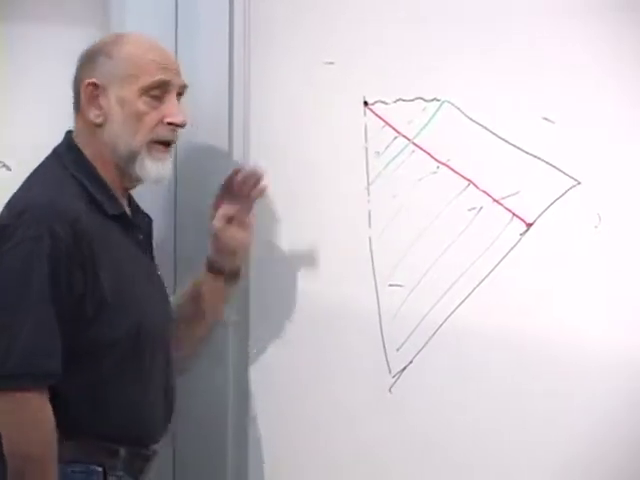
\includegraphics[width=0.72\textwidth]{lecture_05_figure_06.png}
\caption{完成的黑板构造。入射壳层为红色，事件视界为绿色；绿线的一部分位于壳层下方仍为平坦的区域中。}
\lectureframe{00:39:10.000}
\end{figure}

令人惊讶的特征现在不可避免。视界向后延伸到壳层尚未到达的区域。那里的几何局部是平坦的，穿过那条线的观测者不会探测到曲率脉冲、墙或闪光。然而，该观测者已经无法到达无穷远，因为未来的壳层将封闭所有可能的逃逸路径。事件视界正是在这种整体意义上具有目的论性质：定位一个事件视界需要知道时空的整个未来。\editorialnote{没有任何局部实验能够确定一个光滑的事件视界刚刚被穿过。其他概念，例如表观视界或捕获视界，更为局部，并且在坍缩过程中不必与事件视界重合。}

排水口类比隔离出了因果观念。想象一个划船者位于静止湖中一个被塞住的排水口附近。如果塞子永远不拔，划船者可以离开。如果某人必定会拔掉它，那么即使水尚未流动，后来的水流也可能使逃逸变得不可能。冻结的尼亚加拉瀑布说明了同一点：平静的水并不保证未来有通往安全的路线。

\begin{classroomqa}
\audiencequestion{塞子被拔掉是因为光的球面壳层变得越来越集中吗？\lecturetimestamp{00:43:13}}
\lecturerresponse{这种集中创造了黑洞，但排水口故事被用于一个更狭窄的目的：在局部发生任何戏剧性事件之前，一个人可能已经越过了不可返回点。}
\end{classroomqa}

\subsection{由增长球面构成的视界}

约化视界上的每一点都代表一个\(S^2\)。在视界的第一个点处，该球面面积为零。沿视界向上移动，球面不断增长，直到其面积半径达到
\begin{equation}
R_s=\frac{2GM}{c^2}.
\end{equation}
对于静态黑洞，它保持该尺度；如果有更多能量落入，它会再次增长。

\editorialnote{在理想化球对称坍缩图中，视界生成元在\(r=0\)上的一个形成点或折痕处相交。正是这个极限二维球面具有零面积；不应把该陈述理解为有限的施瓦茨席尔德视界突然收缩到一个点。}

\subsection{遥远观测者能够重构什么}

接下来的长篇讨论把已经处于整体视界内部的观测者与该观测者如何到达那里的历史区分开来。

\begin{classroomqa}
\audiencequestion{在壳层到达之前，被困者的状态是什么？从远处观察者的角度来看，那个人是否在视界之外？\lecturetimestamp{00:44:03}}
\lecturerresponse{不。一旦世界线位于事件视界之后，它的未来就到达奇点，并且它发出的任何新信号都无法到达远处观察者。然而，那个人并非在那里开始存在。更早的粒子、祖先或其他前驱能量是从一个可见区域进入的。}
\end{classroomqa}

因此，远处观察者可能看到前驱物质接近视界，却从未接收到来自视界之外的信号。看穿入射壳层并无矛盾：它由光构成，观察者也能看到壳层本身，并推断黑洞已经形成。

\begin{classroomqa}
\audiencequestion{视线是否穿过坍缩壳层，外部观察者是否仍能知道黑洞已经形成？\lecturetimestamp{00:46:51}}
\lecturerresponse{是的。观察者看到入射壳层，并且能够接收到其路径穿过该壳层的光，只要那光仍能逃逸。看起来奇怪的是，前驱物质甚至在壳层到达中心之前就接近了新确定的视界。}
\end{classroomqa}

\begin{classroomqa}
\audiencequestion{这是否延续了那条规则：从外部看，物质看起来像是被压缩到了视界上？\lecturetimestamp{00:47:49}}
\lecturerresponse{是的。在外部描述中，它仍然与视界相关联，红移越来越大，直到后来黑洞蒸发的量子过程改变了这一图景。}
\end{classroomqa}

这种外部描述引出了下一个主题。如果信息看起来被涂抹在一个二维表面上，那么黑洞熵与该表面面积成正比就不那么令人惊讶了。

\section{从无穷远处看到的熵与温度}

在大视界附近，我们可以用局部平面代替球面，就像在小实验室中使用平地近似一样。于是，先前讨论中的两个事实被结合起来：
\begin{equation}
\begin{aligned}
S_{\mathrm{BH}}&\propto A_H,\\
\Delta A_H&\sim \ell_P^2
\quad\text{per added bit, schematically}.
\end{aligned}
\end{equation}
每普朗克面积一个比特的助记法表达了面积律；它不是微观推导。

在远离施瓦茨席尔德黑洞处测得的霍金温度为
\begin{equation}
T_H=\frac{\hbar c^3}{8\pi GMk_B}.
\label{eq:l05-hawking}
\end{equation}
以\(R_s=2GM/c^2\)代入，
\begin{equation}
T_H=\frac{\hbar c}{4\pi k_B R_s}.
\label{eq:l05-hawking-radius}
\end{equation}
因此较大的黑洞更冷。

\begin{classroomqa}
\audiencequestion{温度可以依赖于位置吗？\lecturetimestamp{00:52:43}}
\lecturerresponse{在日常交谈中，它显然可以：纽约和斯坦福不必具有相同的温度。更精确的问题涉及处于引力热平衡的系统。在那里，尽管红移后的平衡温度是常数，局部温度计读数仍可随高度变化。}
\end{classroomqa}

温度是通过局部动能来读取的。在被加热的地球上方的稀薄大气中，分子上升时失去动能，下降时获得动能。光子向上红移，向下蓝移。因此，低处温度计和高处温度计不必记录相同的局部能量标度。

对于静态时空，平衡关系为
\begin{equation}
T_{\mathrm{loc}}(r)\sqrt{-g_{tt}(r)}=T_\infty,
\label{eq:l05-tolman}
\end{equation}
即托尔曼定律。方程~\eqref{eq:l05-hawking}中的霍金温度为\(T_\infty\)，即在无穷远处归一化的读数。

\section{视界附近的热静态大气}

设\(\rho\)为从视界向外的固有距离。在大施瓦茨席尔德视界附近，方程~\eqref{eq:l05-tolman}变为
\begin{equation}
k_B T_{\mathrm{loc}}(\rho)
\simeq\frac{\hbar c}{2\pi\rho},
\label{eq:l05-local-temperature-si}
\end{equation}
或者，在以\(c=\hbar=k_B=1\)为单位时，
\begin{equation}
T_{\mathrm{loc}}(\rho)=\frac{1}{2\pi\rho}.
\label{eq:l05-local-temperature}
\end{equation}

\begin{figure}[htbp]
\centering
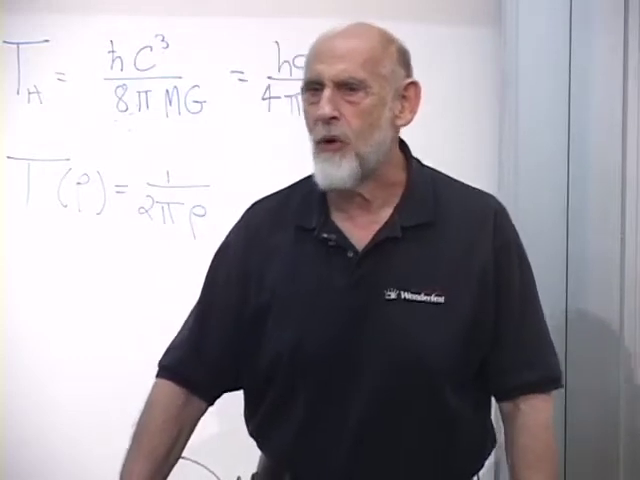
\includegraphics[width=0.72\textwidth]{lecture_05_figure_07.png}
\caption{渐近霍金温度与黑板上的视界附近局部温度\(T(\rho)=1/(2\pi\rho)\)。}
\lectureframe{01:02:40.000}
\end{figure}

一个用缆绳固定在\(\rho\)处的微小温度计，在被放下时会报告温度升高。维持在该静态大气中的原子会先被激发，然后电离，再解离；在更大的局部能量下，甚至原子核和强子也无法保持完整。让人脚朝下下降会得到令人难忘的诊断：热脚。

\emph{保持}一词至关重要。这种发散属于由加速保持静止的探测器。它描述的是相对于外部时间红移的热大气。自由下落的探测器遵循不同的轨迹，并且对于处于正则量子态中的足够大的黑洞，不必在视界处遇到发散的浴场。\editorialnote{这一区分将静态观察者看到的托尔曼温度和加速温度与自由下落观察者的正则局部体验区分开来。讲座有意将这种对比变成一个操作性问题，而不是仅靠术语来解决它。}

电离阈值使这一冲突变得具体。

\begin{classroomqa}
\audiencequestion{电离氢需要多少能量？\lecturetimestamp{01:06:53}}
\lecturerresponse{课堂上给出的是\(13\)电子伏特，正确地指出了\(13.6\,\mathrm{eV}\)基态电离能。随附的几千开尔文的估计太小，但论证只需要存在一个有限的阈值。}
\end{classroomqa}

确实，
\begin{equation}
\frac{13.6\,\mathrm{eV}}{k_B}\simeq1.58\times10^5\,\mathrm{K}.
\end{equation}
因此存在某个小的固有距离\(\rho_{\mathrm{ion}}\)，在该处静态温度达到电离尺度。静态外推表明，原子在那里——在视界之外——就应该已经电离了。相比之下，自由下落的原子预期不存在局域的墙，并且可以在有限的固有时间内穿过视界。外部观察者能否进行一项实验，在这两种描述之间做出判定？

\section{海森堡显微镜}

在把这个问题应用于黑洞之前，先回顾一下光子显微镜。要以分辨率\(\Delta x\)定位一个粒子，探测波长必须满足
\begin{equation}
\lambda\lesssim\Delta x.
\end{equation}
此时一个光子至少携带动量
\begin{equation}
p_\gamma\gtrsim\frac{\hbar}{\Delta x}.
\label{eq:l05-microscope}
\end{equation}
散射该光子会产生同量级的反冲。如果先测量位置，随即检查速度，那么第二次测量所看到的是已被第一次测量改变的状态。这个实验制造出了它本意要排除的条件。

\begin{figure}[htbp]
\centering
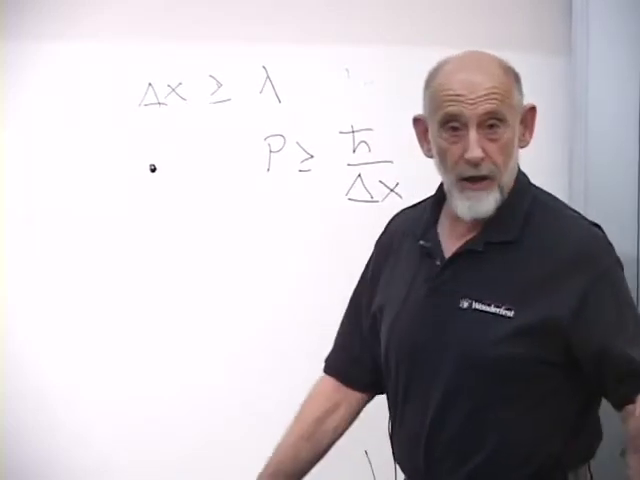
\includegraphics[width=0.70\textwidth]{lecture_05_figure_08.png}
\caption{显微镜估计\(\Delta x\gtrsim\lambda\)和\(p_\gamma\gtrsim\hbar/\Delta x\)。}
\lectureframe{01:11:50.000}
\end{figure}

这不仅仅是经典光学的局限。经典波可以被弄得任意弱；而量子力学要求在一次成功的探测事件中至少有一个量子。因此，提高空间分辨率就迫使产生有限的动量转移。

\section{近视界实验}

现在让一个原子从\(\rho_{\mathrm{ion}}\)处开始穿过这一层。相对于静态参考系，它以接近\(c\)的速度向内运动，因此在穿过视界之前可用的时间间隔为
\begin{equation}
\Delta\tau\sim\frac{\rho_{\mathrm{ion}}}{c}.
\label{eq:l05-fall-time}
\end{equation}
穿过之后，任何结果都无法传回外部。测量必须在这段短暂的时间间隔内区分完好的原子与电离的原子。

要在该层内分辨原子，需要
\begin{equation}
\lambda\lesssim\rho_{\mathrm{ion}}.
\end{equation}
因此探测能量受限于
\begin{equation}
E_\gamma=cp_\gamma
\gtrsim\frac{\hbar c}{\rho_{\mathrm{ion}}}.
\label{eq:l05-probe-energy}
\end{equation}
除因子\(2\pi\)外，这与方程~\eqref{eq:l05-local-temperature-si}是同一尺度：
\begin{equation}
E_\gamma\gtrsim2\pi k_B T_{\mathrm{loc}}(\rho_{\mathrm{ion}}).
\label{eq:l05-probe-temperature}
\end{equation}
能量足以分辨该事件的光子，其能量也足以电离该原子。

\begin{figure}[htbp]
\centering
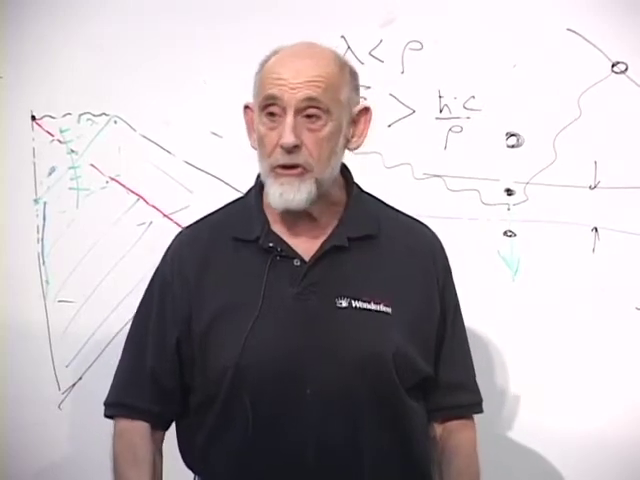
\includegraphics[width=0.72\textwidth]{lecture_05_figure_09.png}
\caption{黑板上的近视界估计：\(\lambda<\rho\)迫使局域探测能量达到\(\hbar c/\rho\)量级。}
\lectureframe{01:18:30.000}
\end{figure}

\begin{classroomqa}
\audiencequestion{那个高能光子在原子自身的自由下落参考系中也会电离该原子吗？\lecturetimestamp{01:19:07}}
\lecturerresponse{会。原子被一个真实的能量量子击中，并在其自身的局域参考系中反冲或电离。测量所揭示的并不是不受干扰的下落；它用受扰的下落取代了不受扰的下落。}
\end{classroomqa}

\begin{classroomqa}
\audiencequestion{如果原子只是下落，而没有人进行这个实验呢？\lecturetimestamp{01:19:39}}
\lecturerresponse{那么这种特定的扰动就不存在。如果外部观察者确实进行了高分辨率实验，原子就有麻烦了。这个论证关心的是从外部能够验证什么，而不是证明一个未被测量的下落者会被烧毁。}
\end{classroomqa}

\subsection{温度计或发射器能做得更好吗？}

移动仪器并不能消除信息问题。

\begin{classroomqa}
\audiencequestion{能否在更远处测量、推断梯度，或者让一个自由下落的温度计记录温度并在以后取回？\lecturetimestamp{01:19:51}}
\lecturerresponse{要获知近视界的记录，必须有某物与温度计相互作用，并以量子的形式把信息送回来。让温度计掉头需要剧烈的加速，而远程读取它则需要发射或散射。无论哪条途径，都会改变那个本应被检验其未受扰历史的物理系统。}
\end{classroomqa}

\begin{classroomqa}
\audiencequestion{小分辨率所需的高探测能量，与把反射观测从近视界区域送出去，是同一个困难吗？\lecturetimestamp{01:21:51}}
\lecturerresponse{它们是同一个红移尺度的两面。光子在最终到达无穷远时可以能量很低，因为它爬出来时损失了能量，但在它分辨原子的地方，它必须具有很高的局域频率。}
\end{classroomqa}

\editorialnote{仅仅为了逃逸，在视界外侧不远处发射的光子并不需要具有很大的能量。这里决定性的要求是，它要在\(\rho\)量级的固有时间和距离内编码该事件；于是引力红移把那个很大的局域频率与一个小得多的渐近频率联系起来。}

\begin{classroomqa}
\audiencequestion{物体能否自己发出信息，而不是被外部光子击中？\lecturetimestamp{01:22:51}}
\lecturerresponse{可以，但局域发射仍然需要足够的带宽，以辨认在短促时间间隔内发生了什么。发射还会给物体带来反冲。用发射器取代反射光，并不会产生无需代价的记录。}
\end{classroomqa}

\begin{classroomqa}
\audiencequestion{下落的原子有一个优先方向。它那有方向的动能被称为温度吗？\lecturetimestamp{01:23:10}}
\lecturerresponse{不是。扔出一个棒球并不会使棒球变热。整体下落能量与热骚动是不同的。论证中的温度属于周围静态辐射大气，而不属于原子的质心运动。}
\end{classroomqa}

\begin{classroomqa}
\audiencequestion{共同下落的实验室能否用磁场来检验原子是否被电离？\lecturetimestamp{01:23:50}}
\lecturerresponse{实验室可以进行局域检验。困难在于在穿越之前把结果传回外部。这种通信同样需要相互作用以及具有必要局域分辨率的出射量子。}
\end{classroomqa}

\begin{classroomqa}
\audiencequestion{如果温度计内置发射器，它会不会需要如此多的局域能量，以致摧毁仪器？\lecturetimestamp{01:24:57}}
\lecturerresponse{这就是同一障碍的工程形式。在足够靠近视界处，相关局域尺度上所需的信号能量与被检验的热尺度相当。}
\end{classroomqa}

\begin{classroomqa}
\audiencequestion{高温区域是否薄得没有时间从容进行测量？\lecturetimestamp{01:25:15}}
\lecturerresponse{正是如此。其固有厚度为\(\rho\)量级，穿越时间为\(\rho/c\)量级。人们可以把这一限制描述为空间分辨率或时间带宽；无论哪种描述，都要求高的局域动量或能量。}
\end{classroomqa}

相应的时间-带宽估计为
\begin{equation}
\Delta E\,\Delta\tau\gtrsim\hbar.
\end{equation}
这里应把它读作傅里叶分辨率或操作分辨率界限，而不是读作与\(\Delta x\,\Delta p\geq\hbar/2\)地位相同的算符不确定性关系。讲座只是启发式地援引时间-能量不确定性；由空间分辨率导出的方程~\eqref{eq:l05-probe-energy}才是论证中更坚实的部分。

\begin{classroomqa}
\audiencequestion{能否对许多原子使用较低能量、较低分辨率的探针，并以统计方式恢复答案？\lecturetimestamp{01:26:26}}
\lecturerresponse{这是一个合理的问题，课堂上对此保持开放。每个原子只提供一次通过，而任何被恢复的信号仍必须携带足够信息，以辨认短促的近视界事件。讲座诉诸不确定性原理，但并未给出完整的统计不可行性证明。}
\end{classroomqa}

\enlargethispage{2\baselineskip}
\section{已经确立与尚未确立的内容}

该论证并不预言自由下落者必定感受到发散的静态温度。

\begin{classroomqa}
\audiencequestion{我们是在说，我们可以预言下落者不会感受到温度吗？\lecturetimestamp{01:27:38}}
\lecturerresponse{不是。结论更狭窄：一个旨在确认原子未经历高温扰动的外部实验，会造成同一尺度的扰动。这就是这一操作分析所确立的全部内容。}
\end{classroomqa}

因此，结论不是防火墙定理，也不是下落者被烧毁的证明，更不是什么都不会发生的证明。它是对外部验证的限制：\emph{分辨未受扰动的近视界事件，需要一个会扰动它的探针}。
如果进行该实验，其量子就会产生它本要检验的效应。如果不进行该实验，仅凭这一论证并不能指定任何额外的实验上可及的事实。与双缝实验的类比是有意为之：在没有路径测量的情况下追问走了哪条缝，以及在没有相互作用的情况下追问外部装置能证实什么，都是在所提议的证据无法获得之处试图附加一个操作答案。

\chapter{长弦与黑洞对应}

\lectureoverview{黑洞具有熵，因此它必定拥有微观自由度。我们将建立关于这些自由度的最简单的弦论描述：首先对一条长激发弦的态进行计数，然后改变弦耦合，直到弦的描述与黑洞的描述相遇。最后的等式被有意留作下一讲要完成的问题。}

\section{熵要求微观载体}

说一个系统具有很大的熵，就是说它能够隐藏大量的微观信息。一浴缸热水可能具有量级为\(10^{30}\)的熵。这一陈述已经告诉我们，存在着数量极其巨大的微观自由度，无论我们是否选择逐个分子地去检视它们。热力学可以通过测量能量和温度来确定熵，但它并不指认携带熵的对象。

流体动力学使这一区分变得熟悉。它描述密度、速度、压强和宏观流动，而不提及原子。加上热力学，人们就会发现流体具有熵。熵宣告了一种粗粒化方程并不显示的微观结构；它引出一个新问题，而不是回答它。

黑洞以更尖锐的形式提出了同样的挑战。Bekenstein的提议，经Hawking的计算而完成，赋予熵一个与视界面积成正比的量。广义相对论确定了几何及其热力学，但它没有给出微观态的清单。那些其组态解释了面积律的微小而众多的对象是什么？在弦理论中存在一个具体的候选者。这里展开的论证是有意定性的：它把参数依赖关系弄对了，同时略去了数值常数和完整态计数的形式化机器。

\section{三个尺度与一个记号上的危险}

引力提供了一个特殊的长度，即普朗克长度，
\begin{equation}
\ell_p=\sqrt{\frac{G_N\hbar}{c^3}}.
\label{eq:l06-planck-si}
\end{equation}

\begin{classroomqa}
\audiencequestion{\(G_N\)、\(\hbar\)和\(c\)的哪种组合给出普朗克长度？\lecturetimestamp{00:06:08}}
\lecturerresponse{是\(\sqrt{G_N\hbar/c^3}\)，约为\(10^{-33}\)厘米。我们将立即令\(\hbar=c=1\)，于是该关系变得简单得多。}
\end{classroomqa}

在自然单位下，
\begin{equation}
\hbar=c=1,
\qquad
G_N=\ell_p^2.
\label{eq:l06-planck-area}
\end{equation}
因此牛顿常数具有面积的量纲。这就是为什么一个面积除以\(G_N\)是无量纲的，并且可以是一个熵。

弦理论有第二个长度，\(\ell_s\)。加热一条弦，或把它置于高度激发的态，它就会在许多尺度上摆动。在这一基本图像中，特征性的最短尺度是弦长。人们可以把\(\ell_s\)视为与弦振荡的一个基本单元相关联的尺度。

第三个量是无量纲的弦耦合\(g_s\)。它控制分裂与合并：一条弦可以掐断成两条弦，或者一条激发弦可以发射一个闭弦量子。

\begin{classroomqa}
\audiencequestion{弦耦合的物理意义是什么？\lecturetimestamp{00:09:20}}
\lecturerresponse{它控制弦发生相互作用的几率，例如当一条弦与自身相交时的分裂。更确切地说，\(g_s\)是相互作用振幅；相应的概率或速率从\(g_s^2\)阶开始。}
\end{classroomqa}

所发射的无质量闭弦激发可以是一个引力子。在这方面，\(g_s\)扮演着类似于电荷的角色：它是附着在一个相互作用顶点上的因子。\editorialnote{本讲在把\(g_s\)称为概率和称为振幅之间交替。在微扰论中，它是振幅层面的耦合；概率和速率则包含它的平方。}

\section{为什么引力知道\texorpdfstring{\(g_s^2\)}{耦合的平方}}

首先考虑电磁学的交换图像。一个带电物体发射一个光子，带有一个\(e\)因子，第二个物体吸收它，又带有一个\(e\)因子。因此交换振幅包含\(e^2\)。这一图像并不是字面意义上的经典抛射物故事，但它正确地显示了耦合如何进入。

\begin{figure}[htbp]
\centering
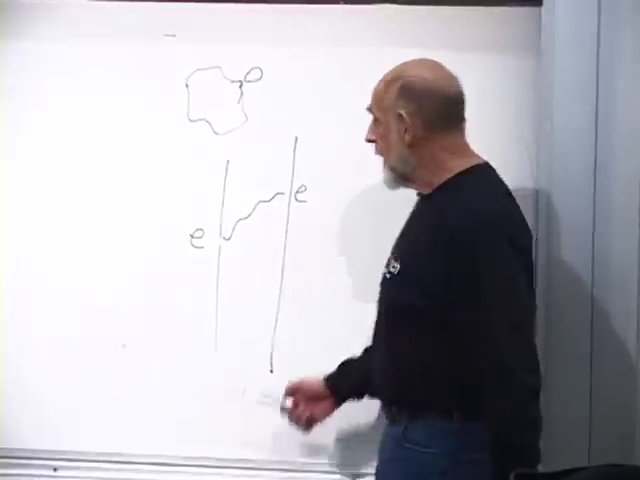
\includegraphics[width=0.72\textwidth]{lecture_06_figure_03.png}
\caption{黑板上完成的交换草图：一个耦合附着在发射处，又附着在吸收处。}
\lectureframe{00:11:30.000}
\end{figure}

弦理论的版本把光子替换为引力子，把电荷替换为\(g_s\)。一个因子伴随发射，另一个伴随吸收，因此引力强度按\(g_s^2\)标度。

在长距离下，同一相互作用必须重现牛顿的力定律，
\begin{equation}
F_{\mathrm{grav}}\sim G_N\frac{M_1M_2}{r^2}.
\end{equation}
质量和平方反比依赖关系描述源和传播；这里所需的要点是乘在它们前面的耦合。

\begin{figure}[htbp]
\centering
\begin{tikzpicture}[x=1cm,y=1cm]
  \node[font=\small\bfseries] at (1.8,3.55) {electromagnetism};
  \draw[line width=0.8pt] (0,0) -- (0,3);
  \draw[line width=0.8pt] (3.6,0) -- (3.6,3);
  \draw[line width=0.8pt] plot[smooth] coordinates {(0,1.5) (0.45,1.72) (0.9,1.28) (1.35,1.72) (1.8,1.28) (2.25,1.72) (2.7,1.28) (3.15,1.72) (3.6,1.5)};
  \node[below] at (0,1.42) {\(e\)};
  \node[below] at (3.6,1.42) {\(e\)};
  \node[font=\small] at (1.8,0.25) {exchange strength \(\propto e^2\)};
  \node[font=\small\bfseries] at (7.2,3.55) {string gravity};
  \draw[line width=0.8pt,rounded corners=6pt] (5.4,0) -- (5.2,0.7) -- (5.5,1.5) -- (5.25,2.3) -- (5.4,3);
  \draw[line width=0.8pt,rounded corners=6pt] (9,0) -- (9.2,0.7) -- (8.9,1.5) -- (9.15,2.3) -- (9,3);
  \draw[line width=0.8pt] plot[smooth] coordinates {(5.5,1.5) (5.95,1.72) (6.4,1.28) (6.85,1.72) (7.3,1.28) (7.75,1.72) (8.2,1.28) (8.65,1.72) (8.9,1.5)};
  \node[below] at (5.5,1.42) {\(g_s\)};
  \node[below] at (8.9,1.42) {\(g_s\)};
  \node[font=\small] at (7.2,0.25) {exchange strength \(\propto g_s^2\)};
\end{tikzpicture}
\caption{耦合计数类比。交换的量子每一端贡献一个相互作用因子。}
\end{figure}

这一观察几乎确定了牛顿常数。耦合\(g_s\)是无量纲的，而在四维中\(G_N\)具有长度的平方的量纲。可用的微观长度是\(\ell_s\)，因此
\begin{equation}
G_N\sim g_s^2\ell_s^2.
\label{eq:l06-newton-string}
\end{equation}
将其与方程~\eqref{eq:l06-planck-area}结合，得到
\begin{equation}
\ell_p\sim g_s\ell_s.
\label{eq:l06-planck-string}
\end{equation}

\begin{figure}[htbp]
\centering
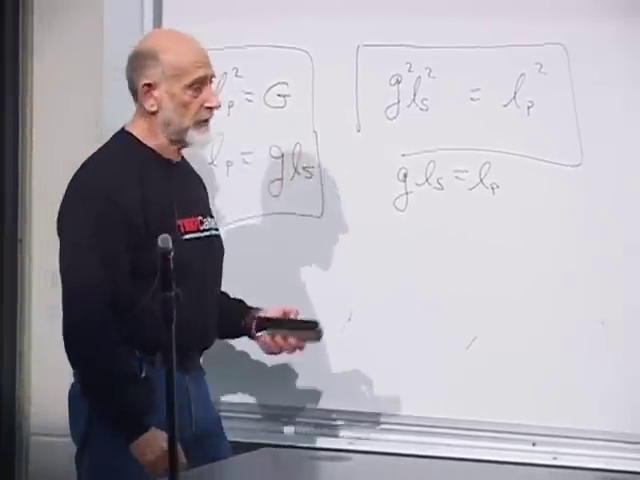
\includegraphics[width=0.72\textwidth]{lecture_06_figure_04.png}
\caption{黑板上保留的基本关系：\(\ell_p^2=G_N\)和\(\ell_p\sim g_s\ell_s\)。}
\lectureframe{00:15:45.000}
\end{figure}

方程~\eqref{eq:l06-newton-string}是本讲中始终使用的简化关系。\editorialnote{在紧致化的弦理论中，有效四维牛顿常数还依赖于紧致化体积和量级为一的约定。本讲将这些数据略去，以分离出对应关系的标度行为。}

\begin{classroomqa}
\audiencequestion{\(g_s\)大于还是小于一，哪个长度更大？\lecturetimestamp{00:16:00}}
\lecturerresponse{我们在弱耦合下工作，\(g_s<1\)。于是\(\ell_p\sim g_s\ell_s\)意味着弦长大于普朗克长度。强耦合需要不同的描述，此处不需要。}
\end{classroomqa}

\section{黑洞计数}

略去玻尔兹曼常数和数值因子，贝肯斯坦--霍金熵为
\begin{equation}
S_{\mathrm{BH}}=\frac{A}{4G_N}sim\frac{A}{G_N}sim\frac{A}{\ell_p^2}.
\label{eq:l06-bh-area}
\end{equation}
因子\(1/4\)在半经典公式中是精确的，但在这一标度论证中不起作用。

\begin{classroomqa}
\audiencequestion{下标``BH''是指黑洞还是贝肯斯坦--霍金？\lecturetimestamp{00:16:51}}
\lecturerresponse{就我们的目的而言，它可以同时提醒我们两者。重要的陈述是：熵是以普朗克面积度量的视界面积。}
\end{classroomqa}

对于四维施瓦茨席尔德黑洞，
\begin{equation}
R_s=2G_NM,
\qquad
A=4\pi R_s^2.
\end{equation}
如本讲所做的那样略去\(2\)和\(4\pi\)，
\begin{align}
S_{\mathrm{BH}}
&\sim \frac{R_s^2}{G_N}
\sim \frac{(G_NM)^2}{G_N} \\
&\sim M^2G_N
\sim M^2\ell_p^2.
\label{eq:l06-bh-mass}
\end{align}
这就是我们将与弦计数相比较的形式。

\section{长弦作为随机游走}

从一根小弦开始，向其中注入能量。一般的高激发弦不会保持为整齐的圈。它变成一个长而缠结的物体，就像卷线器严重缠乱后的钓鱼线。这一缠结具有熵，因为大量构型在宏观上看起来相同。

为了对它们计数，将空间替换为链路长度为\(\ell_s\)的点阵。格点是顶点，链路是线，基本方格是面。弦由连通的链路序列表示。这个模型是刻意粗糙的，但其指数式的态计数捕捉到了所需的标度行为。

\begin{figure}[htbp]
\centering
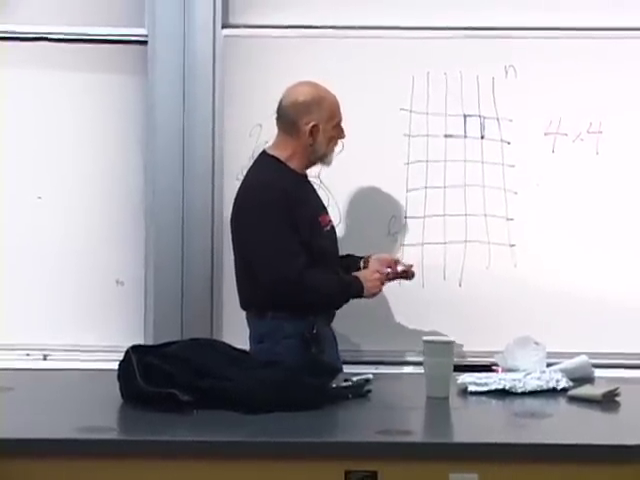
\includegraphics[width=0.72\textwidth]{lecture_06_figure_05.png}
\caption{二维点阵模型。蓝色线段标记弦的一步；在每个格点处对四种可能的延续进行计数。}
\lectureframe{00:23:50.000}
\end{figure}

\begin{classroomqa}
\audiencequestion{在这个玩具游走的每一步有多少种选择？\lecturetimestamp{00:22:43}}
\lecturerresponse{在正方点阵上是四种，因为允许立即回退。在三维中会有六种。换一种点阵会改变这个普通数字，但不会改变游走数目随链路数指数增长这一事实。}
\end{classroomqa}

如果弦有\(n\)条链路，二维玩具计数为
\begin{equation}
\Omega_n\sim4^n.
\label{eq:l06-walk-count}
\end{equation}
存在一种例外的直线游走，但它只是\(4^n\)中的一个态。典型的游走反复折叠，占据一个缠结的球。对于大的\(n\)，几乎每一个随机生成的构型在定性上都与任何其他构型相同。

熵是宏观上不可区分构型数目的对数：
\begin{equation}
S_{\mathrm{st}}=\log\Omega_n\sim n\log4\sim n.
\label{eq:l06-string-entropy-n}
\end{equation}

\begin{classroomqa}
\audiencequestion{为什么熵变得正比于\(n\)而不是\(4^n\)？\lecturetimestamp{00:25:39}}
\lecturerresponse{熵是态数目的对数。因此\(\log(4^n)=n\log4\)，而因子\(\log4\)是量级为一的常数，我们将把它略去。}
\end{classroomqa}

如果\(L\)是从弦的一端沿弦到另一端所得到的轮廓长度，那么
\begin{equation}
n=\frac{L}{\ell_s},
\qquad
S_{\mathrm{st}}\sim\frac{L}{\ell_s}.
\label{eq:l06-string-entropy-length}
\end{equation}
这里\(L\)不是缠结球的直径。它是沿弦测量的长得多的距离。

接下来我们用轮廓长度换取质量。在\(c=\hbar=1\)下，质量具有长度的倒数的量纲。因此一条弦尺度大小的链路携带量级为
\begin{equation}
m_{\mathrm{link}}\sim\frac{1}{\ell_s}.
\label{eq:l06-link-mass}
\end{equation}的质量

\begin{classroomqa}
\audiencequestion{为什么一条链路的质量必须按\(1/\ell_s\)标度？\lecturetimestamp{00:29:20}}
\lecturerresponse{在这些单位下，质量是长度的倒数，而\(\ell_s\)是唯一可用的长度。等价地，量级为\(1/\ell_s^2\)的弦张力乘以链路长度\(\ell_s\)给出相同的结果。}
\end{classroomqa}

于是完整弦具有
\begin{equation}
M\sim n m_{\mathrm{link}}
\sim\frac{n}{\ell_s}
\sim\frac{L}{\ell_s^2},
\qquad
L\sim M\ell_s^2.
\label{eq:l06-string-mass}
\end{equation}
将其代入方程~\eqref{eq:l06-string-entropy-length}得到
\begin{equation}
S_{\mathrm{st}}\sim M\ell_s.
\label{eq:l06-string-entropy-mass}
\end{equation}
点阵行走忽略了世界面约束和数值系数，但高度激发弦谱的指数增长给出了相同的领头标度行为。\editorialnote{随机行走构造是弦态高能级密度的一个助记手段，而不是对基本弦的字面离散化。}

\section{引发论证的不匹配}

现在两个答案为
\begin{equation}
S_{\mathrm{BH}}\sim M^2\ell_p^2,
\qquad
S_{\mathrm{st}}\sim M\ell_s.
\label{eq:l06-two-entropies}
\end{equation}
它们彼此相似，但在固定质量和任意耦合下并不相等。黑洞表达式对\(M\)是二次的；弦表达式则是线性的。不能简单地宣称热弦就是黑洞，而不解释这两个区域如何衔接。

\begin{figure}[htbp]
\centering
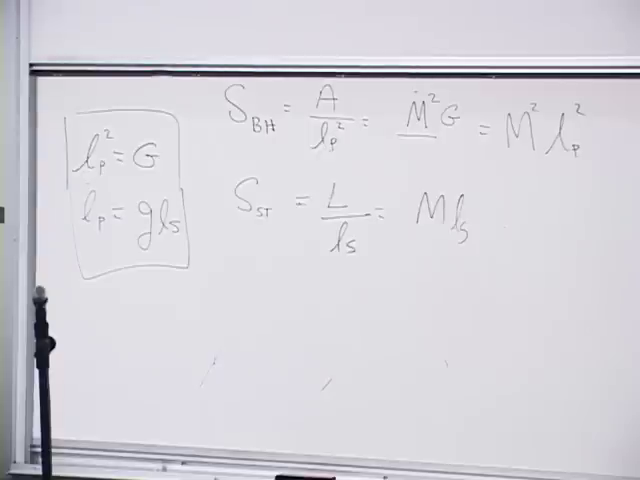
\includegraphics[width=0.78\textwidth]{lecture_06_figure_06.png}
\caption{无遮挡的板书对比：上方为黑洞熵，下方为长弦熵，左侧保留普朗克--弦关系。}
\lectureframe{00:33:20.000}
\end{figure}

课堂正是在这里暂停了。这种悬念是有用的：不匹配并非这一思想的失败，而是提示我们必须比较同一个态，同时改变引力的强度。

\section{转动耦合旋钮}

保持\(\ell_s\)固定，设想\(g_s\)可以变化。在\(g_s=0\)处，弦既不分裂也不结合，引力消失，因为\(G_N\sim g_s^2\ell_s^2\)。此时一个能量足够高的态就是一根长而弱相互作用的弦。

缓慢增大\(g_s\)。弦相互作用成为可能，而更重要的是，就当前论证而言，引力增强了。

\begin{classroomqa}
\audiencequestion{随着\(g_s\)增大，第一个效应是否仅仅是弦分裂成更短的弦？\lecturetimestamp{00:36:29}}
\lecturerresponse{分裂与结合成为可能，但保持\(\ell_s\)固定并追踪高熵态。核心效应是\(G_N\)增大，因此长弦的自引力将纠缠的球向内拉。}
\end{classroomqa}

该物体收缩并变得更致密。其引力势能为负，因此收缩降低其总能量，从而降低其质量。

\begin{classroomqa}
\audiencequestion{当自引力将弦拉在一起时，能量是增加还是减少？\lecturetimestamp{00:37:48}}
\lecturerresponse{它减少。结合能变得更负。尽管我们继续追踪同一个态，沿路径的质量不必保持不变。}
\end{classroomqa}

最终该物体的尺度与其施瓦西半径相当。超过这一点，黑洞描述就是自然的描述。更大的初始激发在更小的耦合下达到这一条件，因为更 massive 的物体形成视界所需的引力强度更小。

\begin{figure}[htbp]
\centering
\resizebox{0.95\linewidth}{!}{%
\begin{tikzpicture}[x=1cm,y=1cm,>=Latex]
  \draw[->,line width=0.9pt] (0,0) -- (11,0) node[right] {increasing \(g_s\)};
  \node[draw,rounded corners,align=center,minimum width=2.6cm,minimum height=1.15cm] at (1.8,1.5) {long excited string\\weak self-gravity};
  \node[draw,rounded corners,align=center,minimum width=2.6cm,minimum height=1.15cm] at (5.5,1.5) {correspondence point\\\(R_s\sim\ell_s\)};
  \node[draw,circle,align=center,minimum size=1.8cm] at (9.3,1.5) {black\\hole};
  \draw[->,line width=0.8pt] (3.15,1.5) -- (4.1,1.5) node[midway,above,font=\small] {contracts};
  \draw[->,line width=0.8pt] (6.9,1.5) -- (8.25,1.5);
  \node[font=\small,align=center] at (5.5,-0.65) {same family of states followed slowly;\\binding energy and mass may change};
\end{tikzpicture}
}
\caption{固定\(\ell_s\)下的对应路径。反转箭头将黑洞态带回长弦态。}
\end{figure}

\begin{classroomqa}
\audiencequestion{我们是否应设想\(g_s\)介于零和一之间？\lecturetimestamp{00:40:18}}
\lecturerresponse{是的。论证仍处于弱耦合区域。如果\(g_s\)非常小，则该态必须相应地非常 massive 才能成为黑洞。我们不需要进入控制很差的\(g_s>1\)区域。}
\end{classroomqa}

在思想实验中，缓慢的变化是可逆的。

\begin{classroomqa}
\audiencequestion{如果我们把耦合调回去，直到引力不再能把黑洞束缚在一起，它会变成什么？\lecturetimestamp{00:41:37}}
\lecturerresponse{一根长弦。在引力消失时，这一构造中的一切都必须用弦态来描述。朝一个方向转动旋钮将弦映射为黑洞；转回来则将黑洞映射为弦。}
\end{classroomqa}

在固定总能量和固定体积内，占主导的高熵构型本质上是一根长弦，而不是数量巨大的短弦。这一陈述在此并未推导。它是弦在Hagedorn区域附近的统计力学结果，之后会重新讨论。

\section{外部观察者看到什么}

当该物体被描述为黑洞时，弦在哪里？在外部描述中，它并不会突然消失。施瓦西时间将表观穿越送到任意晚的时间，因此弦的自由度被表示为在视界上或视界附近积累。

\begin{figure}[htbp]
\centering
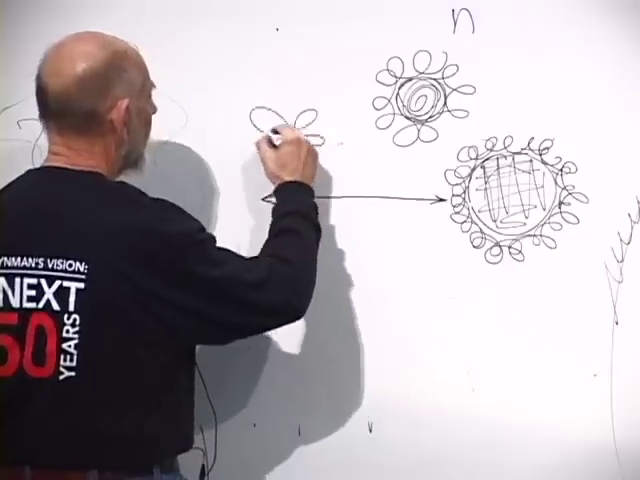
\includegraphics[width=0.72\textwidth]{lecture_06_figure_07.png}
\caption{板书对比：宏观视界中弦尺度结构只是薄薄的绒毛，而较小视界的半径接近圈尺度。}
\lectureframe{00:45:30.000}
\end{figure}

对于\(R_s\gg\ell_s\)，黑洞是宏观的，弦尺度结构相对于视界半径而言只是一层薄薄的壳层。当半径减小到接近\(\ell_s\)时，光滑黑洞与延展弦之间的区分就失去了意义。这是一种外部的、拉伸视界描述；不应将其与一种坐标无关的断言相混淆，即下落物质永远不会穿过一个规则视界。\editorialnote{讲座使用的是黑洞互补性中为人熟知的外部描述。短语``在视界上''指的是由外部描述所分辨的自由度，而不是对其协变位置的独立推导。}

交叉发生在
\begin{equation}
R_s\sim\ell_s.
\label{eq:l06-correspondence-radius}
\end{equation}
低于弦尺度时，施瓦茨席尔德几何无法分辨本应支撑它的结构。圈从本应是视界的位置涨落开去，该态更适合被称为弦。

\section{对应点}

在方程~\eqref{eq:l06-correspondence-radius}中使用\(R_s\sim G_NM\)：
\begin{equation}
G_NM\sim\ell_s.
\end{equation}
然后代入\(G_N\sim g_s^2\ell_s^2\)：
\begin{equation}
M g_s^2\ell_s^2\sim\ell_s,
\qquad
M g_s^2\ell_s\sim1.
\label{eq:l06-correspondence-condition}
\end{equation}

\begin{figure}[htbp]
\centering
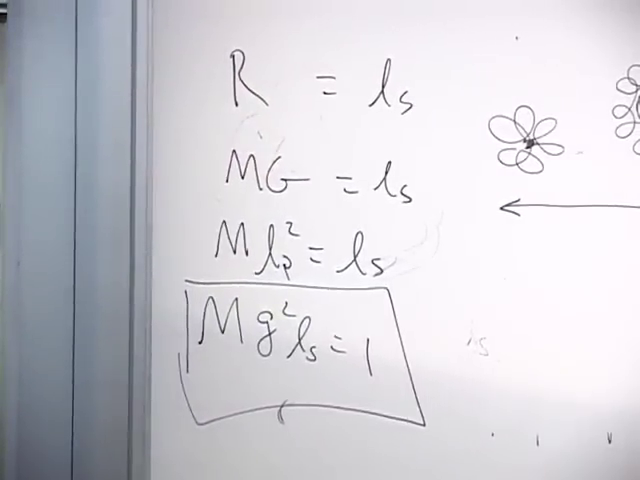
\includegraphics[width=0.72\textwidth]{lecture_06_figure_08.png}
\caption{黑板上完成的过渡代数：\(R_s\sim\ell_s\)导致加框的无量纲条件\(Mg_s^2\ell_s\sim1\)。}
\lectureframe{00:49:50.000}
\end{figure}

一位听众注意到了这个条件正在准备什么。在对应点，
\begin{align}
S_{\mathrm{BH}}
&\sim M^2\ell_p^2
\sim M^2g_s^2\ell_s^2 \\
&=(M\ell_s)(Mg_s^2\ell_s)
\sim M\ell_s
\sim S_{\mathrm{st}}.
\label{eq:l06-entropy-preview}
\end{align}

\begin{classroomqa}
\audiencequestion{这些方程是否已经意味着黑洞熵与弦熵变得相等？\lecturetimestamp{00:50:18}}
\lecturerresponse{是的。这正是计算所要达到的地方。各个要素已经放在黑板上，但讲座推迟了它们的完整组装，以便能够仔细审视对应的逻辑。}
\end{classroomqa}

方程~\eqref{eq:l06-entropy-preview}是这次交流中隐含的一行代数预览。它确立了标度关系，而不是精确系数\(1/4\)。精确的微观匹配需要更受控的黑洞和更详细的弦构造。\editorialnote{讲座在将方程~\eqref{eq:l06-entropy-preview}作为其完整推导呈现之前就停止了。这里将其写出，是因为听众明确指出了这一等式，而且所有所需的关系都已经出现过。}

\section{为什么熵可以被携带过去}

还剩下一个逻辑要素。假设一个控制参数，例如磁场或\(g_s\)，在系统孤立且演化可逆的情况下被足够缓慢地改变。能量、大小和结合能可能改变，但熵保持不变：
\begin{equation}
\Delta S=0.
\label{eq:l06-adiabatic-entropy}
\end{equation}
讲座将此与信息守恒联系起来。熵衡量的是被粗粒化描述所隐藏的信息；哈密顿量的缓慢可逆变化重新排列了态，而没有删除该信息。

\begin{classroomqa}
\audiencequestion{熵恒定是否要求路径避开相变？\lecturetimestamp{00:54:01}}
\lecturerresponse{是的，必须能够连续地跟踪该态。有限系统没有无限体积那种严格非解析的热力学相变，而且如果变化足够缓慢，对应可以被视为光滑的交叉。}
\end{classroomqa}

这里使用的绝热是更强的准静态、可逆意义。绝热但不可逆的过程可以产生熵；缓慢性和跟踪态的能力是必不可少的。\editorialnote{热力学陈述\(\Delta S=0\)要求一条可逆绝热路径。在量子力学中，相应的想法是当参数变化时跟踪同一组态，而不发生不受控的能级跃迁。}

\begin{classroomqa}
\audiencequestion{为什么一根长弦会比携带相同总质量的几根较短弦具有更多熵？\lecturetimestamp{00:54:44}}
\lecturerresponse{这反直觉，但显式的高能态计数在固定体积中偏向长弦成分。证明被推迟；就目前的论证而言，我们只需要黑洞映射到最大熵的弦部门，而不是映射到由极多短弦组成的稀薄气体。}
\end{classroomqa}

因此操作策略是：
\begin{enumerate}
\item 从耦合\(g_{s,0}\)下质量为\(M_0\)的黑洞开始。
\item 缓慢降低\(g_s\)，同时跟踪同一高熵态族。
\item 停在\(R_s\sim\ell_s\)处，此时黑洞描述变为长弦描述。
\item 使用\(S_{\mathrm{st}}\sim M\ell_s\)计数弦态。
\item 将该熵沿可逆路径带回原来的黑洞。
\end{enumerate}

\begin{figure}[htbp]
\centering
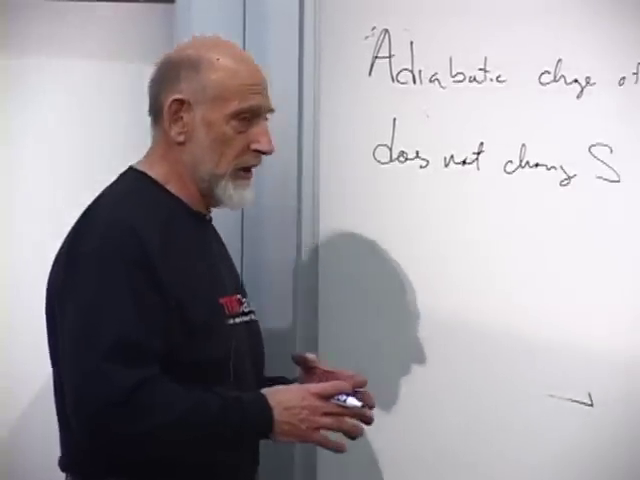
\includegraphics[width=0.72\textwidth]{lecture_06_figure_09.png}
\caption{在陈述策略时保留在黑板上的一条原理：\(g_s\)的绝热变化不改变\(S\)。}
\lectureframe{00:56:40.000}
\end{figure}

弦理论已经为带电、旋转、超对称、近极端以及高维黑洞给出了更为精确的熵计数。这里关于中性Schwarzschild黑洞的讨论是粗略的对应论证：它确定了态密度的参数依赖关系和物理交叉，而不是精确的受保护简并度。\editorialnote{精确一致对于态计数在耦合变化时受到保护的特殊黑洞最为有力。本讲有意给出最简单的量级版本。}

\begin{classroomqa}
\audiencequestion{当引力被关闭时，态是否可能变成两根弦，而不是恰好一根？\lecturetimestamp{00:58:25}}
\lecturerresponse{存在有限概率出现少量长弦，而使用两根而非一根不会改变主导的熵标度。会改变论证的是碎裂成大量短弦组成的气体；高能统计计数并不支持这一结果。}
\end{classroomqa}

黑洞是能够装入一个区域的最大熵，而长弦是引力被移除时相应的高熵态。这两种描述现在已被联系起来，但尚未发展成精确计算。下一步是仔细重复代数运算，并追问这一对应关系可以被信任到何种程度。

\chapter{黑洞熵、全息性与德西特空间}

\lectureoverview{我们完成上一讲开始的那个对应关系论证。高度激发的弦具有正比于其质量的熵，而施瓦茨席尔德黑洞具有正比于其面积的熵。这两个公式之间的联系，并不是通过把一个强引力黑洞等同于一条自由弦而建立的，而是通过缓慢改变弦耦合，直到两种描述相遇。面积定律于是自然地导向全息原理，而本讲的最后一部分引入膨胀空间以及德西特几何，其视界将在下一讲研究。}

\section{回到计数问题}

长弦计数中还有一个未了结之处。如果把一个固定的总长度分配给若干条弦，那么长度相同的全同弦是不可区分的。然而它们在盒子中的位置仍然是态的一部分，而盒子的尺寸被选为大致等于相应的单条长弦所占据的大小。

\begin{classroomqa}
\audiencequestion{这些短弦彼此可区分吗，它们的位置要计入吗？\lecturetimestamp{00:00:37}}
\lecturerresponse{性质全同的弦是不可区分的，但它们在盒子中的位置要计入。比较是在固定体积下进行的，该体积被选为与长弦所占据的区域相匹配。}
\end{classroomqa}

这一点确定之后，我们就可以陈述目标了。我们将汇集一个简短的方程清单，并用它们得到黑洞熵的标度关系。不需要积分或无穷求和。困难不在于代数；困难在于知道哪些量可以比较，以及在论证的哪个阶段进行比较。

\section{自然单位与普朗克面积}

令
\begin{equation}
c=\hbar=1,
\label{eq:l07-natural-units}
\end{equation}
但保持牛顿常数显式出现。第一个推论是时间和长度具有相同的单位。光子关系式
\begin{equation}
E=\frac{\hbar c}{\lambda}
\end{equation}
以及质能关系 \(E=mc^2\) 于是给出
\begin{equation}
[M]=L^{-1}.
\label{eq:l07-mass-dimension}
\end{equation}
因此质量可以表示为长度的倒数。

\begin{figure}[htbp]
\centering
\includegraphics[width=0.62\textwidth]{lecture_07_figure_02.png}
\caption{量纲论证开始时采用的自然单位约定。能量公式已在上面的方程中补全。}
\lectureframe{00:03:27.900}
\end{figure}

要确定 \(G_N\) 的单位，只需把牛顿加速度用作量纲记账：
\begin{equation}
a\sim\frac{G_NM}{R^2}.
\end{equation}
因为 \(T\) 和 \(L\) 具有相同的单位，所以 \([a]=L/T^2=L^{-1}\)。结合方程~\eqref{eq:l07-mass-dimension}，这给出
\begin{equation}
[G_N]=L^2.
\end{equation}
在这些单位下，牛顿常数是一个面积。通过
\begin{equation}
G_N=\ell_p^2,
\label{eq:l07-planck-area}
\end{equation}
定义普朗克长度，我们立刻明白为什么 \(A/G_N=A/\ell_p^2\) 是无量纲的：它度量的是以普朗克面积计的面积。

\section{弦耦合与引力的强度}

现在必须把引力翻译成弦的语言。有用的图像是交换过程。当一条弦与自身相交时，它可以分裂并重新连接。一个小闭弦圈可以由一个物体发射并被另一个物体吸收；当该激发是引力子时，这个过程就传递引力。发射时出现一个相互作用因子，吸收时又出现一个，因此交换强度中含有 \(g_s^2\)。

耦合 \(g_s\) 是无量纲的。更准确地说，它是振幅层面的耦合，而概率或速率从 \(g_s^2\) 阶开始。\editorialnote{本讲有时把 \(g_s\) 称为概率，随后又更正为概率的平方根。微扰耦合属于振幅层面。} 由于 \(G_N\) 具有面积的量纲，仍然缺少一个长度标度。基本弦长 \(\ell_s\)，即一次基本弦振动的尺度，提供了它：
\begin{equation}
G_N\sim g_s^2\ell_s^2,
\qquad
\ell_p\sim g_s\ell_s.
\label{eq:l07-planck-string}
\end{equation}

\begin{figure}[htbp]
\centering
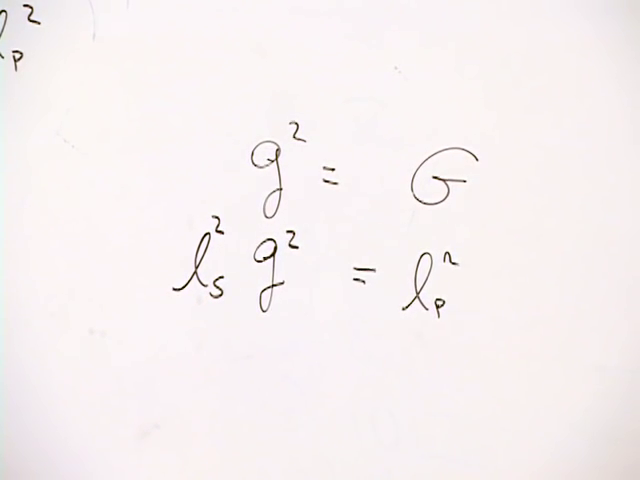
\includegraphics[width=0.72\textwidth]{lecture_07_figure_05.png}
\caption{黑板上的耦合关系：\(G_N=\ell_p^2\) 和 \(g_s^2\ell_s^2\sim\ell_p^2\)。}
\lectureframe{00:12:15.000}
\end{figure}

在弱耦合下，\(g_s\ll1\)，普朗克长度远小于弦长。把 \(g_s\) 调小会削弱引力，同时使基本弦标度保持不变。\editorialnote{对于有效的四维理论，紧致化数据和数值约定也会进入 \(G_N\)。它们被保持固定，并在这个标度论证中被略去。}

\section{计数一条长弦}

熵计数的是指定一个态所需的基本决定。把一条高度激发的弦替换为在正方形点阵上的行走。在每个顶点，下一段连线可以指向四个方向之一。无论这个基本选择被描述为一次四向决定还是两次二元决定，改变的只是一个量级为一的常数。重要的是步数。

如果\(L\)是弦的轮廓长度，而每一步的长度为\(\ell_s\)，那么需要
\begin{equation}
N=\frac{L}{\ell_s}
\end{equation}
步。行走的数目呈指数增长，示意性地为\(\Omega_N\sim q^N\)，其中\(q\)为1阶量，因此
\begin{equation}
S_{\mathrm{str}}=\log\Omega_N\sim N\sim\frac{L}{\ell_s}.
\label{eq:l07-string-entropy-length}
\end{equation}

\begin{figure}[htbp]
\centering
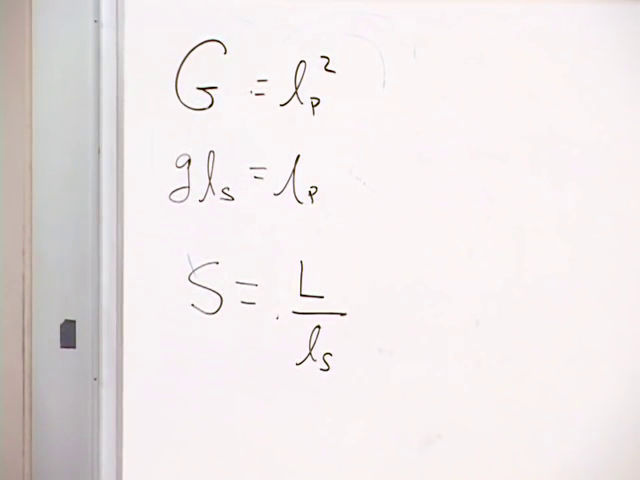
\includegraphics[width=0.68\textwidth]{lecture_07_figure_03.png}

\vspace{0.7em}
\begin{tikzpicture}[scale=0.82]
  \draw[step=0.8cm,gray!45,thin] (0,0) grid (6.4,4.0);
  \draw[very thick,blue!60!black]
    (0.8,0.8)--(1.6,0.8)--(1.6,1.6)--(2.4,1.6)--(2.4,2.4)--
    (3.2,2.4)--(3.2,1.6)--(4.0,1.6)--(4.0,2.4)--(4.8,2.4)--
    (4.8,3.2)--(5.6,3.2);
  \draw[<->,thick] (0.8,-0.35)--(1.6,-0.35);
  \node[below] at (1.2,-0.35) {step \(\ell_s\)};
  \node[align=center] at (8.1,2.0) {\(N=L/\ell_s\) steps\\[0.3em]\(S_{\mathrm{str}}\sim N\)};
\end{tikzpicture}
\caption{黑板上的点阵模型及其整理后的随机行走解释。决定选择数目的是轮廓长度，而不是缠结球的直径。}
\lectureframe{00:17:20.000}
\end{figure}

质量由同样的基本线段来计数。长度为\(\ell_s\)的线段具有质量标度
\begin{equation}
m_{\mathrm{seg}}\sim\frac{1}{\ell_s}.
\end{equation}

\begin{classroomqa}
\audiencequestion{基本线段被赋予长度\(\ell_s\)吗？\lecturetimestamp{00:18:56}}
\lecturerresponse{是的。它的特征长度为\(\ell_s\)，因此在自然单位下其特征质量为\(1/\ell_s\)。}
\end{classroomqa}

将\(L/\ell_s\)个线段的质量相加得到
\begin{equation}
M\sim\frac{L}{\ell_s}\frac{1}{\ell_s}
=\frac{L}{\ell_s^2},
\qquad
L\sim M\ell_s^2.
\label{eq:l07-string-mass}
\end{equation}
振荡弦的动能和势能已被压缩进这个标度关系；详细的统计力学处理给出相同的依赖关系。代入方程~\eqref{eq:l07-string-entropy-length}便得到我们所需的弦公式：
\begin{equation}
S_{\mathrm{str}}\sim M\ell_s.
\label{eq:l07-string-entropy-mass}
\end{equation}

\begin{figure}[htbp]
\centering
\includegraphics[width=0.66\textwidth]{lecture_07_figure_04.png}
\caption{比较之前所汇总的弦一侧各列：\(\ell_p\sim g_s\ell_s\)、\(S_{\mathrm{str}}\sim L/\ell_s\sim M\ell_s\)和\(M\sim L/\ell_s^2\)。}
\lectureframe{00:21:57.800}
\end{figure}

\section{为什么自由弦还不是黑洞}

在引力一侧，精确的半经典公式为
\begin{equation}
S_{\mathrm{BH}}=\frac{A}{4G_N}.
\label{eq:l07-bh-exact}
\end{equation}

\begin{classroomqa}
\audiencequestion{分母中应取什么数值系数？\lecturetimestamp{00:23:28}}
\lecturerresponse{4。对应论证将恢复标度关系，但过于粗糙，无法确定那个精确因子。}
\end{classroomqa}

对于四维施瓦茨席尔德黑洞，
\begin{equation}
R_s=2G_NM,
\qquad
A=4\pi R_s^2.
\end{equation}
如讲座所做的那样略去数值常数，
\begin{align}
S_{\mathrm{BH}}
&\sim\frac{A}{G_N}
\sim\frac{(G_NM)^2}{G_N} \\
&\sim M^2G_N
\sim M^2\ell_p^2.
\label{eq:l07-bh-scaling}
\end{align}

\begin{figure}[htbp]
\centering
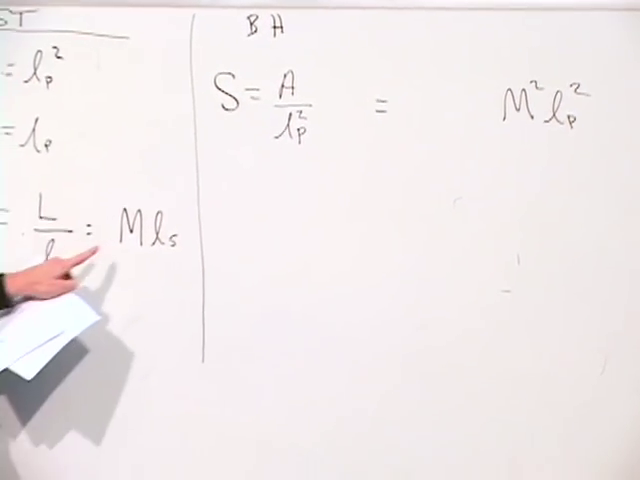
\includegraphics[width=0.72\textwidth]{lecture_07_figure_06.png}
\caption{黑板上完成的比较：弦熵是以弦单位为单位的长度，而黑洞熵是以普朗克单位为单位的面积。}
\lectureframe{00:25:35.000}
\end{figure}

方程~\eqref{eq:l07-string-entropy-mass}与\eqref{eq:l07-bh-scaling}之间的相似性具有启发性，但它们并非同一个公式。简单地把原来的黑洞称为自由弦并代入，是错误的。自由弦计数忽略了弦各部分之间的吸引相互作用，而正是这种相互作用把弦压缩成黑洞，并通过负结合能降低其总能量。

恒星使这一错误变得熟悉。把恒星质量的热气体放入一个过大的盒子中，并不是恒星的模型，即使温度相同。自引力会改变平衡尺寸以及能量与熵之间的关系。追踪长弦的每一个自相互作用会很困难，因此我们将避免这样做。

\begin{classroomqa}
\audiencequestion{如果一个小环从长弦上离开，它的熵会减少。那么引力子交换是否因此降低引力系统的熵？\lecturetimestamp{00:28:48}}
\lecturerresponse{在此处所使用的平衡交换过程中并非如此。虚激发沿两个方向发射和吸收；这幅漫画并不是永久失去一个弦片段的字面过程。它目前唯一的目的是确定两个耦合因子，从而确定\(g_s^2\)依赖关系。}
\end{classroomqa}

\section{绝热对应游戏}

不如从引力可忽略之处开始。当\(g_s\to0\)时，弦相互交叉而不分裂或合并，自引力吸引消失。增大\(g_s\)，同时保持\(\ell_s\)固定：引力增强，高度激发的弦收缩，最终变成黑洞。缓慢反向转动旋钮，黑洞必须回到弦态。它可能变成少量长弦，但上一讲的高能计数表明，主导扇区包含一根长弦，而不是由大量短弦组成的气体。

\begin{classroomqa}
\audiencequestion{改变耦合时保持什么固定？\lecturetimestamp{00:32:19}}
\lecturerresponse{弦长\(\ell_s\)，因而基本弦质量标度\(1/\ell_s\)，保持固定。旋钮改变\(g_s\)，从而改变\(G_N\sim g_s^2\ell_s^2\)。}
\end{classroomqa}

变化必须是缓慢、孤立且可逆的。在这些条件下，熵是绝热不变量：
\begin{equation}
\Delta S=0.
\label{eq:l07-adiabatic}
\end{equation}
如果发生耗散或不受控的跃迁，仅靠缓慢是不够的。这里``绝热''意味着同一族态可以被连续追踪。\editorialnote{这是绝热一词的可逆热力学含义。不可逆过程可以在无热流的意义上是绝热的，却仍然产生熵。}

设目标黑洞的质量为 \(M_0\)，耦合为 \(g_{s,0}\)。在使用我们试图解释的面积公式之前，量纲分析只能说明：一个中性、不旋转黑洞的熵是如下无量纲组合的某个函数
\begin{equation}
S_{\mathrm{BH}}=f(M\ell_p)
=f(Mg_s\ell_s).
\label{eq:l07-entropy-function}
\end{equation}
在 \(\ell_s\) 固定时，一条等熵路径因此保持
\begin{equation}
Mg_s=M_0g_{s,0}
\label{eq:l07-adiabat}
\end{equation}
不变，前提是沿着同一支态进行。

随着 \(g_s\) 减小，负结合能被移除，因此质量 \(M\) 沿此路径上升。底层的弦构型也变得更松散并延展开来。然而，形式上的施瓦茨席尔德半径在绝热线上表现为 \(R_s\sim Mg_s^2\ell_s^2\sim g_s\ell_s\)，因此反而减小。\editorialnote{口头讨论中用 ``增长'' 来描述从引力束缚中释放出来的物体。不应将其理解为施瓦茨席尔德半径沿所导出的绝热线增长。}

\begin{classroomqa}
\audiencequestion{当引力被减弱时，该物体是增长还是收缩？\lecturetimestamp{00:36:28}}
\lecturerresponse{它的弦结构被释放并膨胀，而它的质量增加，因为负结合能被移除。由黑洞公式给出的半径减小，直到达到弦尺度，在那里这种黑洞描述不再有用。}
\end{classroomqa}

\section{两条曲线及其交点}

纵轴为质量，横轴为弦耦合。方程~\eqref{eq:l07-adiabat} 是一条双曲线，\(M\propto g_s^{-1}\)。

\begin{classroomqa}
\audiencequestion{乘积 \(Mg_s\) 为常数的曲线是什么类型？\lecturetimestamp{00:44:08}}
\lecturerresponse{一条双曲线。它是通过目标点 \((g_{s,0},M_0)\) 的绝热线。}
\end{classroomqa}

第二条曲线标志着两种描述之间的过渡。一旦黑洞的半径小于基本弦的涨落尺度，它就不能被分辨为传统的施瓦茨席尔德几何。因此我们通过下式估计对应点
\begin{equation}
R_s\sim\ell_s.
\label{eq:l07-correspondence-radius}
\end{equation}
利用 \(R_s\sim MG_N\) 和方程~\eqref{eq:l07-planck-string}，这变为
\begin{equation}
Mg_s^2\ell_s^2\sim\ell_s,
\qquad
Mg_s^2\sim\frac{1}{\ell_s}.
\label{eq:l07-transition-curve}
\end{equation}
因此过渡曲线按 \(M\propto g_s^{-2}\) 下降，比绝热线更陡。

\begin{figure}[htbp]
\centering
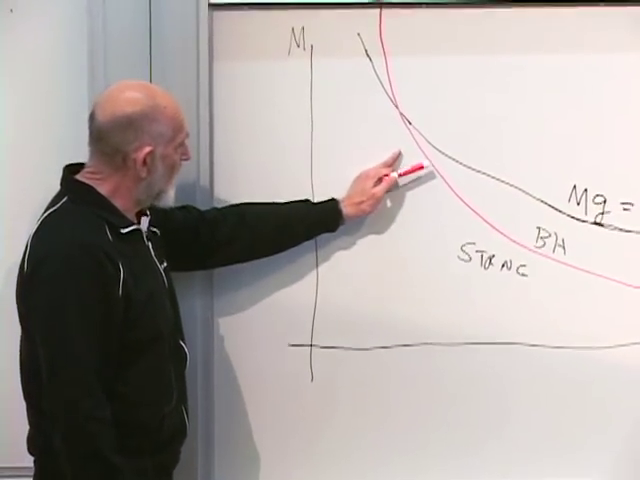
\includegraphics[width=0.70\textwidth]{lecture_07_figure_07.png}

\vspace{0.6em}
\begin{tikzpicture}[x=1cm,y=0.78cm]
  \draw[->] (0.4,0.4)--(7.0,0.4) node[right] {\(g_s\)};
  \draw[->] (0.4,0.4)--(0.4,6.5) node[above] {\(M\)};
  \draw[thick,black] plot[smooth] coordinates {(1.0,5.6) (1.5,4.0) (2.2,2.9) (3.2,2.1) (4.6,1.55) (6.3,1.2)};
  \draw[very thick,red!70!black] plot[smooth] coordinates {(1.25,6.0) (1.55,4.55) (2.0,3.15) (2.7,2.0) (3.8,1.25) (5.8,0.78)};
  \fill (2.05,3.1) circle (2pt) node[above right] {\((g_{s,*},M_*)\)};
  \node[black,rotate=-17] at (4.75,1.9) {\(Mg_s=M_0g_{s,0}\)};
  \node[red!70!black,rotate=-25] at (4.45,0.95) {\(Mg_s^2=1/\ell_s\)};
  \node at (5.75,3.5) {black hole};
  \node at (1.15,1.25) {string};
\end{tikzpicture}
\caption{黑板上的图及其整理后的解释。黑色绝热线与更陡的红色对应曲线相交于物体变为弦状的点。}
\lectureframe{00:49:35.000}
\end{figure}

在交点 \((M_*,g_{s,*})\) 处，两个方程为
\begin{align}
M_*g_{s,*} &= M_0g_{s,0}, \\
M_*g_{s,*}^2 &\sim \frac{1}{\ell_s}.
\end{align}
将第一个方程平方并除以第二个方程：
\begin{equation}
M_*
\sim M_0^2g_{s,0}^2\ell_s.
\end{equation}
乘以 \(\ell_s\)，
\begin{equation}
M_*\ell_s
\sim M_0^2g_{s,0}^2\ell_s^2
\sim M_0^2G_{N,0}.
\label{eq:l07-crossover-result}
\end{equation}

\begin{figure}[htbp]
\centering
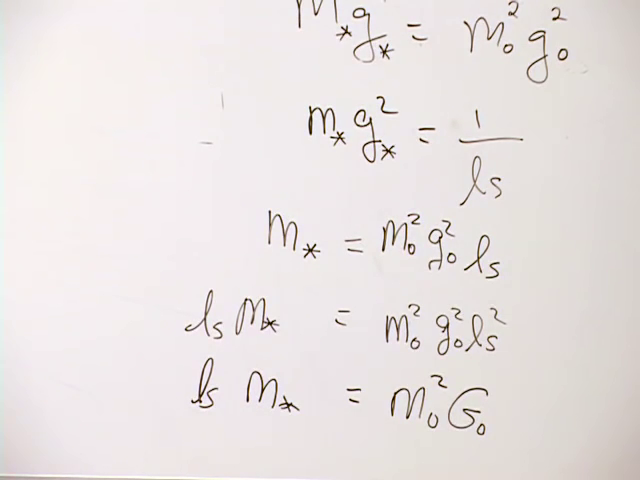
\includegraphics[width=0.68\textwidth]{lecture_07_figure_08.png}
\caption{完整的过渡代数，包括 \(M_*\ell_s=M_0^2g_{s,0}^2\ell_s^2=M_0^2G_{N,0}\)。}
\lectureframe{00:54:40.000}
\end{figure}

\begin{classroomqa}
\audiencequestion{当两个曲线方程相除时，\(\ell_s\) 最终应该在分子上还是分母上？\lecturetimestamp{00:52:41}}
\lecturerresponse{分子上。除以 \(1/\ell_s\) 相当于乘以 \(\ell_s\)，这就是为什么 \(M_*\sim M_0^2g_{s,0}^2\ell_s\)。}
\end{classroomqa}

在过渡点处弦公式成立，因此
\begin{equation}
S_*\sim M_*\ell_s.
\end{equation}
熵沿路径保持不变。将此陈述与方程~\eqref{eq:l07-crossover-result} 结合，得到原始目标黑洞的熵：
\begin{equation}
S_{\mathrm{BH}}(M_0)
\sim M_0^2G_{N,0}
\sim M_0^2\ell_{p,0}^2.
\label{eq:l07-final-correspondence}
\end{equation}
这就是所期望的面积律标度。

\section{对应关系证明了什么、没有证明什么}

这一构造并不是说原本强引力黑洞是一条自由弦。它把物体移到弦计数可信的区域，在那里读取熵，并沿可逆路径把该熵带回来。这一过渡是渐变而非位置明确的相边界，因此这一估计无法确定方程~\eqref{eq:l07-bh-exact} 中的系数 \(1/4\)。

尽管如此，同样的逻辑在参数意义上适用于带电黑洞、其他维度中的黑洞物体以及延展的黑膜。更对称和超对称的例子允许受保护的状态计数，在耦合变化时保留精确信息；那些方法能恢复数值系数，但增加了当前概念性论证所不需要的数学工具。

最重要的是，这一计算提供了微观解释。熵是隐藏结构的证据。流体力学描述密度、压强和流动，却省略了分子；流体的熵揭示出这类微观自由度存在。广义相对论同样描述视界而不展示其微观态。弦计数表明，一个自洽的量子引力理论可以包含足够多的态来解释黑洞熵。

\begin{classroomqa}
\audiencequestion{如果 \(S\sim M^3\ell_p^3\) 而不是二次结果，那会意味着什么？\lecturetimestamp{00:59:41}}
\lecturerresponse{那看起来会像体积律。房间里的普通物质或一杯咖啡的熵与体积成正比；二次答案之所以特殊，是因为通过 \(R_s\sim M\ell_p^2\)，它与视界面积成正比。}
\end{classroomqa}

这一结果是贝肯斯坦--霍金熵不仅仅是一种形式上的热力学类比的证据。它指向微观引力自由度，尽管基本推导并未逐个显现这些自由度。

\section{从最大熵到全息}

我们现在改变问题。不再询问指定状态的熵，而是询问与一个区域相容的最大熵。

从房间的普通点阵模型开始。将体积划分为大小为\(V_{\mathrm{cell}}\)的元胞，并让每个元胞携带一个是非问题：被占据还是空着。Susskind给这个假想原子起了一个故意荒谬的名字``meatonium''，以免任何现实的原子细节分散对计数的注意力。如果
\begin{equation}
N=\frac{V}{V_{\mathrm{cell}}},
\end{equation}
那么构型数和最大熵为
\begin{equation}
\Omega=2^N,
\qquad
S_{\max}=\log\Omega=N\log2
\sim\frac{V}{V_{\mathrm{cell}}}.
\label{eq:l07-volume-count}
\end{equation}

\begin{figure}[htbp]
\centering
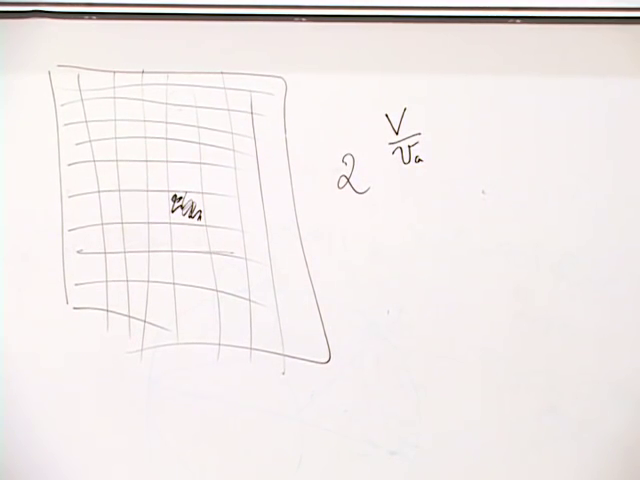
\includegraphics[width=0.68\textwidth]{lecture_07_figure_09.png}
\caption{房间被划分为元胞，每个元胞有两个状态。这计数的是最大熵，而不是班级所在的有序房间的熵。}
\lectureframe{01:05:20.000}
\end{figure}

实际房间远低于这个最大值。一个混沌地探索所有这些元胞选择的状态会极其炽热。从玩具模型中保留下来的是普通预期：独立自由度的数目，因而最大熵，随体积标度。

引力推翻了这一预期。考虑一个球形区域，其边界面积为\(A\)，初始熵为\(S_{\mathrm{i}}\)，质量为\(M\)，且小于恰好填满该球的黑洞质量\(M_{\mathrm{BH}}\)。如果\(M\)更大，其视界就已经延伸到所选边界之外。

现在送入一个质量为\(M_{\mathrm{BH}}-M\)的壳层。其组成无关紧要；讲座允许光、普通物质，甚至瑞士奶酪。安排它坍缩。最终状态是一个黑洞，其视界恰好填满该区域，熵为
\begin{equation}
S_{\mathrm{f}}=\frac{A}{4G_N}.
\end{equation}
第二定律要求
\begin{equation}
S_{\mathrm{i}}\le S_{\mathrm{f}}
=\frac{A}{4G_N}.
\label{eq:l07-holographic-bound}
\end{equation}

\begin{figure}[htbp]
\centering
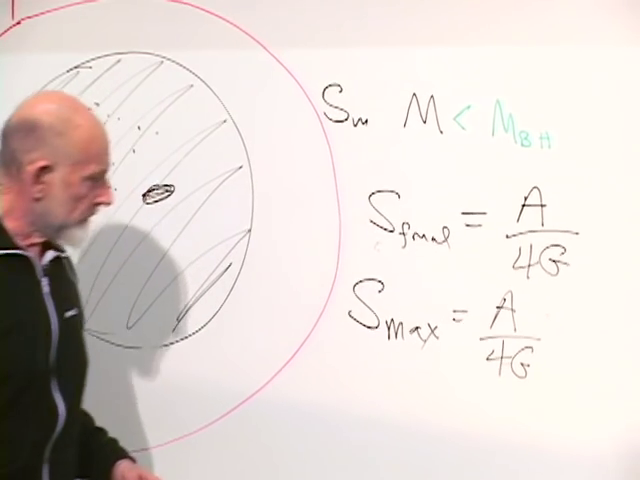
\includegraphics[width=0.70\textwidth]{lecture_07_figure_10.png}

\vspace{0.5em}
\begin{tikzpicture}[scale=0.88]
  \draw[thick] (0,0) circle (1.35);
  \draw[very thick,red!70!black] (0,0) circle (2.05);
  \fill[gray!25] (0,0) circle (1.32);
  \node at (0,0) {\(M,S_{\mathrm{i}}\)};
  \draw[-{Latex[length=3mm]},thick,red!70!black] (3.5,0)--(2.15,0);
  \node[align=center,right] at (3.5,0) {incoming shell\\\(M_{\mathrm{BH}}-M\)};
  \node[below] at (0,-2.2) {final horizon area \(A\)};
\end{tikzpicture}
\caption{壳层构造。足够的额外质量被向内送入，以形成一个视界恰好填满所选区域的黑洞。}
\lectureframe{01:13:30.000}
\end{figure}

因为该大小的黑洞是一个允许的状态并使不等式饱和，所以最大熵为
\begin{equation}
S_{\max}=\frac{A}{4G_N}.
\label{eq:l07-holographic-maximum}
\end{equation}
这就是计数形式的全息原理：引力区域中独立自由度的最大数目随其边界的面积标度，大约每个普朗克面积一个量级为一的自由度，而不是随内部普朗克体积的数目标度。\editorialnote{壳层论证假设该区域能够以所述方式被包围并坍缩。更一般的时空需要协变熵界，但球形论证捕捉了讲座中所用的原理。}

这种差异是巨大的。局域场论直觉表明，在不同内部点作出的选择应当独立组合，产生体积律。引力说，足够多的此类选择本身就会坍缩，而黑洞提供了更大的容许熵。因此，边界计数不是对体积计数的微小修正；它是希尔伯特空间的一种不同组织方式。

\begin{classroomqa}
\audiencequestion{对于一个密度大致均匀的极大宇宙，会发生什么？\lecturetimestamp{01:15:48}}
\lecturerresponse{这个问题需要宇宙学，而不是静态球形构造。它促使我们立即转向爱因斯坦方程的膨胀解。}
\end{classroomqa}

\begin{classroomqa}
\audiencequestion{面积界与不确定性原理有关吗？\lecturetimestamp{01:16:03}}
\lecturerresponse{讲座将这个问题留作开放，接下来转向宇宙学。}
\end{classroomqa}

\section{膨胀的空间}

我们在此不会从爱因斯坦方程推导宇宙学解；我们将写出这些解并学习如何解读它们。空间切片可以是正曲率且闭合的、负曲率且双曲的，或平坦的。就目前的讨论而言，取依赖于时间的时空中的空间平坦欧几里得切片。

\begin{classroomqa}
\audiencequestion{普通欧几里得空间的时空类似物是什么？\lecturetimestamp{01:19:37}}
\lecturerresponse{闵可夫斯基空间。这里考虑的宇宙学具有平坦空间切片，但不是闵可夫斯基时空，因为其空间度规随时间变化。}
\end{classroomqa}

熟悉的氣球圖像描述的是一個低一維的閉合膨脹曲面。Susskind 回憶曾用一個畫有標記的大氣球嘗試演示；記號筆削弱了橡膠，結果真的發出一聲爆響。這次意外也暴露了該類比中的一個概念缺陷。當普通氣球膨脹時，其橡膠分子彼此分離，材料變薄直至破裂。宇宙學空間並不會獲得被稀釋的局部定律。為保留該類比，必須想像不斷插入新的橡膠分子，使每個小塊都保持相同的局部性質。在平坦模型中，則將氣球換成一張被均勻向外拉伸並同樣得到補充的大薄片。

在數學上，膨脹體現在度規中：
\begin{equation}
\begin{aligned}
ds^2&=-dt^2+a(t)^2d\mathbf{x}^2,\\
d\mathbf{x}^2&=\delta_{ij}\,dx^i dx^j
=dx^2+dy^2+dz^2.
\end{aligned}
\label{eq:l07-frw-metric}
\end{equation}

\begin{figure}[htbp]
\centering
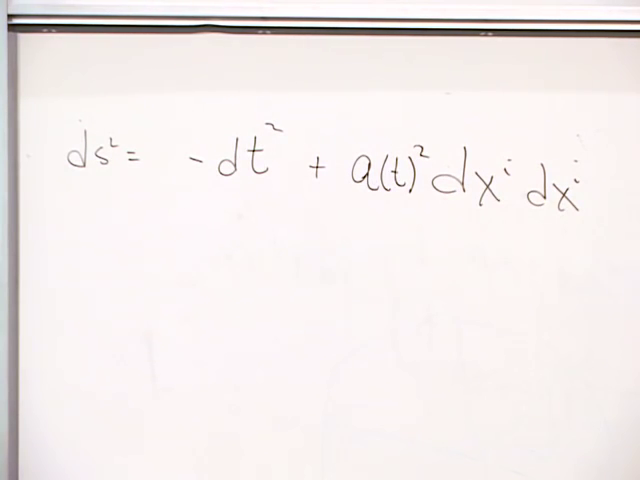
\includegraphics[width=0.72\textwidth]{lecture_07_figure_11.png}
\caption{黑板上寫出的空間平坦膨脹度規。}
\lectureframe{01:25:10.000}
\end{figure}

保持空間坐標固定的點稱為共動點。若兩個這樣的點具有坐標間隔 \(\Delta x\)，則它們在時刻 \(t\) 的固有距離為
\begin{equation}
D(t)=a(t)\Delta x.
\label{eq:l07-proper-distance}
\end{equation}
它們的坐標不動，但二者之間的度規距離發生變化。在固定 \(\Delta x\) 下求導，
\begin{equation}
V=\dot D=\dot a\,\Delta x
=\frac{\dot a}{a}D.
\end{equation}
定義哈勃參數
\begin{equation}
H(t)=\frac{\dot a(t)}{a(t)}.
\label{eq:l07-hubble-parameter}
\end{equation}
於是
\begin{equation}
V=H(t)D,
\label{eq:l07-hubble-law}
\end{equation}
這就是在固定宇宙時刻的哈勃定律。

\begin{figure}[htbp]
\centering
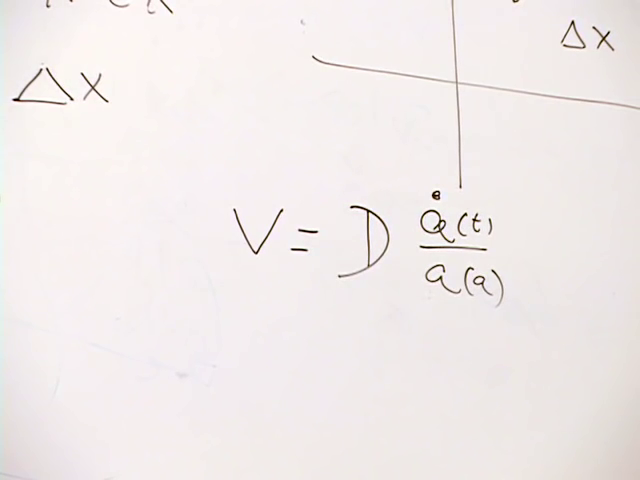
\includegraphics[width=0.68\textwidth]{lecture_07_figure_12.png}
\caption{黑板上寫出的等時退行定律：\(V=D\,\dot a/a\)。}
\lectureframe{01:29:10.000}
\end{figure}

``哈勃常數''這一名稱可能引起誤解。一般而言，\(H(t)\) 隨時間變化。真正在空間上恆定的是同一時間切片上每一對共動點的比值 \(V/D\)。

\begin{classroomqa}
\audiencequestion{對於遙遠星系，在此關係中出現的是哪個時刻？我們是在更早的時期觀測到它們的。\lecturetimestamp{01:31:10}}
\lecturerresponse{式~\eqref{eq:l07-hubble-law}是一個等時陳述。觀測沿著一條指向過去的光線進行，並在更早的時刻對遙遠星系取樣，因此測得的紅移與距離之間的關係需要完整的光錐歷史，而不是 \(H\) 的某一個瞬時值。}
\end{classroomqa}

\begin{figure}[htbp]
\centering
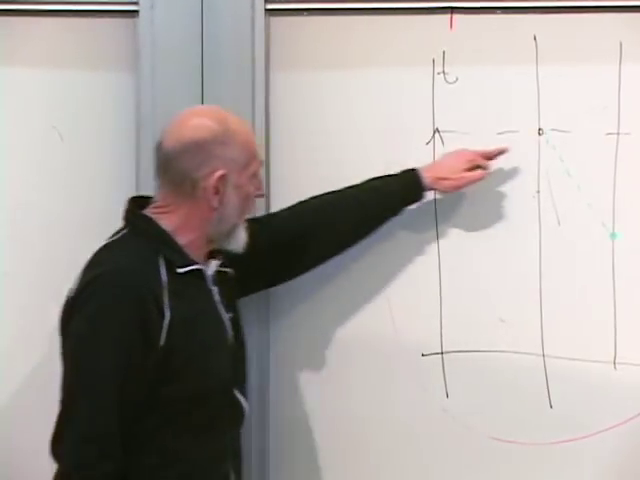
\includegraphics[width=0.66\textwidth]{lecture_07_figure_13.png}
\caption{用於區分等時間隔與觀測者沿過去光線所見的時空示意圖。}
\lectureframe{01:33:20.000}
\end{figure}

\section{哈勃尺度與德西特膨脹}

在單位 \(c=1\) 下，式~\eqref{eq:l07-hubble-law}給出退行速率為 1 的距離
\begin{equation}
D_H=\frac{1}{H}.
\label{eq:l07-hubble-radius}
\end{equation}
更遙遠的共動點可以有 \(V>1\)，甚至 \(V\gg1\)，而不違反狹義相對論。它們並非以超光速經過局部觀測者；它們的固有間隔增大，是因為其間的幾何本身在膨脹。\editorialnote{對於一般的隨時間變化的宇宙學，\(1/H\) 是哈勃半徑，並不自動是事件視界。在接下來討論的德西特情形中，它成為恆定的視界尺度。}

在許多較早的減速宇宙學模型中，\(H(t)\) 減小，而 \(1/H(t)\) 增大，因此曾經以超光速退行的區域後來可以進入因果接觸。講座中討論的晚期圖像則趨近於一個正常數 \(H\)。此時 \(1/H\) 保持固定，膨脹方程變為
\begin{equation}
\frac{\dot a}{a}=H,
\qquad
\dot a=Ha.
\label{eq:l07-constant-h}
\end{equation}

\begin{classroomqa}
\audiencequestion{恆定的哈勃參數的單位是什麼？\lecturetimestamp{01:38:24}}
\lecturerresponse{時間的倒數。等價地，取 \(c=1\) 時，它是長度的倒數。量 \(H^{-1}\) 同時提供了一個膨脹時間和一個距離尺度；講座使用了大約一百五十億年的數量級例子。}
\end{classroomqa}

式~\eqref{eq:l07-constant-h}的解為
\begin{equation}
a(t)=a_0e^{Ht}.
\label{eq:l07-desitter-scale-factor}
\end{equation}

\begin{classroomqa}
\audiencequestion{什麼函數的變化率與自身成正比？\lecturetimestamp{01:39:04}}
\lecturerresponse{指數函數。因此標度因子為 \(a_0e^{Ht}\)，而度規中的空間係數 \(a(t)^2\) 按 \(e^{2Ht}\) 增長。}
\end{classroomqa}

\begin{figure}[htbp]
\centering
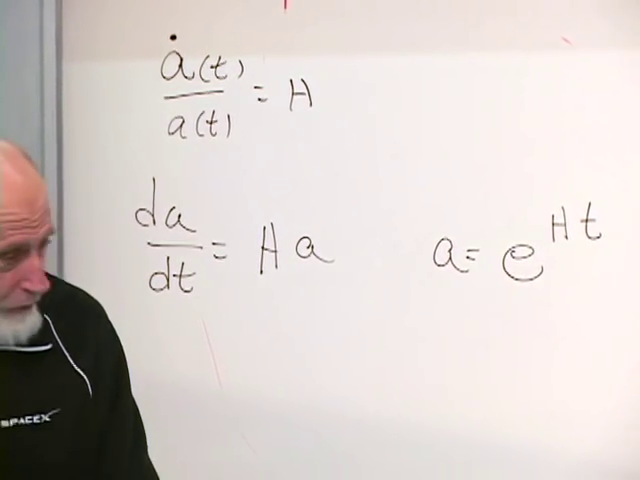
\includegraphics[width=0.70\textwidth]{lecture_07_figure_14.png}
\caption{黑板上寫出的常 \(H\) 方程及其指數解。}
\lectureframe{01:39:30.000}
\end{figure}

具有這種指數膨脹的時空是德西特空間。其恆定的哈勃尺度在有限固有距離處產生一個事件視界。該幾何在某種意義上是黑洞圖像的互補：觀測者始終處於一個宇宙學視界之內，而足夠遙遠的物體退行，永遠無法發出信號追上該觀測者。黑洞視界對外部觀測者隱藏內部；德西特視界則對觀測者隱藏其可及區域的外部。與普通蒸發黑洞不同，這裡將理想的德西特幾何視為持續存在。這一比較才剛剛開始。下一講將展開視界、其熱力學以及它為宇宙學帶來的種種疑難。
\chapter{真空能量与德西特视界}

\lectureoverview{真空能量不同于普通物质：它既不选出一个优先的惯性系，也不随宇宙膨胀而稀释。一旦把引力纳入进来，这个表面上无害的能量零点就会改变时空的几何。我们将推导物质主导的规律\(a(t)\propto t^{2/3}\)，将其与真空主导的规律\(a(t)\propto e^{Ht}\)进行对比，然后在共形坐标中重写德西特时空。由此得到的因果图揭示出一个依赖于观测者的、位于固定固有距离处的事件视界。}

\section{真空中的量子涨落}

我们从激发整场讲座的问题开始。量子场论赋予空无一物的空间以能量。这是否意味着真实的电子--正电子对会不断地从虚无中涌现出来？

\begin{classroomqa}
\audiencequestion{电子--正电子对的产生与湮灭真的在真空中发生吗，还是说那只不过是一种记账手段？\lecturetimestamp{00:00:06}}
\lecturerresponse{虚粒子对会对真空能量有所贡献，但它们并不是那种能够被观察到从空无一物的空间中涌现出来的普通粒子。它们是量子基态的涨落，并且只在适合虚过程的限度内持续存在。}
\end{classroomqa}

谐振子给出了最干净的模型。经典地看，它可以静止在其势能的最小值处。量子力学地看，精确地位于最小值处与精确地具有零动量是不相容的。基态在两者之间做出折中，并保留零点能
\begin{equation}
E_0=\frac{1}{2}\hbar\omega.
\label{eq:l08-zero-point}
\end{equation}
这是谐振子所能具有的最低能量。它不是激发态，也不代表一股可观测的粒子流。

自由场分解为简正模，每个模都像一个谐振子那样运动。腔中的电磁场就是一个熟悉的例子。每个模都贡献一个形如式~\eqref{eq:l08-zero-point}中的项；电子、夸克以及其他量子场则贡献它们各自的基态涨落。把这些贡献加起来，就得到我们所谓的真空能量。朴素的微观估计与观测到的宇宙学尺度之间那臭名昭著的不匹配是真实存在的，但它不是本讲的主题。

\begin{classroomqa}
\audiencequestion{大约\(120\)个数量级的差异还会再讨论吗？\lecturetimestamp{00:02:59}}
\lecturerresponse{不在这里讨论。当前的目标是理解宇宙学视界：宇宙学方程如何产生加速膨胀，以及为什么加速膨胀会产生事件视界。}
\end{classroomqa}

\begin{classroomqa}
\audiencequestion{上一讲中的紫外--红外关系是今晚讨论的一部分吗？\lecturetimestamp{00:03:59}}
\lecturerresponse{它以后可能会被重新讨论，但它不是计划中论证的一部分。眼下的路径是从真空能量到宇宙学，然后再到视界。}
\end{classroomqa}

\section{为什么真空能量是洛伦兹不变的}

下一个问题看起来很简单，却揭示出真空能量的定义性属性。如果空无一物的空间具有正的能量密度，为什么它不像光学介质那样起作用并改变光速？

\begin{classroomqa}
\audiencequestion{正的真空能量密度难道不应该产生折射效应，使光传播得稍微慢一些吗？\lecturetimestamp{00:04:35}}
\lecturerresponse{普通物质能够做到这一点，是因为它定义了一个优先的静止系。真空能量则不同：它不选出这样一个系，而且每个惯性观测者都得到相同的真空能量密度。因此对光的局域测量仍然保持不变的速度\(c\)。}
\end{classroomqa}

我们必须把定律的对称性与某个特定状态的对称性区分开来。物理方程可以是平移不变的，尽管斯坦福不是伯克利，地球也不是星际空间。平移\emph{整个}物理安排会使定律保持不变；而物质的实际安排不必在每个位置看起来都一样。同样地，旋转不变的方程并不会使这间教室具有旋转对称性。

同样的区分也适用于洛伦兹变换。气体有一个静止系。穿过它运动的观测者会看到运动的分子和不同的能量密度，因此气体的状态不是洛伦兹不变的，尽管支配它的方程是洛伦兹不变的。普通物质、辐射浴以及实验室装置都通过选出特殊的运动或方向而破坏了这一对称性。

真空能是不这样做的物质的例外形式。设想一个报告真空能密度的探测器。它在静止时给出某个值\(\rho_{\rm vac}\)。加速探测器并重复测量：结果不变。在相对论记号中，这一性质由与度规成正比的应力张量编码，
\begin{equation}
T_{\mu\nu}^{\rm vac}=-\rho_{\rm vac}g_{\mu\nu},
\qquad
p_{\rm vac}=-\rho_{\rm vac}.
\label{eq:l08-vacuum-stress}
\end{equation}
\editorialnote{压强关系并非在黑板上推导出来的。它是讲座中两个定义性质——洛伦兹不变性和膨胀过程中密度恒定——背后的协变陈述。}

局域这一限定很重要。经过观察者的光线用附近的钟和尺测量，其运动速率为\(c\)。在膨胀几何中询问遥远光线相对于我们的速度，需要选择坐标以及比较遥远事件的方案。该坐标速度不必等于\(c\)，尽管每个局域观察者都测得\(c\)。

\begin{classroomqa}
\audiencequestion{在这次讨论中，真空能和宇宙学常数是同义词吗？\lecturetimestamp{00:11:57}}
\lecturerresponse{是的。它们是同一个项在爱因斯坦方程中的两种放置方式：它可以被描述为几何侧的宇宙学常数，或被描述为源侧的洛伦兹不变真空应力能量。}
\end{classroomqa}

\section{什么会稀释，什么不会}

用质量为\(m\)的非相对论性粒子充满一个大区域。在足以对星系和星系团取平均的大尺度上，假设分布是均匀的。如果一个共动体积包含\(N\)个粒子，其物质密度为
\begin{equation}
\rho_m=\frac{Nm}{V}.
\end{equation}
当每个线度加倍时，体积增大\(2^3=8\)，而\(N\)和\(m\)保持不变。因此密度降至其先前值的八分之一。普通物质会稀释，因为同样的粒子占据更大的物理体积。

辐射也会稀释，而且更快。其数密度随体积下降，同时每个光子的波长被拉伸，其能量发生红移。我们稍后将记录结果\(\rho_r\propto a^{-4}\)，但今晚我们不会求解辐射主导的宇宙学。

真空能是例外：
\begin{equation}
\rho_{\rm vac}(t)=\text{constant}.
\label{eq:l08-rho-vac-constant}
\end{equation}
它不会成团，不会选择方向，不会选择惯性系，也不会随着空间膨胀而变得稀薄。如果一个共动盒子增大，其中包含的真空能按体积成比例增大。

\editorialnote{密度恒定并不意味着膨胀的共动盒子内部的总真空能恒定。协变应力能量守恒，
\(\dot\rho+3H(\rho+p)=0\)，之所以得到满足，是因为真空能具有负压强\(p_{\rm vac}=-\rho_{\rm vac}\)。功项恰好提供了盒子总真空能的变化。}

\section{引力看到能量的零点}

在非引力的实验室物理中，将每个能量都移动同一个常数通常不改变任何东西。光谱依赖于差值：激发态原子与未激发原子之间的能量，或者有粒子与无粒子的状态之间的能量。真空似乎不提供任何可以据以测量其绝对能量的参照。

引力改变了问题。质量就是能量，能量产生引力，因此真空能会产生引力。一个在原子跃迁中不可见的常数可以弯曲时空。

爱因斯坦方程将几何与源分开：
\begin{equation}
G_{\mu\nu}=8\pi G_N T_{\mu\nu},
\label{eq:l08-einstein}
\end{equation}
其中单位取\(c=1\)。爱因斯坦张量\(G_{\mu\nu}\)由度规\(g_{\mu\nu}(x)\)及其导数构成。应力张量\(T_{\mu\nu}\)包含来自物质和非引力场的能量密度、动量密度、压强和应力。真空能正如普通物质一样属于这个源侧。\editorialnote{口头介绍简要地将\(8\pi/3\)与张量方程联系起来。因子\(1/3\)属于下面的空间平坦弗里德曼方程，而不属于方程~\eqref{eq:l08-einstein}。}

\begin{figure}[htbp]
\centering
\includegraphics[width=0.62\textwidth]{lecture_08_figure_02.png}
\caption{爱因斯坦方程的几何侧，由时空度规\(g_{\mu\nu}(x)\)构成。}
\lectureframe{00:21:58.820}
\end{figure}

\section{几何被约化为一个标度因子}

我们现在选择具有平坦空间切片的最简单的均匀膨胀几何：
\begin{equation}
ds^2=-dt^2+a(t)^2\,d\mathbf{x}^2,
\qquad
d\mathbf{x}^2=dx^2+dy^2+dz^2.
\label{eq:l08-frw-metric}
\end{equation}
坐标标记\(\mathbf{x}\)被画在一张无限的橡胶片上。它们不必移动，但它们的物理间距会移动。相隔\(\Delta\mathbf{x}\)的两个共动点在固定\(t\)时的固有距离为
\begin{equation}
D(t)=a(t)\lvert\Delta\mathbf{x}\rvert.
\label{eq:l08-proper-distance}
\end{equation}
因此，这个高度对称几何的所有时间依赖性都储存在一个函数中，即标度因子\(a(t)\)。常数\(a\)在空间重标度后给出平坦的闵可夫斯基时空。依赖于时间的\(a\)可以使每个空间切片保持平坦，同时使整个时空弯曲。

\begin{classroomqa}
\audiencequestion{对于坐标标记\(x=7\)和\(x=13\)，它们的坐标间隔是否为\(4\)？\lecturetimestamp{00:27:40}}
\lecturerresponse{不是。它是\(13-7=6\)，因此它们的物理间隔为\(6a(t)\)。这一修正很有用：\(x\)标记共动位置，而乘以\(a(t)\)则给出物理距离。}
\end{classroomqa}

对于该度规和空间均匀的能量密度，爱因斯坦方程的一个分量成为空间平坦的弗里德曼方程，
\begin{equation}
\left(\frac{\dot a}{a}\right)^2
=\frac{8\pi G_N}{3}\rho(t).
\label{eq:l08-friedmann}
\end{equation}
比值
\begin{equation}
H(t)\equiv\frac{\dot a(t)}{a(t)}
\label{eq:l08-hubble-definition}
\end{equation}
即为哈勃参数。在此阶段它是一个定义，并且可以随时间变化。

\begin{figure}[htbp]
\centering
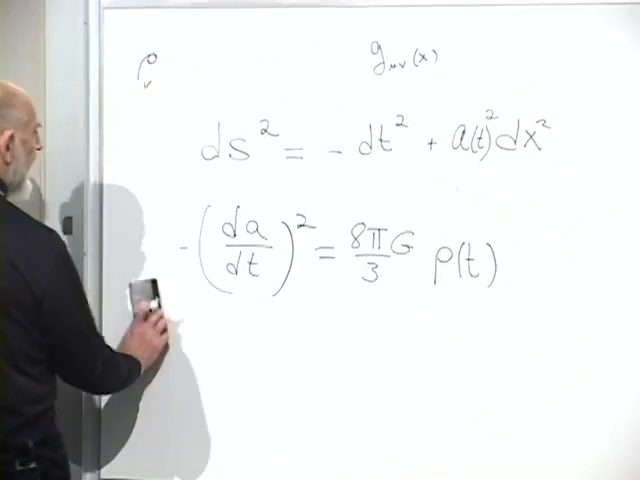
\includegraphics[width=0.90\textwidth]{lecture_08_figure_03.png}
\caption{在板上补回缺失的因子\(1/a^2\)之后的平坦膨胀度规和弗里德曼方程。}
\lectureframe{00:30:30.000}
\end{figure}

\paragraph{能量平衡图像。}
对于这一能量平衡图像，方程~\eqref{eq:l08-friedmann}被示意性地写为
\begin{equation}
-\frac{3}{8\pi G_N}H^2+\rho=0.
\label{eq:l08-energy-heuristic}
\end{equation}
物质能量为正，而由膨胀标度因子代表的引力自由度带有负的动能项。在这个约化问题中，负的引力能加上正的物质量能等于零是一个有用的助记。

\editorialnote{方程~\eqref{eq:l08-energy-heuristic}是高度对称的微超空间模型中的哈密顿约束，而不是一个坐标无关的定理，断言每一个任意宇宙都具有等于零的全局守恒总能量。讲座将其用作对弗里德曼约束的启发式解释。}

\section{物质主导的膨胀}

回到一个共动数学盒子，其坐标边长为\(\Delta x=1\)。它的物理边长为\(a(t)\)，因此其物理体积为\(a(t)^3\)。如果它包含\(N\)个质量为\(m\)的非相对论性粒子，那么
\begin{equation}
\rho_m(t)=\frac{Nm}{a(t)^3}
=\frac{\rho_0}{a(t)^3}.
\label{eq:l08-matter-density}
\end{equation}
粒子本身并不膨胀；膨胀的是它们的平均间距。

\begin{figure}[htbp]
\centering
\includegraphics[width=0.84\textwidth]{lecture_08_figure_04.png}
\caption{在组装共动盒子论证时的度规和弗里德曼方程。}
\lectureframe{00:36:07.940}
\end{figure}

代入方程~\eqref{eq:l08-friedmann}得到
\begin{equation}
\left(\frac{\dot a}{a}\right)^2
=\frac{8\pi G_N\rho_0}{3a^3}.
\end{equation}
记\(K=8\pi G_N\rho_0/3\)并选择膨胀分支：
\begin{align}
\dot a^2&=\frac{K}{a},\\
\dot a&=\sqrt{K}\,a^{-1/2},\\
a^{1/2}\,da&=\sqrt{K}\,dt.
\label{eq:l08-matter-separated}
\end{align}

\begin{classroomqa}
\audiencequestion{分离后的方程应如何求解？\lecturetimestamp{00:38:15}}
\lecturerresponse{对两边积分。\(a^{1/2}\,da\)的积分是\(\frac{2}{3}a^{3/2}\)，而不是\(\frac{3}{2}a^{3/2}\)；\(\frac{3}{2}\)是新的幂次，而\(\frac{2}{3}\)是系数。}
\end{classroomqa}

因此，
\begin{equation}
\frac{2}{3}a^{3/2}
=\sqrt{K}\,(t-t_B),
\end{equation}
其中\(t_B\)是确定所选时间原点的积分常数。除归一化和时间平移外，
\begin{equation}
a(t)\propto (t-t_B)^{2/3}.
\label{eq:l08-matter-solution}
\end{equation}

\begin{figure}[htbp]
\centering
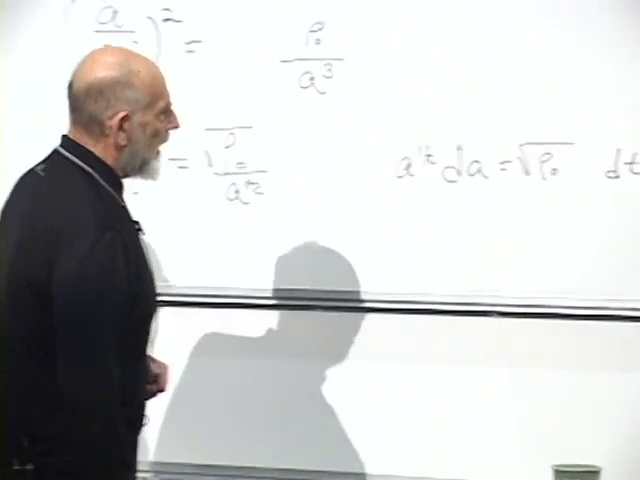
\includegraphics[width=0.86\textwidth]{lecture_08_figure_05.png}
\caption{物质密度代入和变量分离导致\(a^{1/2}da\propto dt\)。}
\lectureframe{00:38:30.000}
\end{figure}

曲线\(t^{2/3}\)比直线增长得更慢。其斜率减小，因此物质主导的宇宙减速。在讲座所用的牛顿语言中，粒子起初彼此分离，而它们之间的相互引力吸引不断降低分离的速率。

\begin{figure}[htbp]
\centering
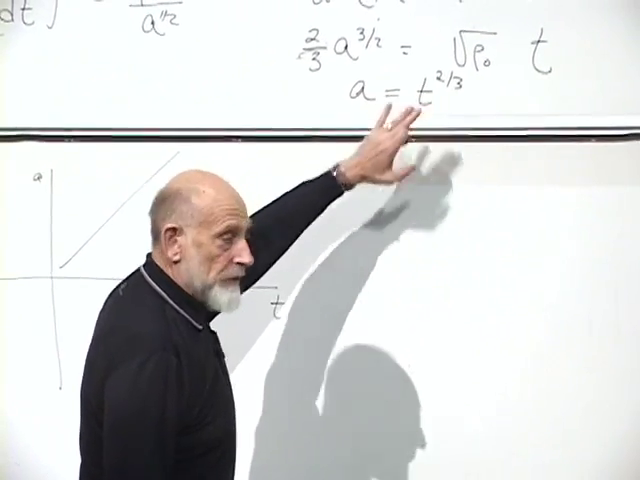
\includegraphics[width=0.86\textwidth]{lecture_08_figure_06.png}
\caption{板上对线性膨胀与向下凹的物质定律\(a(t)\propto t^{2/3}\)的比较。}
\lectureframe{00:40:00.000}
\end{figure}

为了定位，辐射浴有
\begin{equation}
\rho_r\propto a^{-4},
\end{equation}
而不是\(a^{-3}\)：体积稀释贡献三个幂次，宇宙学红移再贡献一个。相应的标度因子也可以求解，但讲座有意将这一练习搁置一旁。

\section{真空主导的膨胀}

现在只在弗里德曼方程右侧放真空能。由于\(\rho_{\rm vac}\)是常数，
\begin{equation}
\left(\frac{\dot a}{a}\right)^2
=\frac{8\pi G_N}{3}\rho_{\rm vac}
\equiv H^2.
\label{eq:l08-de-sitter-friedmann}
\end{equation}
\(H\)有两种用法需要区分开。方程~\eqref{eq:l08-hubble-definition}定义了可能随时间变化的量\(\dot a/a\)。方程~\eqref{eq:l08-de-sitter-friedmann}说明，在纯真空能宇宙中它的值是常数
\begin{equation}
H=\sqrt{\frac{8\pi G_N\rho_{\rm vac}}{3}}.
\end{equation}
取膨胀分支得到
\begin{equation}
\dot a=Ha,
\end{equation}
因此
\begin{equation}
a(t)=C e^{Ht}.
\label{eq:l08-exponential-solution}
\end{equation}
积分常数\(C\)确定共动坐标的任意归一化。正比于\(a\)当前值的增长是指数增长。

\begin{figure}[htbp]
\centering
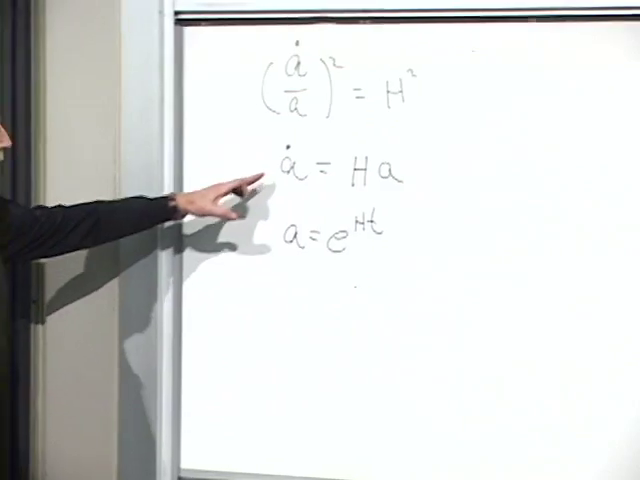
\includegraphics[width=0.88\textwidth]{lecture_08_figure_07.png}
\caption{真空主导的方程\((\dot a/a)^2=H^2\)、它的一阶形式\(\dot a=Ha\)以及指数解。}
\lectureframe{00:47:45.000}
\end{figure}

共动物体的哈勃定律为
\begin{equation}
v_{\rm rec}=HD.
\label{eq:l08-hubble-law}
\end{equation}
在这个纯德西特情形中，退行速率等于\(c\)处的固有距离是常数：
\begin{equation}
D_H=\frac{c}{H},
\label{eq:l08-hubble-radius}
\end{equation}
或在板上所用的\(c=1\)单位下为\(D_H=H^{-1}\)。这个固定尺度将作为德西特事件视界半径在几何上重新出现。\editorialnote{哈勃半径在任意随时间变化的宇宙学中并不自动是事件视界。这一等同在这里成立，是因为在精确德西特空间中\(H\)是常数。}

本讲提出了一个用于真空能探测器的思想实验。将两个极轻的检验物体置于远离其他源的地方，初始时相对于共动流静止，并使它们之间的相互吸引可以忽略。它们的间距遵循指数膨胀。该效应对于地面装置来说实在太小，但宇宙尺度的距离和回溯时间使得同样的物理过程可以被观测到。

\section{从物质主导到真空主导}

本讲所考虑的真实宇宙学模型包含两项：
\begin{equation}
H(t)^2
=\frac{8\pi G_N}{3}
\left(\frac{\rho_0}{a(t)^3}+\rho_{\rm vac}\right).
\label{eq:l08-mixed-friedmann}
\end{equation}
在\(a\)较小时，由于\(a^{-3}\)很大，物质项占主导，解类似于\(t^{2/3}\)。随着宇宙增长，物质被稀释，而真空能保持固定。最终常数项胜出，标度因子向上弯折趋向\(e^{Ht}\)。

\begin{figure}[htbp]
\centering
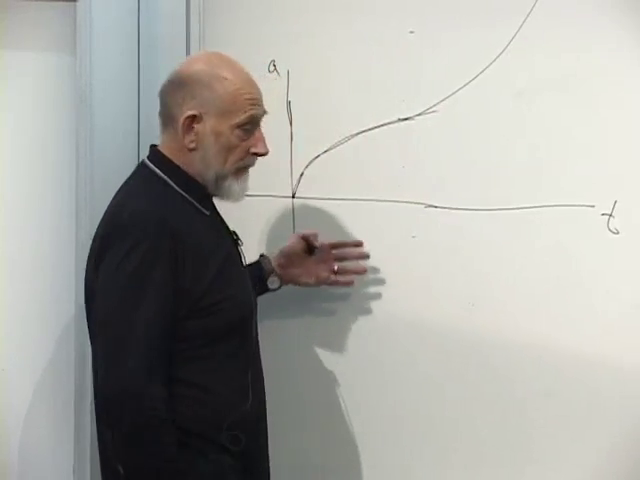
\includegraphics[width=0.87\textwidth]{lecture_08_figure_08.png}
\caption{本讲所描绘的定性转变：早期物质主导的减速，随后是晚期真空主导的指数增长。}
\lectureframe{00:53:30.000}
\end{figure}

\begin{classroomqa}
\audiencequestion{指数解包含一个积分常数。我们怎么知道它不是极其微小？\lecturetimestamp{00:52:41}}
\lecturerresponse{我们测量它。向宇宙更远处看意味着向更早的过去看，因此不同距离上的观测重建的是膨胀曲线较早的部分，而不仅仅是它今天的值。}
\end{classroomqa}

本讲报告说，当时可获得的晚期观测在约百分之五的水平上与指数分支一致，并将这些证据描述为令人信服的，尽管不如电子性质那样的精密测量那样精确。这应被理解为本讲的历史评估，而非当今的精密陈述。

\begin{classroomqa}
\audiencequestion{向上弯折的膨胀曲线最终是否会阻止我们将观测追溯到宇宙大爆炸或宇宙微波背景？\lecturetimestamp{00:55:05}}
\lecturerresponse{这不是作为外推图形的问题来探讨的。相关的、不变量意义上的问题是事件视界的存在性，而这正是我们现在转向的因果问题。}
\end{classroomqa}

\section{束缚系统与遥远未来}

如果指数膨胀持续下去，每一个被稀释的成分与\(\rho_{\rm vac}\)相比都变得可以忽略。这并不意味着原子、太阳系或星系本身被拉伸开来。被束缚得足够强而保持束缚的系统不遵循哈勃流。

\begin{classroomqa}
\audiencequestion{今天没有在膨胀的星系，当真空能占主导时最终会膨胀吗？\lecturetimestamp{00:57:44}}
\lecturerresponse{束缚系统保持束缚。银河系和仙女座星系属于将保持在一起的近邻结构，而已经随膨胀运动的足够遥远的星系继续向外运动，最终越过我们的视界。}
\end{classroomqa}

\emph{被吸引}与\emph{被束缚}之间的区分至关重要。以超过逃逸速度发射的火箭仍然处于地球的吸引引力之下，然而它不会返回。同样，普通引力吸引可能是两个星系之间最大的局域力，而它们的相对轨道却未必是束缚的。

\begin{classroomqa}
\audiencequestion{我们的星系在引力上与一个星系群相关联。加速膨胀最终会克服那种吸引吗？\lecturetimestamp{00:59:17}}
\lecturerresponse{只有局域结构中真正束缚的部分会保持在一起。作为一个描述性标签的星系团是不够的；束缚意味着相对运动低于逃逸。更遥远的星系可以被吸引，却仍然以超过逃逸速度退行。}
\end{classroomqa}

为了直观理解，本讲将相对径向加速度示意性地表示为一个吸引的平方反比项加上一个与间距成正比的真空项：
\enlargethispage{2pt}
\begin{equation}
\ddot r\sim-\frac{G_NM}{r^2}+H^2r.
\label{eq:l08-newtonian-vacuum}
\end{equation}
在理想化的德西特极限下，这些系数与时间无关。第二项之所以增长，仅仅是因为\(r\)增长；它并非源于\(G_N\)的逐渐减弱。

\editorialnote{方程~\eqref{eq:l08-newtonian-vacuum}是一个牛顿式的相对加速度启发式表述，而不是广义相对论中额外的基本力定律。在精确的德西特空间中，相邻的自由下落世界线的相对加速度正比于\(H^2r\)。}

\begin{figure}[htbp]
\centering
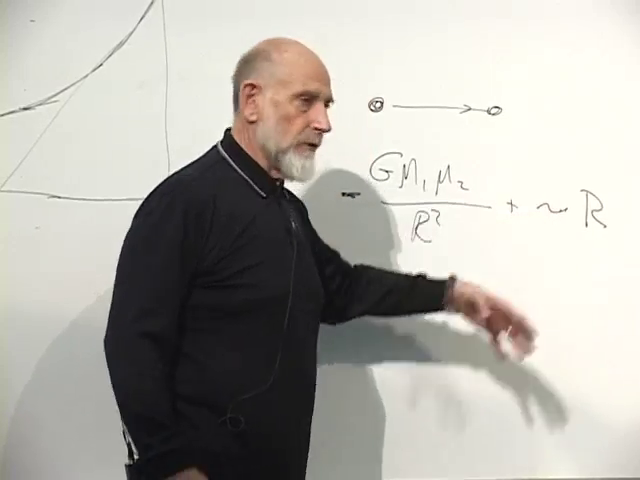
\includegraphics[width=0.88\textwidth]{lecture_08_figure_09.png}
\caption{黑板上对平方反比吸引与随间距线性增长的有效真空排斥之间的比较。}
\lectureframe{01:04:10.000}
\end{figure}

\begin{classroomqa}
\audiencequestion{向外的效应本身会随时间增大吗？\lecturetimestamp{01:01:18}}
\lecturerresponse{在固定间距下不会。其系数是常数。自由退行的物体彼此越来越远，于是正比于\(r\)的项因距离更大而更大。}
\end{classroomqa}

\begin{classroomqa}
\audiencequestion{能否把净效应描述为牛顿常数逐渐减小？\lecturetimestamp{01:02:30}}
\lecturerresponse{不能。\(G_N\)保持常数。在指定间距下，两个系数都不变；随距离改变的只是\(1/r^2\)吸引与正比于\(r\)的项之间的相对重要性。}
\end{classroomqa}

\begin{classroomqa}
\audiencequestion{在真空能变得重要之前的早期宇宙中，同样的星系是否受引力束缚？\lecturetimestamp{01:05:03}}
\lecturerresponse{普通吸引占主导本身并不蕴含束缚。许多星系当时已经在以逃逸速率或更高的速率彼此分离。真空能后来决定大尺度膨胀是减速趋向再坍缩还是加速远离，但最大力与束缚轨道仍是不同的陈述。}
\end{classroomqa}

因此，遥远未来的观测者可能生活在一个已经并合的局部结构中，而每一个未束缚的星系都已变得不可观测。若没有历史记录，该观测者可以有理由地推断宇宙几乎空无一物。这种因果上的孤独，而非局部物体的毁灭，才是通向视界的物理前导。

\section{事件视界的含义}

在破缺之后，令
\begin{equation}
a(t)=e^{Ht}
\end{equation}
并将度规写为
\begin{equation}
ds^2=-dt^2+e^{2Ht}d\mathbf{x}^2.
\label{eq:l08-de-sitter-metric}
\end{equation}

\begin{classroomqa}
\audiencequestion{这个度规所描述的时空叫什么名字？\lecturetimestamp{01:08:13}}
\lecturerresponse{它是德西特时空，通常简称为德西特空间。其视界之所以重要，是因为真空主导的宇宙在晚期趋近于这一几何。}
\end{classroomqa}

在画出其因果结构之前，先回顾彭罗斯图的作用。无穷区间被压缩到一幅有限的图中，而零射线仍保持在\(45^\circ\)。在平直时空中，有质量物体终止于未来类时无穷，零射线终止于零无穷，而一个被允许任意长久等待的惯性观测者没有事件视界排除某个永久的时空区域。

\begin{figure}[htbp]
\centering
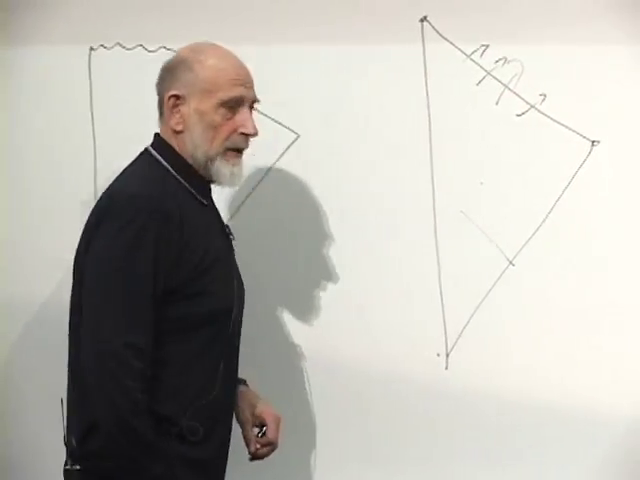
\includegraphics[width=0.80\textwidth]{lecture_08_figure_10.png}
\caption{在引入视界之前，用来区分类时与零终点的平直时空彭罗斯图。}
\lectureframe{01:10:35.000}
\end{figure}

黑洞图提供了对照。外部观测者只能接收来自该观测者未来世界线因果过去的信号。即使观测时间趋于无穷，内部区域仍被排除。能与该观测者通信的事件与永远不能通信的事件之间的边界，就是事件视界。

\begin{definition}
观测者的事件视界是那些事件所成集合的边界：从这些事件出发，未来指向的因果信号能够到达该观测者的世界线。
\label{def:l08-event-horizon}
\end{definition}

\begin{figure}[htbp]
\centering
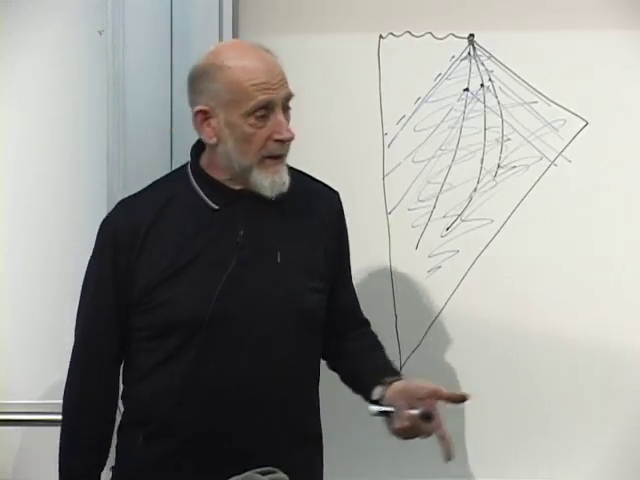
\includegraphics[width=0.80\textwidth]{lecture_08_figure_11.png}
\caption{与黑洞的对照：来自任意晚的外部观测的后向光锥永远不包含事件视界之外的区域。}
\lectureframe{01:13:50.000}
\end{figure}

因此，事件视界是一个全局因果边界，而不仅仅是某个物体今天恰好看起来暗淡的距离。要确定它的位置，必须知道即使经过任意长久的等待，哪些信号仍能到达。

\section{压缩无穷未来}

方程~\eqref{eq:l08-de-sitter-metric}中的空间坐标已经覆盖一个无穷平直切片。我们将不动它们，只压缩时间。引入共形时间\(T\)，要求
\begin{equation}
dt^2=e^{2Ht}dT^2.
\label{eq:l08-conformal-definition}
\end{equation}
取未来指向的平方根并整理，得到
\begin{equation}
dT=e^{-Ht}dt.
\end{equation}

\begin{classroomqa}
\audiencequestion{这个积分是什么，包括其符号？\lecturetimestamp{01:17:25}}
\lecturerresponse{它是\(-H^{-1}e^{-Ht}\)。一个加性常数只是平移\(T\)的原点，因此选择它使无穷未来位于\(T=0\)。}
\end{classroomqa}

因此
\begin{equation}
T=-\frac{1}{H}e^{-Ht},
\qquad -\infty<T<0.
\label{eq:l08-conformal-time}
\end{equation}
当\(t\to-\infty\)时，\(T\to-\infty\)。当固有时\(t\to+\infty\)时，\(T\to0^{-}\)。无穷未来已被置于有限的水平线\(T=0\)上；没有观测者在有限固有时内到达它。

\begin{figure}[htbp]
\centering
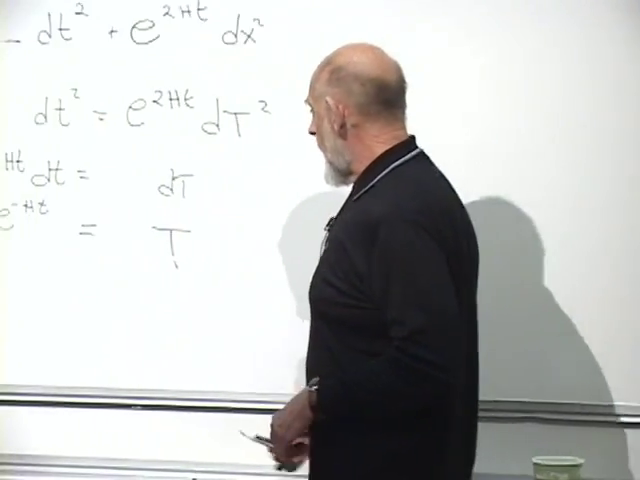
\includegraphics[width=0.86\textwidth]{lecture_08_figure_12.png}
\caption{共形时间积分以及无穷未来\(t\to+\infty\)到\(T=0^{-}\)的映射。}
\lectureframe{01:19:10.000}
\end{figure}

由方程~\eqref{eq:l08-conformal-time}，
\begin{equation}
HT=-e^{-Ht},
\qquad
e^{2Ht}=\frac{1}{H^2T^2}.
\label{eq:l08-conformal-factor}
\end{equation}
将\(dt=e^{Ht}dT\)用于方程~\eqref{eq:l08-de-sitter-metric}，便得到
\begin{equation}
ds^2=\frac{1}{H^2T^2}
\left(-dT^2+d\mathbf{x}^2\right).
\label{eq:l08-conformal-metric}
\end{equation}
括号中的表达式是闵可夫斯基度规。现在，全部德西特几何都位于一个共同的共形因子中，该因子在\(T\to0^{-}\)时发散。

\begin{figure}[htbp]
\centering
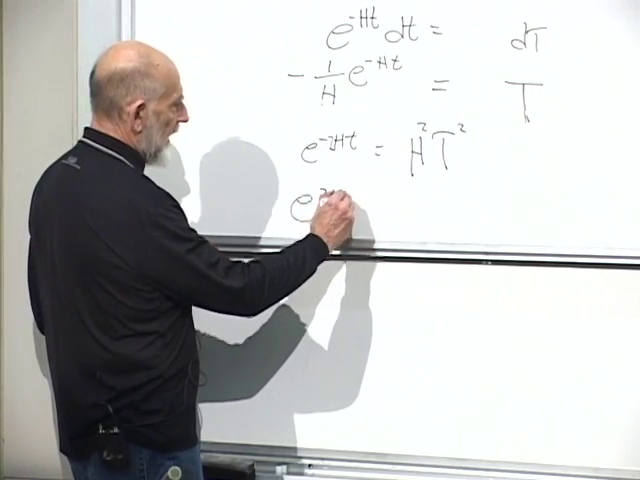
\includegraphics[width=0.87\textwidth]{lecture_08_figure_13.png}
\caption{将\(e^{2Ht}\)与\(1/(H^2T^2)\)联系起来的代数，为度规的共形形式作准备。}
\lectureframe{01:22:50.000}
\end{figure}

\begin{classroomqa}
\audiencequestion{在这个度规中，什么条件决定了光线的路径？\lecturetimestamp{01:23:49}}
\lecturerresponse{光线沿零路径传播，\(ds^2=0\)。因此共同的共形因子相消，沿选定的空间方向留下\(dT=\pm dx\)。}
\end{classroomqa}

在\((T,x)\)图中，光线是\(45^\circ\)的直线：
\begin{equation}
\frac{dx}{dT}=\pm1.
\label{eq:l08-null-lines}
\end{equation}
坐标图在\(T=0\)附近被高度压缩，但它恰好保留了我们需要的信息：哪些事件能够通信。

\begin{figure}[htbp]
\centering
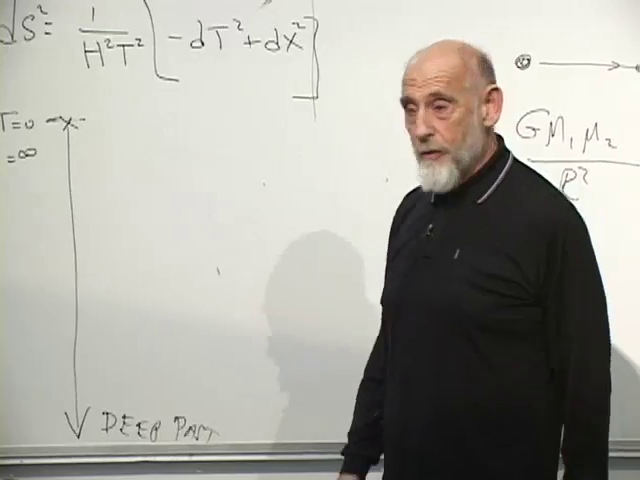
\includegraphics[width=0.86\textwidth]{lecture_08_figure_14.png}
\caption{在用到零条件\(ds^2=0\)以恢复\(45^\circ\)光线的那一刻的共形度规。}
\lectureframe{01:24:05.000}
\end{figure}

\section{德西特空间中的Alice与Bob}

将Alice置于固定的共动位置\(x=0\)。她的世界线竖直上升，并在图中终止于\(T=0\)，尽管她的手表需要无限长的固有时才能到达那里。从该端点画出指向过去的零射线。它们界定了Alice能够接收到信号的极大区域。其外的事件永远不可及。

\begin{figure}[htbp]
\centering
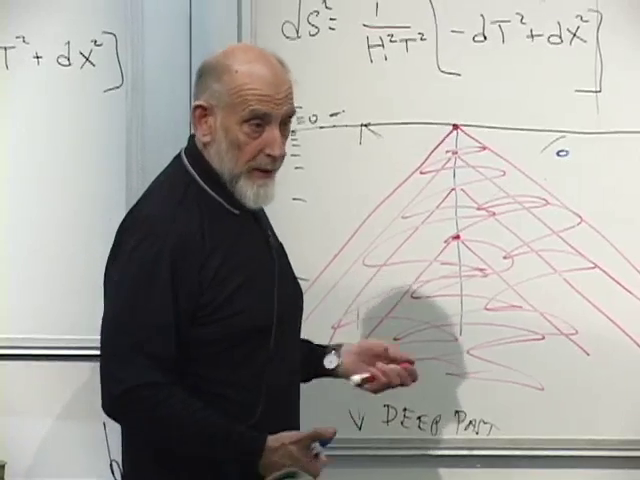
\includegraphics[width=0.88\textwidth]{lecture_08_figure_15.png}
\caption{Alice的极限过去光锥。其零边界是她依赖于观测者的德西特事件视界。}
\lectureframe{01:28:50.000}
\end{figure}

这个视界是私有的。不同的观测者有不同的未来端点，因而有不同的极限过去光锥。假设Bob曾经位于Alice的因果区域内，且两人交换过信息。如果Bob后来随哈勃流穿过Alice的视界，那么穿越之后发出的信号无法到达Alice，无论她等待多久。Bob有自己的视界，并最终失去接收Alice晚期信号的相应能力。

\begin{figure}[htbp]
\centering
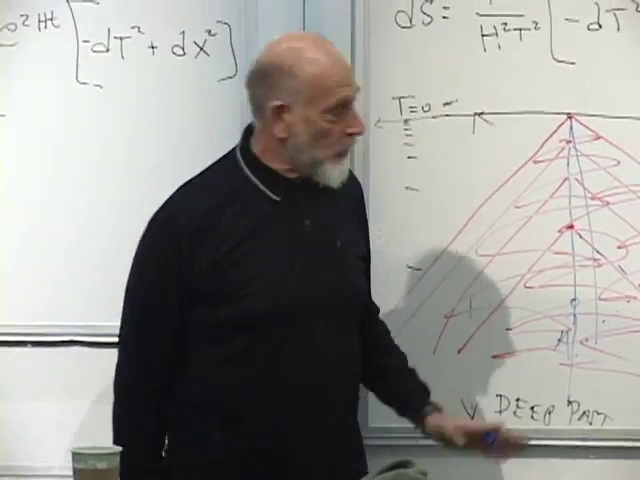
\includegraphics[width=0.88\textwidth]{lecture_08_figure_16.png}
\caption{Alice与Bob各有不同的因果边界。共动的Bob可以离开Alice的因果过去，尽管他们此前交换过信号。}
\lectureframe{01:30:20.000}
\end{figure}

如果Alice和Bob手拉手，或者更现实地说，保持在固定的固有间隔上束缚在一起，那么随着\(a^{-1}\)，他们的共动坐标间隔会缩小。在共形图中他们的曲线彼此靠近，但这并不意味着他们的固有距离消失。增长的共形因子补偿了缩小的坐标间隔，通信可以无限期地保持可能。

\begin{classroomqa}
\audiencequestion{在视界将他们分隔之后，Bob能同时看到Alice吗？\lecturetimestamp{01:31:43}}
\lecturerresponse{没有任何观测者会以那种字面意义同时看到一个遥远事件；观测总是对过去光锥中某个事件的观测。更准确的说法是，在穿越视界之后，来自另一条世界线的新发出的信号都无法到达。}
\end{classroomqa}

在远期宇宙学应用中，Alice代表我们束缚的局域残余，Bob代表每个未束缚的遥远星系。这些星系并不会在Alice时钟的某个有限时刻突然熄灭。它们后来的信号被拉伸到更长的时间间隔，并红移到更长的波长，直到在物理上变得不可探测。

\begin{classroomqa}
\audiencequestion{理论真的说在远期未来不会再有遥远的星系可见吗？\lecturetimestamp{01:33:38}}
\lecturerresponse{未束缚的星系越过局域观测者的事件视界。它们最后可见的信号变得越来越延迟、越来越红移，实际上只留下束缚的局域结构可观测。}
\end{classroomqa}

\section{视界处的红移}

仍然可以画出Bob发出的一个古老光信号在很晚的共形时刻到达Alice，这会使她看起来仍在看到他。物理内容在于这些信号的间隔和能量。Bob时钟的相等间隔到达时，被Alice固有时中越来越大的间隔所分隔。频率和光子能量下降：
\begin{equation}
\nu_{\rm received}\longrightarrow0,
\qquad
E_{\rm received}=h\nu_{\rm received}\longrightarrow0.
\end{equation}
Bob的影像变慢、变红并逐渐消失。极限信号携带的可利用信息趋于零。

\begin{figure}[htbp]
\centering
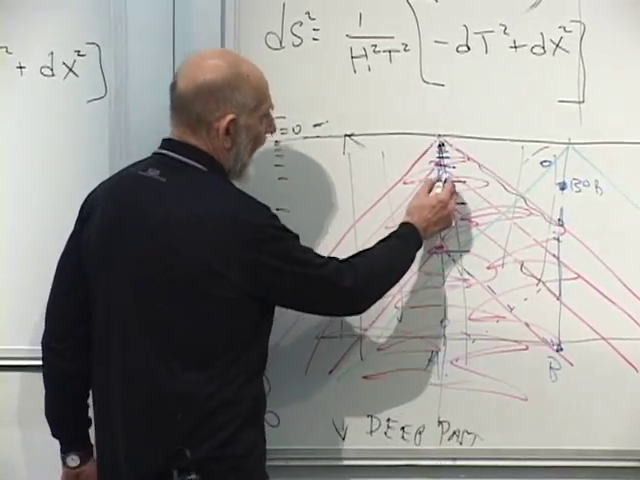
\includegraphics[width=0.89\textwidth]{lecture_08_figure_17.png}
\caption{比较德西特视界红移与熟悉的黑洞视界外部图像的后期板书状态。}
\lectureframe{01:36:20.000}
\end{figure}

\begin{classroomqa}
\audiencequestion{这像黑洞吗？在黑洞情形中，外部观测者永远看不到下落物体穿过视界。\lecturetimestamp{01:36:09}}
\lecturerresponse{是的。在两种情形中，观测者接收到的信号都越来越红移，并且从未直接看到穿越完成。因果图说明了哪些后来的发射永远无法到达；红移则解释了最后可观测的信息如何逐渐消失。}
\end{classroomqa}

这个类比引出了关于温度的问题。

\begin{classroomqa}
\audiencequestion{Alice如何能测量视界正上方的温度？\lecturetimestamp{01:39:34}}
\lecturerresponse{从操作上讲，她可以把温度计系在缆绳上放下去，使其不越过视界，然后再收回来。de Sitter观测者可以想象在宇宙学视界附近进行类似的实验。在量子理论中视界是热的，但本次讲座止步于经典几何，将那个计算推迟。}
\end{classroomqa}

这里没有推导de Sitter温度的公式。Hawking辐射只是作为对这一经典图像的量子修正的预告而出现。

\section{固定的视界半径}

共形图可以翻译回原来的时间坐标。两个共动点保持固定的坐标间隔，满足
\begin{equation}
D(t)=e^{Ht}\lvert\Delta x\rvert,
\end{equation}
因此它们的固有距离按指数增长。

\begin{classroomqa}
\audiencequestion{同样的运动在原来的、未变换的时间坐标中看起来是什么样子？\lecturetimestamp{01:41:14}}
\lecturerresponse{对于固定的共动坐标，整个空间度规随\(e^{2Ht}\)增长；因此固有间隔按\(e^{Ht}\)增长。撤销坐标变换就使这一膨胀变得明确。}
\end{classroomqa}

视界的行为不同，因为它与Alice之间的共动坐标距离并不固定。从终止于\(T=0\)的\(45^\circ\)零测地线来看，在恒定\(T<0\)的切片上视界距离为
\begin{equation}
\Delta x_H=-T=\frac{1}{H}e^{-Ht}.
\label{eq:l08-coordinate-horizon}
\end{equation}
乘以尺度因子得到
\begin{equation}
D_H(t)=a(t)\Delta x_H
=e^{Ht}\frac{e^{-Ht}}{H}
=\frac{1}{H}.
\label{eq:l08-fixed-horizon}
\end{equation}
恢复单位后，\(D_H=c/H\)。坐标间隔缩小，度规尺度增长，而它们的乘积保持不变。

\begin{classroomqa}
\audiencequestion{随着时间推移，从Alice到视界的距离是增长、缩小还是保持不变？\lecturetimestamp{01:42:42}}
\lecturerresponse{它保持不变。其坐标距离缩小，而共形因子增长，使得固有视界半径在\(c=1\)的单位下固定为\(H^{-1}\)。}
\end{classroomqa}

\begin{figure}[H]
\centering
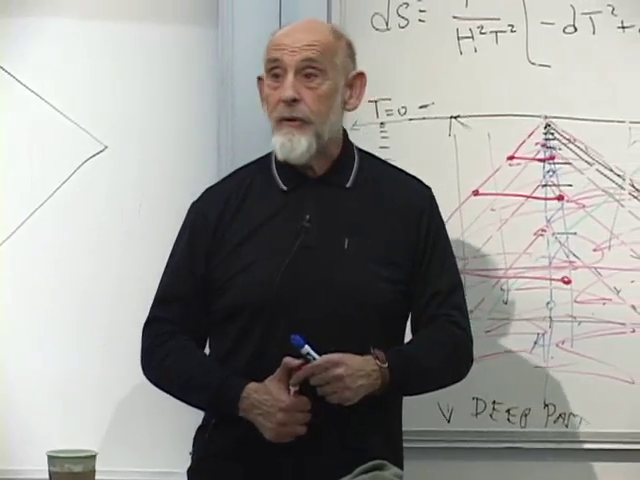
\includegraphics[width=0.90\textwidth]{lecture_08_figure_18.png}
\caption{最终的板书状态：相继的水平切片到视界的坐标距离不断缩小，但固有距离相同。}
\lectureframe{01:43:20.000}
\end{figure}

\begin{classroomqa}
\audiencequestion{Alice是否因为旧的图像从未完全消失而继续看到过去投影到视界上？\lecturetimestamp{01:43:45}}
\lecturerresponse{在经典上，这些图像只在极限意义上持续存在，即它们因无界红移而变得越来越难以探测。这一陈述忽略了与视界相关的Hawking辐射，它将修正量子描述。}
\end{classroomqa}

因此讲座在一个精确的边界处结束。真空能产生了指数膨胀；指数膨胀产生了一个固定的、依赖于观测者的事件视界；而该视界附近的信号已被驱动到趋于零的频率。视界的温度和Hawking辐射属于接下来的内容。正如Susskind所说，假设我们不会越过彼此的视界，我们将在下一讲再见。

\chapter{de Sitter 视界与宇宙学概率}

\lectureoverview{视界不仅仅是一个因果边界。对于静止观测者而言，它是一个热系统：在距视界固有距离 \(\rho\) 处放置的温度计读出的温度量级为 \(1/(2\pi\rho)\)，而引力红移使得远处看到的辐射要冷得多。我们将把这一黑洞的经验带入 de Sitter 空间，推导固定的视界半径 \(H^{-1}\)，并写出观测者的静态区度规。讲座的后半部分将追踪热力学的令人不安的后果：有限的 de Sitter 熵、Poincaré 回归、Boltzmann 大脑、永恒暴胀以及测度问题。最后的讨论将弦理论中精确的超对称结构与可能描述我们世界的、仍然未知的框架区分开来。}

\section{视界为何是热的}

我们在正式讲座之前开始，先提出决定今晚方向的问题。

\begin{classroomqa}
\audiencequestion{宇宙视界中并不包含黑洞。那么它究竟通过什么机制可以是热的？\lecturetimestamp{00:00:17}}
\lecturerresponse{机制与黑洞视界相同。有用的问题是操作性的：在视界附近放置的温度计记录到什么，以及什么样的辐射会到达远离视界的观测者？}
\end{classroomqa}

第一个实验是局部的。将温度计保持在距任意光滑、非极端视界的固定固有距离 \(\rho\) 处。足够靠近视界时，几何具有普适的 Rindler 形式，温度计读数为
\begin{equation}
T_{\rm local}(\rho)\simeq \frac{1}{2\pi\rho}
\label{eq:l09-local-temperature}
\end{equation}
其中采用 \(\hbar=c=k_B=1\) 的单位制。恢复常数后得到
\begin{equation}
k_B T_{\rm local}(\rho)\simeq \frac{\hbar c}{2\pi\rho}.
\end{equation}
当 \(\rho\to0\) 时的发散并不意味着下落观测者会遇到一个普通的物质火炉。它是由一位始终静止在视界外侧、因而必须越来越剧烈地加速的观测者所赋予的温度。

开场对话还区分了三个容易被混为一谈的概念：能量、温度和熵。

\begin{classroomqa}
\audiencequestion{如果把光子送入黑洞，我们测量的熵是否仍然相同，还是只有能量发生变化？\lecturetimestamp{00:01:22}}
\lecturerresponse{一旦光子变得不可及、位于视界之后，额外的信息就被隐藏了。在这里使用的简化比特语言中，一个光子可以隐藏一个额外的比特，从而增加熵。能量、温度和熵相互关联，但它们不可互换。}
\end{classroomqa}

\editorialnote{对于物理黑洞，熵变由 \(dS=dE/T_H\) 在热力学上确定；它并非对每个光子都普遍地为一个比特，而与能量无关。一比特的说法是讲座中的信息论理想化。}

近视界区域不断发射并重新吸收高频量子涨落。视界使这些涨落对静止观测者而言成为热性的。然而这立即引出一个谜题。如果该区域任意地热，为什么远处的观测者没有被任意高能的 photon 致盲？

\section{红移与 Hawking 温度}

普通的炽热墙壁即使我们站得很远，仍然是高频辐射的源。视界则不同，因为它的辐射必须爬过引力红移。光子的速度仍为 \(c\)；减小的是它的能量，
\begin{equation}
E=\hbar\omega,
\qquad
\omega_{\rm received}<\omega_{\rm emitted}.
\end{equation}
讲座中使用的粉笔类比仅在此点之前有用。抛出的石头上升时会减速，而光子继续以光速运动，同时其频率和能量减小。

对于 Schwarzschild 黑洞，无穷远处观测者测得的温度为
\begin{equation}
T_H=\frac{1}{8\pi M}
\label{eq:l09-hawking-natural}
\end{equation}
其中单位为 \(G_N=\hbar=c=k_B=1\)。在普通单位中，
\begin{equation}
T_H=\frac{\hbar c^3}{8\pi G_N M k_B}.
\label{eq:l09-hawking-full}
\end{equation}

\begin{figure}[htbp]
\centering
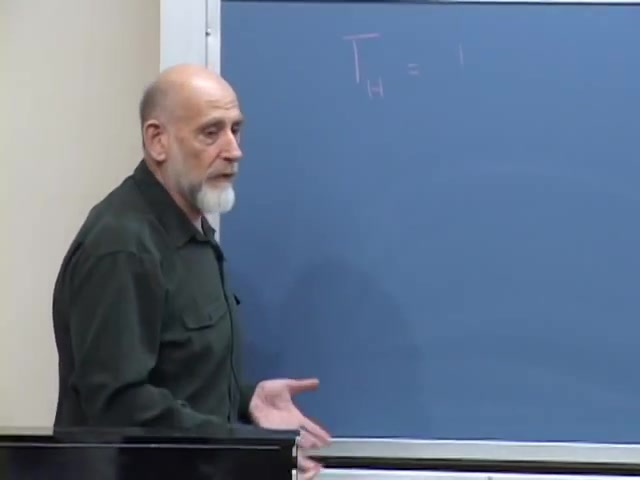
\includegraphics[width=0.68\textwidth]{lecture_09_figure_02.png}
\caption{自然单位下的 Hawking 温度 \(T_H=1/(8\pi M)\)。}
\lectureframe{00:08:12}
\end{figure}

更大的黑洞更冷。讲座通过追溯一个典型光子的反向路径来解释这一点。热光子具有特征能量 \(E_\gamma\sim T_H\)。一个以 \(M^{-1}\) 量级的能量到达无穷远的光子，当它从视界附近出发时具有大得多的局域能量。对于更大的黑洞，近视界层与无穷远之间的红移更为严重，从而留下更低的渐近温度。

\begin{classroomqa}
\audiencequestion{如果 Schwarzschild 时间在视界处冻结，我们是否应该追踪最初落入并构建了黑洞的那个光子？\lecturetimestamp{00:04:19}}
\lecturerresponse{对于温度问题，应追踪向外发射的光子。它们以非常高的局域频率出发，在向外爬升时损失能量，并作为 Hawking 辐射到达。最初下落光子的命运是一个独立的信息问题。}
\end{classroomqa}

\section{Planck 层与拉伸视界}

方程~\eqref{eq:l09-local-temperature}中的局域关系能在多大程度上被信任？本讲将普朗克长度视为半经典描述中有意义的最短距离。这提示存在一个薄层，大致位于数学视界之外一个普朗克长度处，其中充满普朗克尺度的涨落。它持续地发射和吸收。

大多数发射出的量子并不会逃逸。只有那些被导向一个非常狭窄的向外锥体内的量子才能避免落回。以一般角度发射的量子会返回视界。出射和入射的激发相互碰撞，产生粒子对和其他粒子；在这个意义上，定态描述包含一层极热物质的薄壳。

\begin{figure}[htbp]
\centering
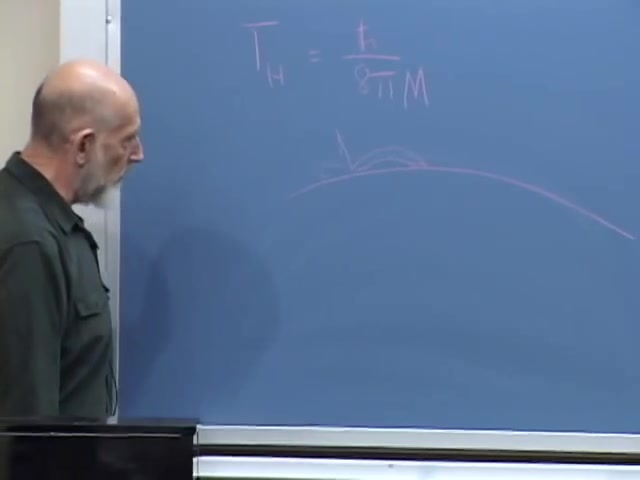
\includegraphics[width=0.74\textwidth]{lecture_09_figure_03.png}
\caption{近视界辐射的狭窄逃逸锥。大多数局域发射的量子返回视界。}
\lectureframe{00:11:38}
\end{figure}

存在一个互补的时空图像。远离视界时，一个虚涨落可以示意性地用一个短闭合圈表示：一个粒子-反粒子激发在能够成为渐近态之前就出现并消失。在视界附近，一个涨落可以跨越因果边界。对外部观察者而言，外侧部分看起来像是由视界发射、随后又被重新吸收的粒子。极小一部分逃逸并成为霍金辐射。

\begin{classroomqa}
\audiencequestion{在外部图中，这样的涨落是否从\(t=-\infty\)延伸到\(t=+\infty\)？\lecturetimestamp{00:15:00}}
\lecturerresponse{精确的经典视界导致那种看似奇异的描述。实际上我们用一个拉伸视界来代替它，即位于外部约一个普朗克长度处的一个类时曲面。于是发射和重新吸收在有限的外部时间中发生。}
\end{classroomqa}

\begin{figure}[htbp]
\centering
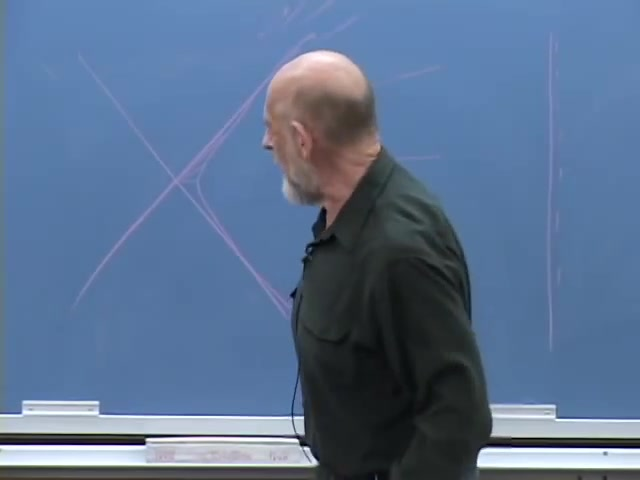
\includegraphics[width=0.72\textwidth]{lecture_09_figure_04.png}
\caption{经典视界以及外部描述中使用的邻近拉伸视界。}
\lectureframe{00:15:52}
\end{figure}

拉伸视界并不是一个新的不变边界。它是一个有效曲面，被放置在半经典几何不再可靠之处。物质以及几何本身的量子涨落将精确位置在普朗克尺度上抹平。这一构造将那种不确定性打包到一个曲面上，使得外部描述在该曲面上仍然有限。

在这个局域论证中，没有任何东西知道视界属于黑洞还是属于加速宇宙。这就是通往德西特空间的桥梁。

\section{膨胀坐标中的德西特空间}

正式讲授从德西特时空的空间平坦切片开始，
\begin{equation}
ds^2=-dt^2+e^{2Ht}d\mathbf{x}^2,
\qquad
d\mathbf{x}^2=dx^2+dy^2+dz^2.
\label{eq:l09-flat-slicing}
\end{equation}
常数\(H\)是德西特膨胀率。因子以\(e^{2Ht}\)的形式出现，是因为度规测量的是距离平方；一个固定的坐标间隔具有物理长度
\begin{equation}
D(t)=e^{Ht}\lvert\Delta\mathbf{x}\rvert.
\end{equation}

\begin{figure}[htbp]
\centering
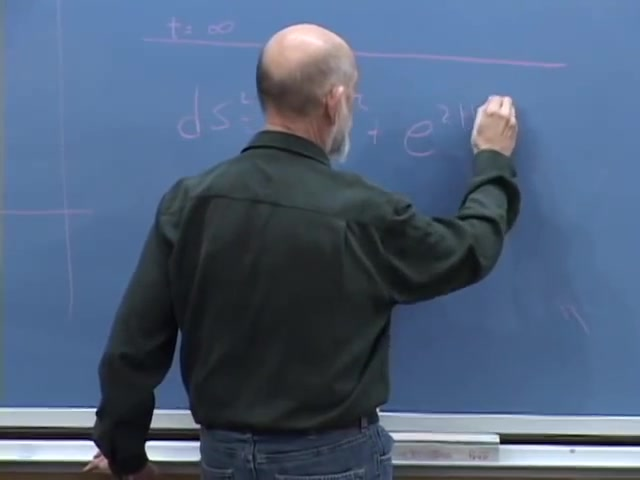
\includegraphics[width=0.78\textwidth]{lecture_09_figure_05.png}
\caption{平坦坐标中指数膨胀的德西特度规。}
\lectureframe{00:18:50}
\end{figure}

这些坐标使膨胀变得透明，但把未来无穷远放在图页上方无穷远处。为了把它带到黑板上，引入共形时间
\begin{equation}
\eta=-\frac{1}{H}e^{-Ht},
\qquad
-\infty<\eta<0.
\label{eq:l09-conformal-time}
\end{equation}
于是
\begin{equation}
dt=\frac{d\eta}{-H\eta},
\qquad
e^{Ht}=-\frac{1}{H\eta},
\end{equation}
而方程~\eqref{eq:l09-flat-slicing}变为
\begin{equation}
ds^2=\frac{1}{H^2\eta^2}
\left(-d\eta^2+d\mathbf{x}^2\right).
\label{eq:l09-conformal-metric}
\end{equation}
当\(t\to+\infty\)时，\(\eta\to0^{-}\)。无限固有时被压缩到有限水平线\(\eta=0\)。

\editorialnote{时间变换在黑板上书写时被修正了数次。方程~\eqref{eq:l09-conformal-time}是一致的形式：早期宇宙时间映射到\(\eta\to-\infty\)，而未来无穷远映射到\(\eta\to0^{-}\)。}

\begin{figure}[htbp]
\centering
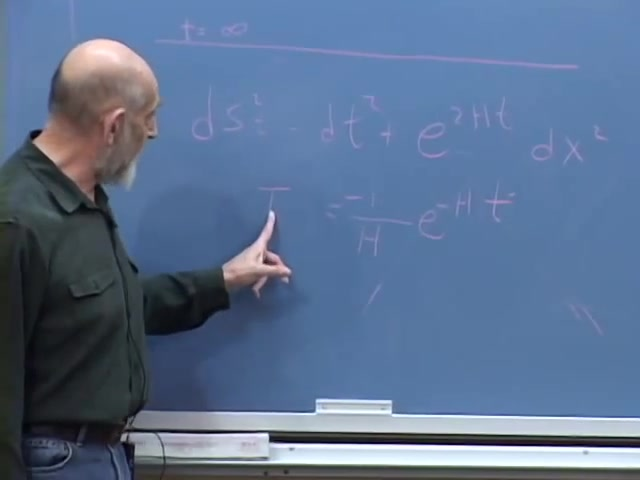
\includegraphics[width=0.82\textwidth]{lecture_09_figure_06.png}
\caption{共形时间变换以及共形平坦度规。}
\lectureframe{00:21:24}
\end{figure}

共形因子同时乘在时间项和空间项上，因此它不改变零方向。对于径向光线，
\begin{equation}
ds^2=0
\quad\Longrightarrow\quad
-d\eta^2+dx^2=0
\quad\Longrightarrow\quad
\frac{dx}{d\eta}=\pm1.
\label{eq:l09-null-rays}
\end{equation}
因此光在共形图中以\(45^\circ\)传播。这就是坐标变换有用的原因：因果可达性变得可见。

\section{一个观察者的因果片区}

想象一个观察者，其世界线延续无限固有时。在紧致化图上，它终止于\(\eta=0\)上的一个点。该观察者能够接收到的每一个信号都位于该终点的后向光锥之内。无论观察者等待多久，锥外的事件都永远无法与该观察者通信。

\begin{figure}[htbp]
\centering
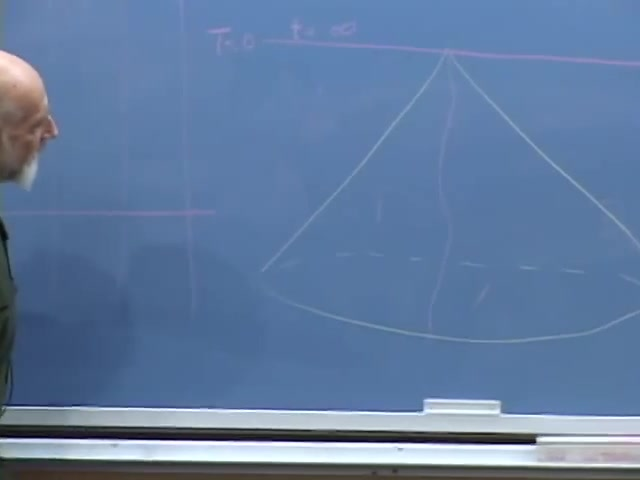
\includegraphics[width=0.78\textwidth]{lecture_09_figure_07.png}
\caption{共形德西特坐标中一个观察者的极限后向光锥。}
\lectureframe{00:24:38}
\end{figure}

第二个观察者有不同的锥。两个可及区域相互重叠，但二者都不是整个时空。在论证的剩余部分，我们采用第一个观察者的视角，并把那个后向光锥称为该观察者的因果片区。

这幅图似乎让这块区域朝未来收缩，但坐标宽度并不是固有距离。在\(\eta\)为常数的切片上，位于\(x=0\)的观测者与位于\(x=\Delta x\)的视界之间的固有距离平方为
\begin{equation}
D^2=\frac{(\Delta x)^2}{H^2\eta^2}.
\label{eq:l09-horizon-distance-start}
\end{equation}
视界是一条\(45^\circ\)的零线，终止于\(\eta=0\)，因此
\begin{equation}
\Delta x=\lvert\eta\rvert.
\end{equation}
代入后得到
\begin{equation}
D_{\rm hor}^2=\frac{1}{H^2},
\qquad
D_{\rm hor}=\frac{1}{H}.
\label{eq:l09-horizon-radius}
\end{equation}
坐标间隔在收缩，但共形因子恰好以补偿的量增长。固有视界半径是常数。

\begin{figure}[htbp]
\centering
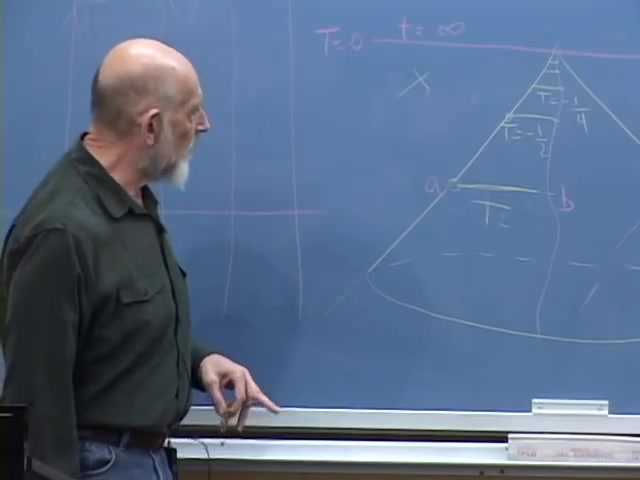
\includegraphics[width=0.80\textwidth]{lecture_09_figure_08.png}
\caption{将收缩的坐标间隔转换为固定固有距离\(H^{-1}\)的黑板推导。}
\lectureframe{00:28:42}
\end{figure}

\section{静态区域}

固定的视界半径提示我们采用适配中心观测者的坐标。讲座没有推导坐标变换，而是直接写出结果：
\begin{equation}
ds^2=
-\left(1-H^2r^2\right)d\tau^2
+\frac{dr^2}{1-H^2r^2}
+r^2d\Omega_2^2.
\label{eq:l09-static-patch}
\end{equation}
系数依赖于\(r\)，而不依赖于\(\tau\)。该图覆盖观测者的静态区域，
\begin{equation}
0\le r<\frac{1}{H}.
\end{equation}

\begin{figure}[htbp]
\centering
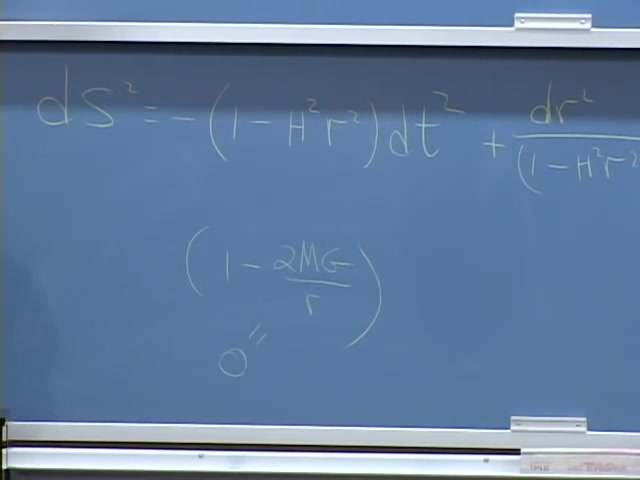
\includegraphics[width=0.88\textwidth]{lecture_09_figure_09.png}
\caption{de Sitter静态区域度规及其与Schwarzschild因子的比较。}
\lectureframe{00:34:22}
\end{figure}

与Schwarzschild的相似性立刻显现：
\begin{equation}
f_{\rm dS}(r)=1-H^2r^2,
\qquad
f_{\rm Schw}(r)=1-\frac{2G_NM}{r}.
\end{equation}
在两种情形中，静态坐标下的视界都出现在\(f(r)=0\)处。对于de Sitter，
\begin{equation}
1-H^2r^2=0
\quad\Longrightarrow\quad
r_H=H^{-1}.
\end{equation}
该图在那里是奇异的，正如Schwarzschild坐标在黑洞视界处奇异一样。然而，整体几何在一个重要方面有所不同。黑洞观测者站在外面向内看；de Sitter观测者站在里面向外看。

\begin{classroomqa}
\audiencequestion{在一个指数膨胀的宇宙中，自由释放的粒子彼此远离，几何怎么可能是静态的？\lecturetimestamp{00:36:06}}
\lecturerresponse{静态并不意味着每个粒子都保持不动。它意味着度规系数以及重复实验的结果与起始时间无关。现在释放两个粒子，它们会加速分离；稍后重复同样的实验，同样的运动仍会发生。}
\end{classroomqa}

\begin{classroomqa}
\audiencequestion{这两个分离的粒子会看到彼此红移吗？\lecturetimestamp{00:38:34}}
\lecturerresponse{会。尽管适配观测者的度规与时间无关，它们不断增大的间距仍会产生相对红移。}
\end{classroomqa}

\section{从内部看到的温度}

Schwarzschild空间与de Sitter空间的近视界结构是局部等价的。因此，de Sitter视界会发射并重新吸收热量子。一个稀有的光子向内传播到中心观测者，在爬升静态区域的势时损失能量。中心测得的Gibbons--Hawking温度为
\begin{equation}
T_{\rm dS}=\frac{H}{2\pi}
\label{eq:l09-de-sitter-temperature}
\end{equation}
（自然单位制）。位于半径\(r\)处的静止温度计读数为Tolman红移后的值
\begin{equation}
T_{\rm local}(r)=
\frac{T_{\rm dS}}{\sqrt{1-H^2r^2}},
\label{eq:l09-tolman}
\end{equation}
当\(r\to H^{-1}\)时它发散，而在视界附近约化为式~\eqref{eq:l09-local-temperature}。

\editorialnote{讲座从视界距离和红移得到标度，而没有明确写出式~\eqref{eq:l09-de-sitter-temperature}和\eqref{eq:l09-tolman}。它们陈述了该论证的标准归一化。}

对于观测到的晚期加速，讲座使用周期估计
\begin{equation}
H^{-1}\sim 20\times10^9\ {\rm light\ years}.
\label{eq:l09-lecture-horizon-estimate}
\end{equation}
于是，一个典型的视界光子具有与数十亿光年相当的波长。这不是微波背景辐射；它要冷得多。

操作性的思想实验是一根宇宙尺度的钓鱼竿。Alice留在\(r=0\)处，把温度计系在一根同时能传输数据的极长线上，并让宇宙排斥把仪器带向外面。她在刚好不到视界处让它停下，等待信号返回，发现局域温度很高。她身旁位于中心的温度计则读出微小的值\(H/(2\pi)\)。同一个视界支持这两种读数，因为它们是在不同的引力势处测得的。

\section{穿越视界}

经典的从外部进行的描述类似于人们熟悉的黑洞故事。位于中心的Bob看着Alice远去。她的信号红移越来越强，到达得越来越慢；她看起来被压扁在视界上，并最终消失。后来的旅行者Jane则表现为边界附近沉积层中的又一层更薄的层。

\begin{classroomqa}
\audiencequestion{从我们的观点看，物体究竟会穿过宇宙视界吗？\lecturetimestamp{00:45:30}}
\lecturerresponse{在静态观测者的经典描述中不会。它们的信号红移并消失，而它们的表观位置趋近视界。然而，在它们自身自由下落的描述中，它们会穿过视界，而不会遇到局部奇异的表面。}
\end{classroomqa}

\begin{classroomqa}
\audiencequestion{视界只对始终留在近旁而不穿越的观测者才是热的吗？自由下落的观测者并不会仅仅因为穿过视界就被烤熟，对吧？\lecturetimestamp{00:48:27}}
\lecturerresponse{艾丽丝在她自己的参考系中平滑地穿过。极端温度属于静止描述。如果鲍勃坚持要把艾丽丝分辨得越来越靠近视界，他就必须用越来越短的波长去照射她。于是，这个尝试中的海森堡显微镜所沉积的能量足以烤熟它试图观测的对象。}
\end{classroomqa}

这并不是两个局域事件之间的矛盾。静止观测者和自由下落者使用的是截然不同的测量。视界互补性所问的是：如何才能使这两种描述都成立，而又不允许一个观测者直接比较重复的信息。

\section{真空排斥的牛顿模型}

此时有学生问，什么取代了黑洞的引力势阱。萨斯坎德通过构造一个牛顿模型来回答。设 \(\phi\) 为引力势，则检验粒子的加速度为
\begin{equation}
\mathbf{a}=-\boldsymbol{\nabla}\phi.
\end{equation}
对于普通的非相对论物质，泊松方程为
\begin{equation}
\nabla^2\phi=4\pi G_N\rho.
\label{eq:l09-poisson}
\end{equation}

\begin{classroomqa}
\audiencequestion{如果黑洞效应来自其引力势阱，那么在德西特空间中相应的源是什么？\lecturetimestamp{00:49:36}}
\lecturerresponse{真空能量本身提供了一个空间上均匀的引力源。在牛顿描述中，它产生的是二次势，而不是 \(1/r\) 势阱。}
\end{classroomqa}

\begin{figure}[htbp]
\centering
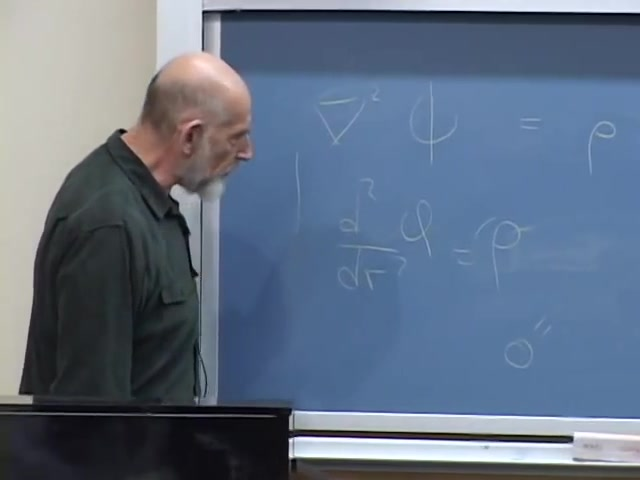
\includegraphics[width=0.78\textwidth]{lecture_09_figure_10.png}
\caption{泊松方程与讲义中示意性的径向二阶导数形式。}
\lectureframe{00:51:38}
\end{figure}

黑板上省略了归一化、球面测度项、压强，起初甚至省略了整体符号，把这个练习简化为
\begin{equation}
\frac{d^2\phi}{dr^2}\sim H^2.
\end{equation}
关键的推断是：常数源给出二次函数。取德西特排斥所需的符号，
\begin{equation}
\phi_{\rm dS}(r)=-\frac{1}{2}H^2r^2,
\qquad
a_r=-\frac{d\phi_{\rm dS}}{dr}=H^2r.
\label{eq:l09-de-sitter-potential}
\end{equation}
加速度指向外侧，并随距离线性增长。解 \(\ddot r=H^2r\) 得到
\begin{equation}
r(\tau)=A e^{H\tau}+B e^{-H\tau},
\end{equation}
因此增长分支再现了指数分离。

\begin{figure}[htbp]
\centering
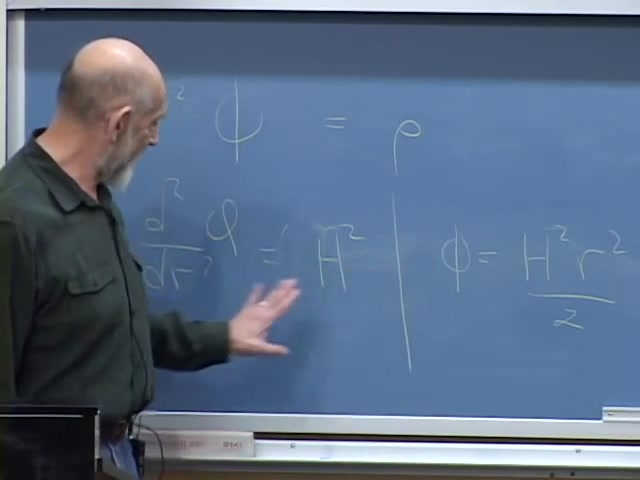
\includegraphics[width=0.76\textwidth]{lecture_09_figure_11.png}
\caption{均匀源方程与二次德西特势。}
\lectureframe{00:53:32}
\end{figure}

\editorialnote{在广义相对论中，均匀流体的弱场加速度取决于 \(\rho+3p\)，而不只是 \(\rho\)。真空能量有 \(p=-\rho\)，所以 \(\rho+3p=-2\rho\)，加速度是排斥性的。式~\eqref{eq:l09-de-sitter-potential} 是正确归一化的德西特结果；黑板上的计算有意只追踪二次依赖关系和符号。}

在中心放置一个普通质量 \(M\)。定性势变为
\begin{equation}
\phi(r)=-\frac{G_NM}{r}-\frac{1}{2}H^2r^2,
\label{eq:l09-combined-potential}
\end{equation}
径向加速度为
\begin{equation}
a_r=-\frac{G_NM}{r^2}+H^2r.
\end{equation}
在小 \(r\) 处，局域吸引占优；在大 \(r\) 处，真空排斥占优。二者的平衡发生在
\begin{equation}
r_\ast=\left(\frac{G_NM}{H^2}\right)^{1/3}.
\label{eq:l09-turnaround}
\end{equation}
这就是讲义中势极大值的干净版本。它定性地解释了为什么邻近的引力束缚系统能够保持在一起，而足够遥远的星系则在加速远离。

\begin{figure}[htbp]
\centering
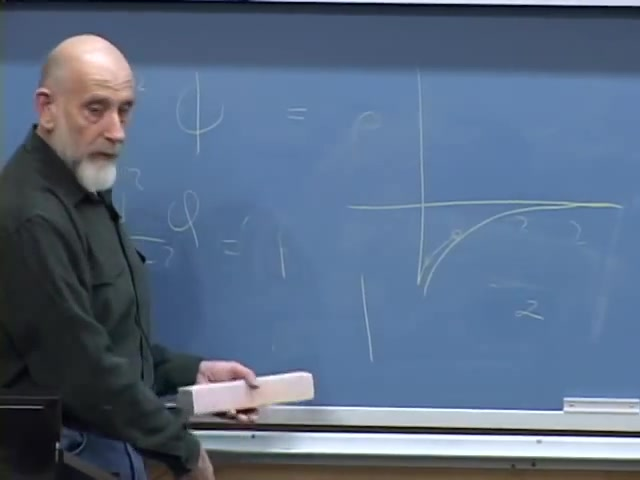
\includegraphics[width=0.78\textwidth]{lecture_09_figure_12.png}
\caption{普通 \(1/r\) 吸引与倒置的二次德西特势相结合。}
\lectureframe{00:58:20}
\end{figure}

\begin{classroomqa}
\audiencequestion{普通力仍然重要吗，还是真空排斥最终会撕碎每一个物质岛屿？\lecturetimestamp{00:57:29}}
\lecturerresponse{必须包括所有力。在足够小的尺度上，电磁束缚和局域引力占主导。真空排斥只有在由 \(H^{-1}\) 以及适合该束缚质量的平衡尺度所设定的巨大距离上才变得重要。}
\end{classroomqa}

\section{一个源，几个名称}

讨论现在在术语上稍作停顿。在所采用的模型中，真空能量、宇宙学常数和暗能量并不是三种相加的物质。它们是同一个 \(w=-1\) 源的三种描述。人们可以谈论爱因斯坦方程中的常数项、真空的洛伦兹不变能量密度，或者驱动晚期加速的分量。

\begin{classroomqa}
\audiencequestion{均匀牛顿源和量子真空能量是否作为两种独立的效应同时存在？\lecturetimestamp{00:59:14}}
\lecturerresponse{不。均匀密度是同一个源的牛顿模型。真空能量、宇宙学常数，以及本讲中的暗能量，指的是同一个物理分量。}
\end{classroomqa}

\begin{classroomqa}
\audiencequestion{那么，同一现象是否既有经典描述又有量子描述？\lecturetimestamp{01:00:32}}
\lecturerresponse{它的微观起源可能是量子力学的，正如电子质量的一部分具有量子起源。一旦有效能量密度已知，它就作为普通源进入经典引力方程。我们并不知道所观测到的值的最终起源。}
\end{classroomqa}

在普朗克单位制中，观测到的真空能量密度极其微小，
\begin{equation}
\rho_\Lambda\sim10^{-123}\rho_{\rm Pl},
\label{eq:l09-planck-smallness}
\end{equation}
这取决于普朗克密度所采用的约定。这个微小的数值就是宇宙学常数问题。这也是视界如此之大的原因：在四维中，
\begin{equation}
H^2=\frac{8\pi G_N}{3}\rho_\Lambda,
\qquad
r_H=H^{-1}.
\end{equation}
如果\(H\)更大，视界就会更小，中心的德西特温度就会更高，排斥性加速度\(H^2r\)就会更强。

\begin{classroomqa}
\audiencequestion{微小的宇宙学常数是否与普朗克常数和量子涨落有关？\lecturetimestamp{01:03:27}}
\lecturerresponse{最清晰的比较使用无量纲的普朗克单位，其中\(G_N=\hbar=c=1\)。在这些单位下，真空密度比自然的普朗克密度低约\(123\)个数量级。解释这一层级结构是基础物理学的核心谜题之一。}
\end{classroomqa}

\begin{classroomqa}
\audiencequestion{真空能量必须是一个严格恒定的宇宙学常数吗？加速组分能否减小并最终趋于零？\lecturetimestamp{01:04:52}}
\lecturerresponse{这在逻辑上是一种可能的替代方案：一个动力学暗能量场可以随时间变化。本讲采用恒定情形，是因为当时可获得的观测越来越倾向于接近宇宙学常数的行为，而不是因为所有替代方案都已被证明不可能。}
\end{classroomqa}

\section{遥远未来的天文学}

在渐近德西特宇宙中，不受引力束缚的结构最终会越过观测者的视界。宇宙微波背景红移到可探测性以下。遥远的星系消失。一位幸存的天文学家可能只看到在一个原本黑暗的区域中一个并合后的局域引力岛。

\begin{classroomqa}
\audiencequestion{没有望远镜，会有人注意到遥远的星系已经消失了吗？\lecturetimestamp{01:06:17}}
\lecturerresponse{大概不会。严重的问题更为深刻：即使拥有先进的仪器，未来的观测者也可能缺乏我们今天借以推断膨胀的遥远示踪物和微波背景。}
\end{classroomqa}

那时，古老的岛宇宙图景可能显得很有说服力。奥伯斯佯谬不会迫使得出不同的结论，因为它假设了无限、静态、均匀的发光源分布；未来的观测者只会看到局域岛中有限的恒星。暗能量并不会不断从空无一物的空间中制造出替代星系。

精确德西特空间中的视界并不会围绕局域星系收缩。它的物理半径保持为\(H^{-1}\)，远大于一个星系。消失的是被带过那个固定因果边界的非束缚物质。

\begin{classroomqa}
\audiencequestion{从星系中抛射出的恒星能否作为检验天体来探测大尺度几何？\lecturetimestamp{01:11:25}}
\lecturerresponse{在一段时间内可以。被抛射的物体和长基线光信号可以探测几何。但只有当距离达到十亿光年的相当一部分量级时，效应才变得显著，因此该实验将需要宇宙学时间尺度。}
\end{classroomqa}

\begin{classroomqa}
\audiencequestion{我们怎么知道一个遥远的视界还没有把宇宙的大部分对我们隐藏起来？\lecturetimestamp{01:11:45}}
\lecturerresponse{我们已经看到足够多的星系、红移和背景辐射，足以测量膨胀并重建大尺度几何。被剥夺了这些示踪物的未来观测者将面临困难得多的推断问题。}
\end{classroomqa}

\begin{classroomqa}
\audiencequestion{如果视界恰好位于仙女座星系之外，它的存在会显而易见吗？\lecturetimestamp{01:12:19}}
\lecturerresponse{会。如此小的视界将要求大得多的\(H\)，由此产生的排斥将强烈改变仙女座星系（Andromeda）的运动。而测量值反而把渐近视界置于一个大得多的尺度上。}
\end{classroomqa}

\begin{classroomqa}
\audiencequestion{在我们的视界之外，是否可能正在发生新的大爆炸？\lecturetimestamp{01:13:25}}
\lecturerresponse{视界之外的事件对我们或我们的后代都不可见。一个相关但更精确的可能性，即永恒暴胀中的气泡成核，将在本讲后面介绍。}
\end{classroomqa}

借助火箭、时钟以及数十亿年的时间，未来的观测者可以派遣探索者穿越这片区域的大部分，并重建其度规。然而，在普通的实验室或文明时间尺度上，这一效应几乎无法触及。这一区分纠正了那个过强的断言，即膨胀将不可能被发现：它在操作上遥不可及，但并非原则上被禁止。

\begin{classroomqa}
\audiencequestion{未来的探索者能否比等待热复现更早得多地确定几何？\lecturetimestamp{01:21:40}}
\lecturerresponse{当然可以。复现并不是所提议的测量。探索者在数十亿光年的基线上交换光信号，可以在短得多、但仍属宇宙学的时间尺度上绘制静态区域。}
\end{classroomqa}

\begin{classroomqa}
\audiencequestion{红移会抹去这类探索者返回的所有信息吗？\lecturetimestamp{01:23:24}}
\lecturerresponse{如果他们在远处于视界内部的尺度上探测，就不会。约十亿光年的基线已经对膨胀敏感，同时只产生适度的红移。该实验主要受限于其极其漫长的持续时间。}
\end{classroomqa}

\section{有限熵与复现}

静态区域在热力学意义上并非空无一物。其视界具有面积
\begin{equation}
A_H=4\pi H^{-2},
\end{equation}
温度 \(T_{\rm dS}=H/(2\pi)\)，以及熵
\begin{equation}
S_{\rm dS}=\frac{A_H}{4G_N}
=\frac{\pi}{G_NH^2}
\label{eq:l09-de-sitter-entropy}
\end{equation}
单位为 \(\hbar=c=k_B=1\)。该熵是有限的。因此，人们可以谨慎地将静态区域描绘为一个有限熵的热腔，在稳态描述中其激发集中在视界附近。

处于平衡态的普通气体盒子在短时间尺度上看起来毫无特征，但统计力学并不禁止涨落。如果一个宏观态相对于平衡态具有熵亏 \(\Delta S\)，其概率大致为
\begin{equation}
P\sim e^{-\Delta S}.
\label{eq:l09-fluctuation-probability}
\end{equation}
相应的等待时间按如下方式增长
\begin{equation}
t\sim t_0 e^{\Delta S}.
\end{equation}
对于有限系统，重新访问一个任意接近先前状态的状态所需的时间就是庞加莱复现时间，
\begin{equation}
t_{\rm rec}\sim H^{-1}e^{S_{\rm dS}}.
\label{eq:l09-recurrence}
\end{equation}
由于我们视界的 \(S_{\rm dS}\) 约为 \(10^{120}\) 量级，讲座将该尺度概括为 \(e^{10^{120}}\)。前因子是以年、哈勃时间还是微观单位来衡量，与双指数相比都无关紧要。

\begin{figure}[htbp]
\centering
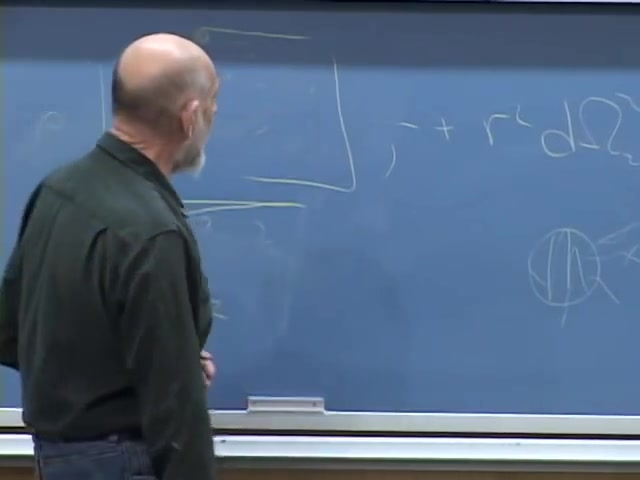
\includegraphics[width=0.76\textwidth]{lecture_09_figure_13.png}
\caption{关于复现的讨论，黑板上写着巨大的指数等待时间尺度。}
\lectureframe{01:16:24}
\end{figure}

在这样的复现之前，较小的涨落要常见得多。房间里的分子可能全部聚集在一个角落；一个复杂的涡旋可能短暂形成；在讲座诙谐的层级中，热运动可能组装出一头大象。所需的熵亏越小，涨落的代价就越低。

\begin{classroomqa}
\audiencequestion{庞加莱复现是否特指量子力学的结果？\lecturetimestamp{01:25:44}}
\lecturerresponse{不是。复现和稀有涨落已经在经典统计力学中出现。将它们应用于德西特空间使用的是我们目前的物理框架，这一框架有朝一日可能被修正，但热力学和统计推理是我们所知最稳固的结构之一。}
\end{classroomqa}

概率本身的含义可能在未来理论中加深。萨斯坎德并未声称相反。他更狭义的观点是，仅仅因为统计力学的长期含义显得奇怪就抛弃它，将丢弃物理学中经过最充分检验的组织原则之一。

\section{玻尔兹曼大脑与典型观测者}

假设一次热涨落创造出一个完整的类大爆炸状态。那需要巨大的熵减少。产生一个太阳系的涨落代价更低；一个已经温暖的 Earth 代价还要更低。如果唯一的要求是一个观测者，那么代价最低的涨落可能只创造出一个功能完备的大脑，并带有看似真实的记忆。这样一个假想的观测者被称为玻尔兹曼大脑。

问题不在于某一次奇异的涨落在逻辑上是否可能。而在于一个宇宙学模型是否预言几乎每一个观测者都是这样的涨落。我们从观测出发进行推理时，假设我们并非极其非典型。如果一个理论中具有连贯宇宙历史的普通观测者被孤立的熱大脑以指数方式超过，那就削弱了这一推断。

因此，玻尔兹曼大脑问题命名了一个定量一致性检验。人们将普通观测者的预期丰度与涨落产生的观测者的丰度进行比较。如果后者占主导，那么要么真空必须在它们增殖之前衰变，要么必须改变测度，要么必须重新考虑宇宙学假设。

先前关于紫外--红外联系的问题被明确推迟。复现论证并不依赖于解决那个单独的问题。

\section{永恒暴胀与气泡宇宙}

接下来，讲座在不试图给出完整推导的情况下引入第二个概率问题。一个亚稳态的德西特真空可以成核出一个气泡，其中真空能更低。气泡壁不断膨胀，其内部可以演化成一个开放的弗里德曼--罗伯逊--沃克宇宙。与此同时，周围暴胀的区域继续膨胀并成核出更多的气泡。

\begin{figure}[htbp]
\centering
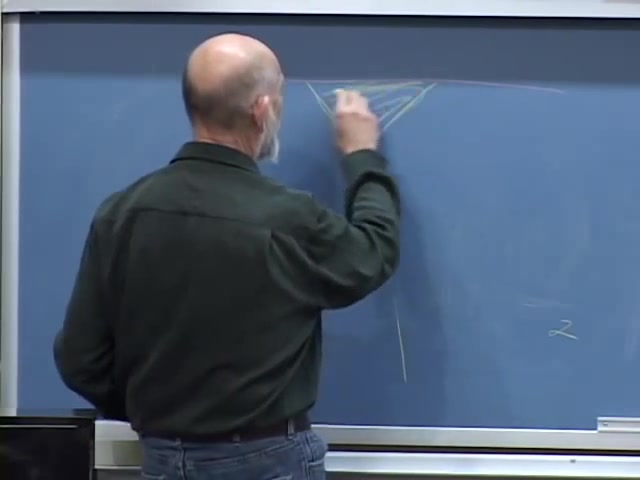
\includegraphics[width=0.74\textwidth]{lecture_09_figure_14.png}
\caption{一个真空能较低的气泡被画在暴胀的德西特背景之中。}
\lectureframe{01:29:38}
\end{figure}

关键特征是种群的指数增长。新物理体积产生的速度比气泡移除它的速度更快，因此气泡区域的数目无界增长。不同的气泡可能落入不同的低能态，从而表现出不同的有效物理。

为了揭示其中的统计困难，萨斯坎德首先离开宇宙学，考虑一个以指数增长、资源有限但未知的人类种群。假设观测者在所有曾经生活过的人中是典型的。如果种群每一代翻一番然后终结，那么一半的人生活在最后一代，四分之三生活在最后两代，八分之七生活在最后三代：
\begin{equation}
f_n=1-2^{-n}.
\label{eq:l09-last-generations}
\end{equation}
典型性于是会把我们置于令人不安地接近终结的位置，尽管我们对资源总量一无所知。这并不是作为对人类灭绝的可靠预言而提出的。它是一个警告：指数增长使得计数被截断所主导。

抛硬币的例子更清晰地陈述了通常的典型性假设。如果许多实验者每人抛一枚公平的硬币\(N\)次，绝大多数人会得到
\begin{equation}
n_H=\frac{N}{2}+O(\sqrt{N}).
\end{equation}
一个极端的观测者应当首先怀疑模型有误或硬币有问题，而不是在没有证据的情况下假定自己处于一个极其罕见的尾部。宇宙学概率使用同样的典型性直觉，但在无限种群中，它需要一种定义良好的计数方式。

\section{埃舍尔的边界与测度问题}

萨斯坎德的几何类比是M.\ C.\ 埃舍尔的\emph{圆极限IV}，即那个由天使与魔鬼铺满、越靠近边界显得越小的圆盘。在图画所表示的双曲几何中，这些图形是等价的；它们表观的欧几里得大小发生变化，仅仅是由于投影。

\begin{figure}[htbp]
\centering
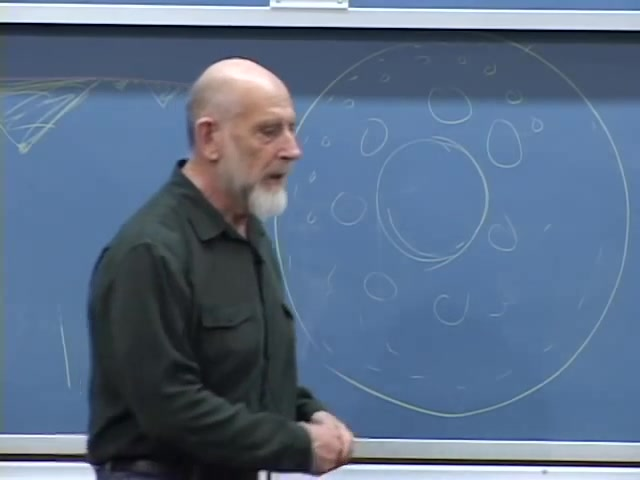
\includegraphics[width=0.76\textwidth]{lecture_09_figure_15.png}
\caption{埃舍尔在圆形边界附近指数增殖的图形在黑板上的替代物。}
\lectureframe{01:37:54}
\end{figure}

设想埃舍尔只有有限的时间、墨水和耐心。在边缘附近他最终会停下来，也许留下一些未完成的图形。由于图形数目随双曲半径指数增长，一个有限的外层包含所画每一个图形的一个固定比例。无论把截断向外移动多远，大致一半都可以位于最后一层中。

现在问天使与魔鬼之比。在理想的无限图案中，对称性暗示二者一一相等。然而在任何有限的计数中，一个稍有不同的边界都可能包含多得多的某一类图形。由于计数的大部分位于边界附近，该边界的微小形变就会使答案产生量级为一的变化。

\begin{figure}[htbp]
\centering
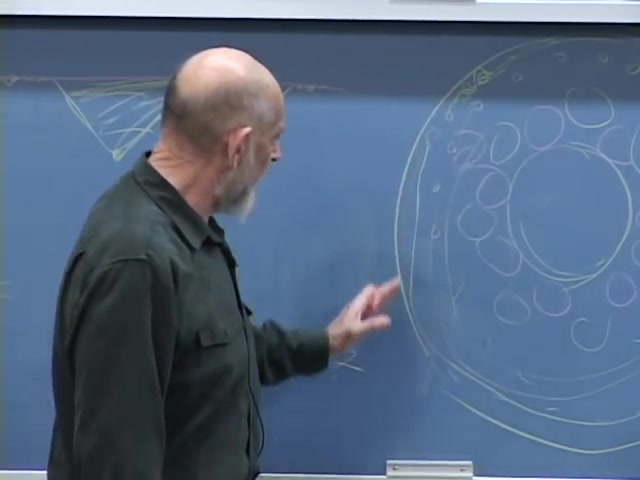
\includegraphics[width=0.76\textwidth]{lecture_09_figure_16.png}
\caption{在指数增长的图案中，截断边界主导着计数。}
\lectureframe{01:43:06}
\end{figure}

同样的模糊性出现在永恒暴胀中。数出某个时间截断以下的蓝色和粉色气泡宇宙，然后把截断推后。两种计数都发散，而它们的比值可能敏感地依赖于\emph{时间}意味着什么以及截断曲面如何画出。概率测度是一种对无限种群进行正规化并提取相对概率的规定。不同的看似合理的规定无法彼此一致，这就是测度问题。

\begin{classroomqa}
\audiencequestion{这个截断问题与重整化之间有关系吗？\lecturetimestamp{01:45:43}}
\lecturerresponse{有一个类比。在量子场论中，人们引入点阵或紫外截断，将其细化，并寻求对正规化子边缘细节不敏感的物理量。宇宙学家希望从永恒暴胀中得到同样稳健的提取，但在本文所讨论的框架中，目前还没有同样决定性的规定可用。}
\end{classroomqa}

这个类比不应被夸大。当受控的流确定出与正规化子无关的可观测量时，重整化才成功。测度问题恰恰在于，类似的不变量问题和取极限的程序仍然不清楚。说我们也许问错了问题，在给出正确的问题之前并不是一个解决方案。

\begin{classroomqa}
\audiencequestion{这个气泡图像与早期宇宙中的暴胀是同一种现象吗？\lecturetimestamp{01:48:19}}
\lecturerresponse{二者密切相关。在永恒暴胀中，母背景继续暴胀，而局部气泡内部则经历各自的宇宙学演化。我们的可观测宇宙可能位于这样一个区域之内。}
\end{classroomqa}

\section{气泡碰撞能被观测到吗？}

两个气泡相遇时，并不是简单地把它们的真空能相加。一个畴壁将真空态不同的区域分隔开来，而畴壁的几何形状决定了任一侧能够观测到什么。取决于碰撞相对于我们过去光锥的位置，其印记可能被隐藏，也可能可见。

\begin{classroomqa}
\audiencequestion{两个真空气泡碰撞时会发生什么？\lecturetimestamp{01:52:07}}
\lecturerresponse{碰撞会产生一种畴壁几何，其行为取决于两个真空以及壁的张力。在有利的因果条件下，这种扰动可以进入我们的可观测区域，并留下各向异性的印记。}
\end{classroomqa}

讲座讨论了宇宙微波背景中的一个冷斑区域作为可能的候选，并指出圆形特征周围的偏振可作为判别依据。这是有意作为一种可能性提出的，而非一项探测结果。一个有说服力的碰撞印记将是革命性的，因为它将为邻近气泡区域提供直接证据，并使测度问题在实验上变得紧迫。

\begin{figure}[htbp]
\centering
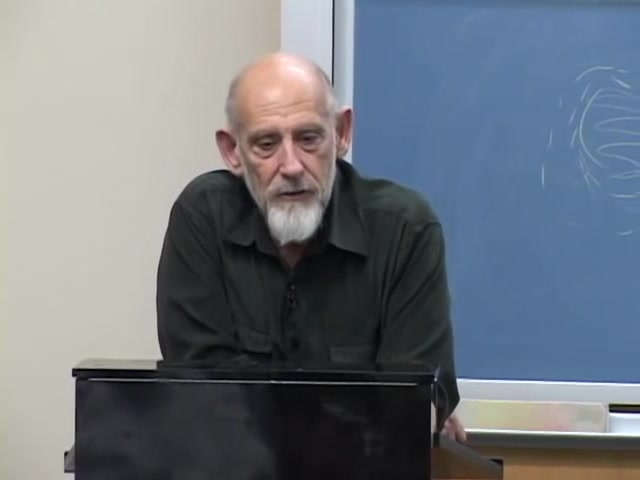
\includegraphics[width=0.70\textwidth]{lecture_09_figure_17.png}
\caption{气泡碰撞讨论中的圆形天空特征及其可能的偏振图样。}
\lectureframe{01:50:22}
\end{figure}

\editorialnote{冷斑的讨论记录了讲座当时的观测状况和提议。仅凭一个温度异常并不构成气泡碰撞的证据；还需要一个详细的、相互关联的印记。}

\begin{classroomqa}
\audiencequestion{这些气泡是四维的吗？其内部具有什么样的空间曲率？\lecturetimestamp{01:53:37}}
\lecturerresponse{它们是时空区域，而不是在外部时间中演化的三维肥皂泡。其内部通常是具有负空间曲率的开放FRW宇宙。碰撞会扰动该几何，但并不会简单地把负曲率变成正曲率。}
\end{classroomqa}

\section{弦理论确立了与未确立什么}

最后的讨论以邀请听众为弦理论正确赋予一个概率开始。Susskind拒绝给出这个数字，因为该命题过于含糊。他转而区分两个主张。

第一，存在一个高度受约束的、结合了量子力学与引力的数学结构。它产生了精确的结果和深刻的数学恒等式，其内部自洽性经受住了广泛的审视。用讲座中的非正式说法，这就是大写的\emph{String Theory}，即\(S\)。被理解得最清晰的那些版本严重依赖于超对称。

第二，观测到的世界在可及能量上并不是超对称的。要把精确的超对称构造与我们这个非超对称的宇宙联系起来，需要超对称破缺以及一个无法以同等精度加以控制的更大框架。用讲座中的说法，那个被寄予希望的扩展就是小写的\emph{string theory}，即\(s\)。

\begin{classroomqa}
\audiencequestion{人们能否为弦理论是自然的正确理论赋予一个概率？\lecturetimestamp{01:54:18}}
\lecturerresponse{如果不指明指的是哪一个主张，就无法负责任地做到。精确的数学结构确实存在，并且包含量子引力，但严格受控的超对称模型并不是字面意义上的我们所观测到的世界。一个更大的扩展是否包含我们的世界，是物理学家可以持有有根据的偏见的问题，而不是一个定义明确的数值概率。}
\end{classroomqa}

这里可以类比于完整数学工具尚未出现之前的力学。人们可能知道\(F=ma\)和平方反比力，却只能求解高度对称的圆轨道。可求解的部分会是真实的，但并不是整个理论。同样，精确的超对称弦构造可能只是一个更大结构中的一个特殊的、异常易于处理的区域。

\begin{figure}[htbp]
\centering
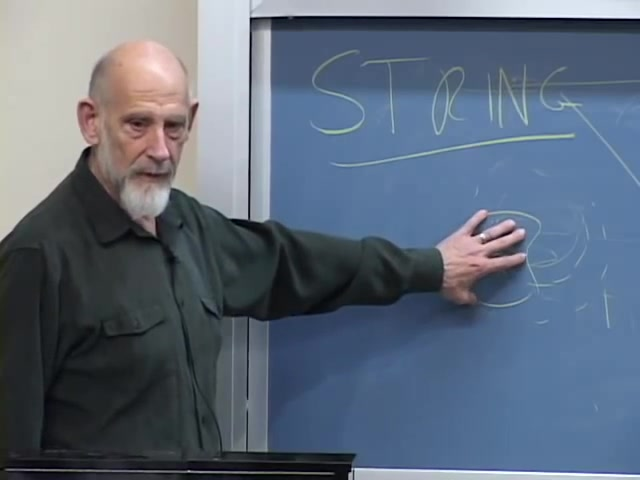
\includegraphics[width=0.60\textwidth]{lecture_09_figure_18.png}
\caption{讲座中的嵌套图景：严格受控的超对称弦构造位于一个推测上更大的框架之内。}
\lectureframe{01:57:34}
\end{figure}

\begin{classroomqa}
\audiencequestion{为什么不直接在精确理论中破缺超对称？\lecturetimestamp{01:57:02}}
\lecturerresponse{许多近似构造研究超对称破缺，但恰恰缺少的是完全可控的非超对称骨架。人们可以在作出标准近似之后进行计算，却并不总是知道这些近似所趋近的精确对象是什么。}
\end{classroomqa}

\begin{classroomqa}
\audiencequestion{精确的超对称理论是否排除了一个包含我们世界的更大、对称性更低的扩展？\lecturetimestamp{02:00:33}}
\lecturerresponse{不。它确立的是，观测到的世界并非仅由精确的超对称部分描述。它既未证明也未否证这一部分与一个包含现实物理的更大理论相关联。}
\end{classroomqa}

\begin{classroomqa}
\audiencequestion{弦构造是否包含类似于粒子物理对称性破缺的对称性破缺？\lecturetimestamp{02:01:21}}
\lecturerresponse{关于超对称破缺已有大量工作，对超对称数学也已有许多了解。尚未解决之处在于一个精确的非微扰表述，它将现实的破缺与完整理论结合起来，而不仅仅与可控近似结合起来。}
\end{classroomqa}

\begin{classroomqa}
\audiencequestion{狭义相对论在弦理论中是作为假设，还是作为预言而出现？\lecturetimestamp{02:03:02}}
\lecturerresponse{底层规则是洛伦兹不变的，尽管一个充满物质的特定背景可以选出一个优先的静止参考系。引力则更加不可避免：弦谱包含一个无质量自旋为二的激发态，其相互作用与引力子相同。}
\end{classroomqa}

\begin{classroomqa}
\audiencequestion{弦理论与广义相对论及背景无关性是否相容？\lecturetimestamp{02:04:11}}
\lecturerresponse{其低能引力动力学与广义相对论相容，并且局部背景可以被动力学地改变。微妙之处在于渐近边界条件：它们标记了问题本身，并且一般不能通过该时空内的局部操作来改变。}
\end{classroomqa}

讲座以稳健的数学核心与尚未完成的物理外推之间的这一区分作结。这并不是断言该核心无用，也不是声称该外推已经确立。它陈述的是精确知识止于何处。

\end{document}
